\documentclass[a4paper]{article}

\def\npart {III}
\def\nterm {Michaelmas}
\def\nyear {2017}
\def\nlecturer {C. Warnick}
\def\ncourse {Analysis of Partial Differential Equations}
\def\ncoursehead {Analysis of PDEs}

\usepackage{myheader}

\begin{document}
\maketitle
{\small
\setlength{\parindent}{0em}
\setlength{\parskip}{1em}

This course serves as an introduction to the mathematical study of Partial Differential Equations (PDEs). The theory of PDEs is nowadays a huge area of active research, and it goes back to the very birth of mathematical analysis in the 18th and 19th centuries. The subject lies at the crossroads of physics and many areas of pure and applied mathematics.

The course will mostly focus on four prototype linear equations: Laplace's equation, the heat equation, the wave equation and Schr\"odinger's equation. Emphasis will be given to modern functional analytic techniques, relying on a priori estimates, rather than explicit solutions, although the interaction with classical methods (such as the fundamental solution and Fourier representation) will be discussed. The following basic unifying concepts will be studied: well-posedness, energy estimates, elliptic regularity, characteristics, propagation of singularities, group velocity, and the maximum principle. Some non-linear equations may also be discussed. The course will end with a discussion of major open problems in PDEs.

\subsubsection*{Pre-requisites}
There are no specific pre-requisites beyond a standard undergraduate analysis background, in particular a familiarity with measure theory and integration. The course will be mostly self-contained and can be used as a first introductory course in PDEs for students wishing to continue with some specialised PDE Part III courses in the Lent and Easter terms.
}
\tableofcontents

\setcounter{section}{-1}
\section{Introduction}
Partial differential equations are ubiquitous in mathematics, physics, and beyond. The first equation we have met might be Laplace's equation, saying
\[
  -\Delta u = -\sum_{i = 1}^n \frac{\partial^2 u}{\partial x_i^2} = 0.
\]
This is the canonical example of an \emph{elliptic PDE}, and we will spend a lot of time thinking about elliptic PDEs, since they tend to be very well-behaved. Instead of trying to explicitly solve equations, as we did in, say, IB Methods, our focus is mostly on the existence and uniqueness of solutions, without explicitly constructing them. This will involve the use of machinery from functional analysis, and indeed a lot of the work will be about showing that we satisfy the hypotheses required by the functional-analytic results (as well as proving the functional-analytic results themselves (sometimes)).

We will also consider \emph{hyperbolic equations}. The canonical example is the wave equation
\[
  \frac{\partial^2 u}{\partial t^2} - \Delta u = 0.
\]
The difference is that the time derivative term now has a different sign from the rest. In Laplace's equation, all directions were equal. Here time is a ``special'' direction, and often our questions are about how the solution evolves in time.

Of course, we don't ``just solve'' such equations. Usually, we impose some \emph{data}, such as the desired values of $u$ on the boundary of our domain, or the ``starting configuration'' in the case of the wave equation. In general, given such a system, there are several questions we can ask:
\begin{itemize}
  \item Does a solution exist?
  \item Is the solution unique?
  \item Does the solution depend continuously on the data?
  \item How \emph{regular} is the solution? Is it continuously differentiable? Or even smooth?
\end{itemize}
These questions are closely related. To even make sense of the question, we need to specify our ``search space'', i.e.\ the sort of functions we are willing to consider. For example, we may consider the space of all smooth functions, or less ambitiously, the space of all twice-differentiable functions. This somewhat answers the last question, but it doesn't answer it completely. It could be that we can try to search for the solution in the space of $C^2$ functions, but it turns out the solutions are always smooth!

The choice of this function space affects the answers to the other questions as well. If we have a larger function space, then we are more likely to get a positive answer to the first question. However, since there are more functions around, we are more likely to get a \emph{negative} function to the second question. So there is some tension here.

The choice affects the third question in a slightly more subtle way. To speak of continuity, we must pick a topology, and this usually comes from a norm on the function space. Thus, to make sense of the third question, we must pick the appropriate norm on both the space of data and the space of potential solutions.

After choosing the appropriate function spaces, if the answers to the first three questions are all ``yes'', then we say the problem is \emph{well-posed}\index{well-posed problem}.

\section{Basics of PDEs}
It might be wise to define what a partial differential equation is.

\begin{defi}[Partial differential equation]
  Suppose $U \subseteq \R^n$ is open. A \term{partial differential equation} (\term{PDE}) of \emph{order}\index{order of PDE}\index{PDE!order} $k$ is a relation of the form
  \[
    F(x, u(x), \D u(x), \ldots, \D^k u(x)) = 0,\tag{$*$}
  \]
  where $F: U \times \R \times \R^n \times \R^{n^2} \times \cdots \times \R^{n^k} \to \R$ is a given function, and $u: U \to \R$ is the ``unknown''.
\end{defi}

\begin{defi}[Classical solution]
  We say $u \in C^k(U)$ is a \term{classical solution} of a PDE if in fact the PDE is identically satisfied on $U$ when $u, \D u, \ldots, \D^k u$ are substituted in.
\end{defi}

More generally, we can allow $u$ and $F$ to take values in a vector space. In this case, we say it is a \term{system of PDEs}\index{PDE!system}\index{partial differential equation!system}.

We can now entertain ourselves by writing out a large list of PDEs that are naturally found in physics and mathematics.
\begin{eg}[Transport equation]\index{transport equation}
  Suppose $v: \R^4 \times \R \to \R^3$ and $f: \R^4 \to \R$ are given. The \emph{transport equation} is
  \[
    \frac{\partial u}{\partial t}(x, t) + v(x, t, u(x, t)) \cdot \D_x u(x, t) = f(x, t)
  \]
  where we think of $x \in \R^3$ and $t \in \R$. This describes the evolution of the density $u$ of some chemical being advected by a flow $v$ and produced at a rate $f$.

  We see that this is a PDE of order $1$, and a relatively straightforward solution method exists, namely the \term{method of characteristics}.
\end{eg}

\begin{eg}[Laplace's and Poissson's equations]\index{Laplace's equation}\index{Poisson's equation}
  Taking $u: \R^n \to \R$, Laplace's equation is
  \[
    \Delta u(x) = \sum_{i = 1}^n \frac{\partial^2 u}{\partial x_i \partial x_i} (x) = 0.
  \]
  This describes, for example, the electrostatic potential in vacuum and the static distribution of heat inside a uniform solid body. It also has applications to steady flows in 2d fluids.

  There is an inhomogeneous version of this:
  \[
    \Delta u(x) = f(x),
  \]
  where $f: \R^n \to \R$ is a fixed function. This is known as \emph{Poisson's equation}, and describes, for example, the electrostatic field due to a charge distribution, and the gravitational field in Newtonian gravity.
\end{eg}

\begin{eg}[Heat/diffusion equation]\index{heat equation}\index{diffusion equation}
  This is given by
  \[
    \frac{\partial u}{\partial t} = \Delta u,
  \]
  where $u: \R^n \times \R \to \R$ is now a function of space and time. This describes the evolution of temperature inside a uniform body, or equivalently the diffusion of some chemical (where $u$ is the density).
\end{eg}

\begin{eg}[Wave equation]\index{wave equation}
  The wave equation is given by
  \[
    \frac{\partial^2 u}{\partial t^2} = \Delta u,
  \]
  where $u: \R^n \times \R \to \R$ is again a function of space and time. This describes oscillations of
  \begin{itemize}
    \item strings ($n = 1$)
    \item membrane/drum ($n = 2$)
    \item air density in a sound wave ($n = 3$)
  \end{itemize}
\end{eg}

\begin{eg}[Schr\"odinger's equation]\index{Schr\"odinger's equation}
  Let $u: \R^n \times \R \to \C \cong \R^2$. Up to choices of units and convention, the \emph{Schr\"odinger's equation} is
  \[
    i\frac{\partial u}{\partial t} + \Delta u - Vu = 0.
  \]
  Here $u$ is the wavefunction of a particle moving in a potential $V: \R^n \to \R$.
\end{eg}

\begin{eg}[Maxwell's equations]\index{Maxwell's equation}
  The unknowns here are $\mathbf{E}, \mathbf{B}: \R^3 \times \R \to \R^3$. They satisfy \emph{Maxwell's equations}
  \begin{align*}
    \nabla \cdot \mathbf{E} &= \rho & \nabla \cdot \mathbf{B} &= 0\\
    \nabla \times \mathbf{E} + \frac{\partial \mathbf{B}}{\partial t} &= 0 & \nabla \times \mathbf{B} - \frac{\partial \mathbf{E}}{\partial t} &= \mathbf{J},
  \end{align*}
  where $\rho$ is the electric charge density, $\mathbf{J}$ is the electric current, $\mathbf{E}$ is the electric field and $\mathbf{B}$ is the magnetic field.

  This is a system of 6 equations and 6 unknowns.
\end{eg}

\begin{eg}[Einstein's equations]\index{Einstein's equations}
  The \emph{Einstein's equation} in vacuum are
  \[
    R_{\mu\nu}[g] = 0,
  \]
  where $g$ is a Lorentzian metric (encoding the gravitational field), and $R_{\mu\nu}[g]$ is the Ricci curvature of $g$.

  Since we haven't said what $g$ and $R_{\mu\nu}$ are, it is not clear that this is a partial differential equation, but it is.
\end{eg}

\begin{eg}[Minimal surface equation]\index{minimal surface equation}
  The \emph{minimal surface equation is}
  \[
    \mathrm{Div}\left(\frac{\D u}{\sqrt{1 + |\D u|^2}}\right) = 0,
  \]
  where $u: \R^n \to \R$ is some function. This is the condition that the graph of $u$, $\{(x, u(x))\}\subseteq \R^n \times \R$, is locally an extremizer of area.
\end{eg}

\begin{eg}[Ricci flow]\index{Ricci flow}
  Let $g$ be a Riemannian metric on some manifold. The \emph{Ricci flow} is a PDE that evolves this metric:
  \[
    \frac{\partial g_{ij}}{\partial t} = R_{ij}[g],
  \]
  where $R_{ij}$ is again the Ricci curvature.

  The most famous application is in proving the Poincar\'e conjecture, which is a topological conjecture about $3$-manifolds.
\end{eg}

These PDEs exhibit a wide variety of behaviours. For example, waves behave very differently from the evolution of temperature. This means it is unlikely that we can say anything about PDEs as a whole, since everything we say must be true for both the heat equation and the wave equation. We must restrict to some particular classes of PDEs to say something useful. Thus, we seek to classify our PDEs into different types. We first introduce some notation.

%\subsubsection*{Data and well-posedness}
%In all the examples, we need some additional information to even hope for a unique solution. For example, in the case of Laplace's equation, we might need to know the boundary values of $u$; For the heat equation, we need to know the initial temperature distribution. We broadly refer to these information as the \term{data}. An important part of studying PDE is to understand what data we need for a certain PDE problem. Roughly speaking, we want enough data so that we can solve the problem, and not too much data that there is no solution.
%
%\begin{defi}[Well-posed problem]\index{well-posed problem}
%  We say a PDE problem (equation plus data) is \term{well-posed} if
%  \begin{enumerate}
%    \item A solution exists;
%    \item The solution is unique; and
%    \item The solution depends continuously on the data.
%  \end{enumerate}
%\end{defi}
%We should make this more precise. To say whether a solution exists, we need to first specify a function space, and ask if there is a solution in that function space. The same goes for the uniqueness problem. To ask whether the solution depends continuously, we must put the solution and data in appropriate function spaces that come with a topology.
%
%There is a certain freedom for us to choose which function space we are looking at, and there is no god-given choice. There is some tension between our requirements --- if we want our solution to exist, it is better to work with a larger function space; if we want it to be unique, we want it to be smaller. The details of whether a problem is well-posed can depend on the choice of function space.

In this course, the natural numbers start at $0$.
\begin{notation}[Multi-index/Schwartz notation]\index{multi-index notation}\index{Schwartz notation}
  We say an element $\alpha \in \N^n$ is a \emph{multi-index}. Writing $\alpha = (\alpha_1, \ldots, \alpha_n)$. We write
  \[
    |\alpha| = \alpha_1 + \alpha_2 + \cdots + \alpha_n.
  \]
  Also, we have
  \[
    \D^\alpha f = \frac{\partial^{|\alpha|}f}{\partial x_1^{\alpha_1} \partial x_2^{\alpha_2} \cdots \partial x_n^{\alpha_n}}.
  \]
  If $x = (x_1, \ldots, x_n) \in \R^n$, then
  \[
    x^\alpha = x_1^{\alpha_1} x_2^{\alpha_2} \cdots x_n^{\alpha_n}.
  \]
  We also write
  \[
    \alpha! = \alpha_1! \alpha_2! \cdots \alpha_n!.
  \]
\end{notation}

We now try to crudely classify the PDEs we have written down. Recall that our PDEs take the general form
\[
  F(x, u(x), \D u(x), \ldots, \D^k u(x)) = 0.
\]

\begin{defi}[Linear PDE]\index{linear PDE}\index{PDE!linear}
  We say a PDE is \emph{linear} if $F$ is a linear function of $u$ and its derivatives. In this case, we can re-write it as
  \[
    \sum_{|\alpha| \leq k} a_\alpha(x) \D^\alpha u = 0.
  \]
\end{defi}

\begin{defi}[Semi-linear PDE]\index{semi-linear PDE}\index{PDE!semi-linear}
  We say a PDE is \emph{semi-linear} if it is of the form
  \[
    \sum_{|\alpha| = k} a_\alpha(x) \D^\alpha u(x) + a_0[x, u, \D u, \ldots, \D^{k - 1} u] = 0.
  \]
  In other words, the terms involving the highest order derivatives are linear.
\end{defi}
Generalizing further, we have
\begin{defi}[Quasi-linear PDE]\index{quasi-linear PDE}\index{PDE!quasi-linear}
  We say a PDE is \emph{quasi-linear} if it is of the form
  \[
    \sum_{|\alpha| = k} a_\alpha [x, u, \D u, \ldots, \D^{k - 1} u] \D^\alpha u(x) + a_0[x, u, \ldots, \D^{k - 1} u] = 0.
  \]
\end{defi}
So the highest order derivative still appears linearly, but the coefficients can depend on lower-order derivatives of $u$.

Finally, we have
\begin{defi}[Fully non-linear PDE]\index{fully non-linear PDE}\index{PDE!fully non-linear}
  A PDE is \emph{fully non-linear} if it is not quasi-linear.
\end{defi}

\begin{eg}
  Laplace's equation $\Delta u = 0$ is linear.
\end{eg}

\begin{eg}
  The equation $u_{xx} + u_{yy} = u_x^2$ is semi-linear.
\end{eg}

\begin{eg}
  The equation $uu_{xx} + u_{yy} = u_x^2$ is quasi-linear.
\end{eg}

\begin{eg}
  The equation $u_{xx} u_{yy} - u_{xy}^2 = 0$ is fully non-linear.
\end{eg}

\section{The Cauchy--Kovalevskaya theorem}

\subsection{The Cauchy--Kovalevskaya theorem}
Before we begin talking about PDEs, let's recall what we already know about ODEs. Fix some $U \subseteq \R^n$ an open subset, and assume $f: U \to \R^n$ is given. Consider the ODE
\[
  \dot{u}(t) = f(u(t)).
\]
This is an \term{autonomous ODE}\index{ODE!autonomous} because there is no explicit $t$ dependence on the right. This assumption is usually harmless, as we can just increment $n$ and use the new variable to keep track of $t$. Here $u: (a, b) \to U$ is the unknown, where $a < 0 < b$.

The \term{Cauchy problem} for this equation is to find a solution to the ODE satisfying $u(0) = u_0 \in U$ for any $u_0$.

The Picard--Lindel\"of theorem says we can always do so under some mild conditions.
\begin{thm}[Picard--Lindel\"of theorem]\index{Picard--Lindelof theorem}
  Suppose that there exists $r, K > 0$ such that $B_r(u_0) \subseteq U$, and
  \[
    \|f(x) - f(y)\| \leq K \|x - u_0\|
  \]
  for all $x, y \in B_r(u_0)$. Then there exists an $\varepsilon > 0$ depending on $K, r$ and a unique $C^1$ function $u: (-\varepsilon, \varepsilon) \to U$ solving the Cauchy problem.
\end{thm}

It is instructive to give a quick proof sketch of the result.

\begin{proof}[Proof sketch]
  If $u$ is a solution, then by the fundamental theorem of calculus, we have
  \[
    u(t) = u_0 + \int_0^t f(u(s))\;\d s.
  \]
  Conversely, if $u$ is a $C^0$ solution to this integral equation, then it solves the ODE. Crucially, this only requires $u$ to be $C^0$. Indeed, if $u$ is $C^0$ and satisfies the integral equation, then $u$ is automatically $C^1$. So we can work in a larger function space when we seek for $u$.

  Thus, we have reformulated our initial problem into an integral equation. In particular, we reformulated it in a way that assumes less about the function. In the case of PDEs, this is what is known as a \term{weak formulation}.

  Returning to the proof, we have reformulated our problem as looking for a fixed point of the map
  \[
    B: w \mapsto u_0+ \int_0^t f(w(s))\;\d s
  \]
  acting on
  \[
    \mathcal{C} = \{w: [-\varepsilon, \varepsilon] \to \overline{B_{r/2}(u_0)} : w\text{ is continuous}\}.
  \]
  This is a complete metric space when we equip it with the supremum norm (in fact, it is a closed ball in a Banach space).

  We then show that for $\varepsilon$ small enough, this map $B: \mathcal{C} \to \mathcal{C}$ is a contraction map. There are two parts --- to show that it actually lands in $\mathcal{C}$, and that it is a contraction. If we managed to show these, then by the contraction mapping theorem, there is a unique fixed point, and we are done.
\end{proof}

The idea of formulating our problem as a fixed point problem is a powerful technique that allows us to understand many PDEs, especially non-linear ones. This theorem tells us that a unique $C^1$ solution exists locally. It is not reasonable to believe it can exist globally, as we might run out of $U$ in finite time. However, if $f$ is better behaved, we might expect $u$ to be more regular, and indeed this is the case. We shall not go into the details.

How can we actually use the theorem in practice? Can we actually obtain a solution from this? Recall that to prove the contraction mapping theorem, what we do is that we arbitrarily pick a point in $\mathcal{C}$, keep applying $\mathcal{B}$, and by the contraction, we must approach the fixed point. This gives us a way to construct an approximation to the ODE.

However, if we were a physicist, we would have done things differently. Suppose $f \in C^\infty$. We can then attempt to construct a Taylor series of the solution near the origin. First we note that for any solution $u$, we must have
\[
   u(0) = u_0,\quad \dot{u}(0) = f(u_0).
\]
Assuming $u$ is in fact a smooth solution, we can differentiate the ODE and obtain
\[
  \ddot{u}(t) = \frac{\d}{\d t} \dot{u}(t) = \frac{\d}{\d t} f(u(t)) = \D f(u(t)) \dot{u}(t) \equiv f_2(u(t), \dot{u}(t)).
\]
At the origin, we already know what $u$ and $\dot{u}$. We can proceed iteratively to determine
\[
  u^{(k)}(t) = f_k (u, \dot{u}, \ldots, u^{(k - 1)}).
\]
So in particular, we can in principle determine $u_k \equiv u^{(k)} = 0$. At least formally, we can write
\[
  u(t) = \sum_{k = 0}^\infty u_k \frac{t^k}{k!}.
\]
If we were physicists, we would say we are done. But being honest mathematicians, in order to claim that we have a genuine solution, we need to at least show that this converges. Under suitable circumstances, this is given by the Cauchy--Kovalevskaya theorem.

\begin{thm}[Cauchy--Kovalevskaya for ODEs]\index{Cauchy--Kovalevskaya theorem!for ODEs}\index{ODE!Cauchy--Kovalevskaya theorem}
  The series
  \[
    u(t) = \sum_{k = 0}^\infty u_k \frac{t^k}{k!}.
  \]
  converges to the Picard--Lindel\"of solution of the Cauchy problem if $f$ is real analytic in a neighbourhood of $u_0$.
\end{thm}

Recall that being real analytic means being equal to its Taylor series:
\begin{defi}[Real analytic]\index{real analytic}\index{analytic!real}
  Let $U \subseteq \R^n$ be open, and suppose $f: U \to \R$. We say $f$ is \emph{real analytic} near $x_0 \in U$ if there exists $r > 0$ and constants $f_\alpha \in \R$ for each multi-index $\alpha$ such that
  \[
    f(x) = \sum_\alpha f_\alpha (x - x_0)^\alpha
  \]
  for $|x - x_0| < r$.
\end{defi}

Note that if $f$ is real analytic near $x_0$, then it is in fact $C^\infty$ in the corresponding neighbourhood. Furthermore, the constants $f_\alpha$ are given by
\[
  f_\alpha = \frac{1}{\alpha!} \D^\alpha f(x_0).
\]
In other words, $f$ equals its Taylor expansion. Of course, by translation, we can usually assume $x_0 = 0$.

\begin{eg}
  If $r > 0$, set
  \[
    f(x) = \frac{r}{r - (x_1 + x_2 + \cdots + x_n)}
  \]
  for $|x| < \frac{r}{\sqrt{n}}$. Then this is real analytic, since we have
  \[
    f(x) = \frac{1}{1 - (x_1 + \cdots + x_n)/r} = \sum_{k = 0}^\infty \left(\frac{x_1 + \cdots + x_n}{r}\right)^k.
  \]
  We can then expand out each term to see that this is given by a power series. Explicitly, it is given by
  \[
    f(x) = \sum_\alpha \frac{1}{r^{|\alpha|}}\binom{|\alpha|}{\alpha} x^\alpha,
  \]
  where
  \[
    \binom{|\alpha|}{\alpha} = \frac{|\alpha|!}{\alpha!}.
  \]
  One sees that this series is absolutely convergent for $|x| < \frac{r}{\sqrt{n}}$.
\end{eg}
Recall that in single-variable analysis, essentially the only way we have to show that a series converges is by comparison to the geometric series. Here with multiple variables, our only way to show that a power series converges is by comparing it to this $f$.

\begin{defi}[Majorant]\index{majorant}\index{majorize}
  Let
  \[
    f = \sum_\alpha f_\alpha x^\alpha,\quad g = \sum_\alpha g_\alpha x^\alpha
  \]
  be formal power series. We say $g$ majorizes $f$ (or $g$ is a majorant of $f$), written $g \gg f$, if $g_\alpha \geq |f_\alpha|$ for all multi-indices $\alpha$.

  If $f$ and $A$ are vector-valued, then this means $g^i \gg f^i$ for all indices $i$.
\end{defi}

\begin{lemma}\leavevmode
  \begin{enumerate}
    \item If $g \gg f$ and $g$ converges for $|x| < r$, then $f$ converges for $|x| < r$.
    \item If $f(x) = \sum_\alpha f_\alpha x^\alpha$ converges for $x < r$ and $0 < s\sqrt{n} < r$, then $f$ has a majorant which converges on $|x| < s$. % check
  \end{enumerate}
\end{lemma}

\begin{proof}\leavevmode
  \begin{enumerate}
    \item Given $x$, define $\tilde{x} = (|x_1|, |x_2|, \ldots, |x_n|)$. We then note that
      \[
        \sum_\alpha |f_\alpha x^\alpha| = \sum_\alpha |f_\alpha| \tilde{x}^\alpha \leq \sum_\alpha g_\alpha \tilde{x}^\alpha = g(\tilde{x}).
      \]
      Since $|\tilde{x}| = |x| < r$, we know $g$ converges at $\tilde{x}$.
    \item Let $0 < s\sqrt{n} < r$ and set $y = s(1, 1, \ldots, 1)$. Then we have
      \[
        |y| = s \sqrt{n} < r.
      \]
      So by assumption, we know
      \[
        \sum_\alpha f_\alpha y^\alpha
      \]
      converges. A convergent series has bounded terms, so there exists $C$ such that
      \[
        |f_\alpha y^\alpha| \leq C
      \]
      for all $\alpha$. But $y^\alpha = s^{|\alpha|}$. So we know
      \[
        |f_\alpha| \leq \frac{C}{s^{|\alpha|}} \leq \frac{C}{s^{|\alpha|}} \frac{|\alpha|!}{\alpha!}.
      \]
      But then if we set
      \[
        g(x) = \frac{Cs}{s - (x_1 + \cdots + x_n)} = C \sum_\alpha \frac{|\alpha|!}{s^{|\alpha|}\alpha!} x^\alpha,
      \]
      we are done, since this converges for $|x| < \frac{s}{\sqrt{n}}$.\qedhere
  \end{enumerate}
\end{proof}

With this lemma in mind, we can now prove the Cauchy--Kovalevskaya theorem for first-order PDEs. This concerns a class of problems similar to the Cauchy problem for ODEs. We first set up our notation.

We shall consider functions $\mathbf{u}: \R^n \to \R^m$. Writing $\mathbf{x} = (x^1, \ldots, x^n) \in \R^n$, we will consider the last variable $x^n$ as being the ``time variable'', and the others as being space. However, for notational convenience, we will not write it as $t$. We will adopt the shorthand $x' = (x^1, \ldots, x^{n - 1})$, so that $\mathbf{x} = (x', x^n)$.

Suppose we are given two real analytic functions
\begin{align*}
  B: \R^m \times \R^{n - 1} &\to \Mat_{m \times m}(\R)\\
  \mathbf{c}: \R^m \times \R^{n - 1} &\to \R^m.
\end{align*}
We seek a solution to the PDE
\[
  \mathbf{u}_{x^n} = \sum_{j = 1}^{n - 1}B(\mathbf{u}, x') \mathbf{u}_{x_j} + \mathbf{c}(\mathbf{u}, x')
\]
subject to $\mathbf{u} = 0$ when $x^n = 0$. We shall not require a solution on all of $\R^n$, but only on an open neighbourhood of the origin. Consequently, we will allow for $B$ and $\mathbf{c}$ to not be everywhere defined, but merely convergent on some neighbourhood of the identity.

Note that we assumed $B$ and $\mathbf{c}$ do not depend on $x^n$, but this is not a restriction, since we can always introduce a new variable $u^{m + 1} = x^n$, and enlarge the target space.

\begin{thm}[Cauchy--Kovalevskaya theorem]\index{Cauchy--Kovalevskaya theorem!for PDEs}\index{PDE!Cauchy--Kovalevskaya theorem}
  Given the above assumptions, there exists a real analytic function $\mathbf{u} = \sum_\alpha \mathbf{u}_\alpha x^\alpha$ solving the PDE in a neighbourhood of the origin. Moreover, it is unique among real analytic functions.
\end{thm}

The uniqueness part of the proof is not difficult. If we write out $\mathbf{u}$, $B$ and $\mathbf{c}$ in power series and plug them into the PDE, we can then simply collect terms and come up with an expression for what $\mathbf{u}$ must be. This is the content of the following lemma:

\begin{lemma}
  For $k = 1, \ldots, m$ and $\alpha$ a multi-index in $\N^n$, there exists a polynomial $q_\alpha^k$ in the power series coefficients of $B$ and $\mathbf{c}$ such that any analytic solution to the PDE must be given by
  \[
    \mathbf{u} = \sum_{\alpha} \mathbf{q}_\alpha(B, \mathbf{c}) x^\alpha,
  \]
  where $\mathbf{q}_\alpha$ is the vector with entries $q_\alpha^k$.

  Moreover, all coefficients of $q_\alpha$ are non-negative.
\end{lemma}
Note that despite our notation, $\mathbf{q}$ is not a function of $B$ and $\mathbf{c}$ (which are themselves functions of $\mathbf{u}$ and $x$). It is a function of the coefficients in the power series expansion of $B$ and $\mathbf{c}$, which are some fixed constants.

This lemma proves uniqueness. To prove existence, we must show that this converges in a neighbourhood of the origin, and for this purpose, the fact that the coefficients of $q_\alpha$ are non-negative is crucial. After we have established this, we will use the comparison test to reduce the theorem to the case of a single, particular PDE, which we can solve by hand.

\begin{proof}
%  By assumption, we can expand $B$ and $\mathbf{c}$ as power series:
%  \begin{align*}
%    B_j(\mathbf{z}, x') &= \sum_{\gamma, \delta} B_{j, \gamma, \delta} z^\gamma x^\delta\\
%    \mathbf{c}(\mathbf{z}, x') &= \sum_{\gamma, \delta} \mathbf{c}_{\gamma, \delta} z^\gamma x^\delta
%  \end{align*}
%  and we can write the individual components as
%  \[
%    B_{j, \gamma, \delta} = (b^{k\ell}_{j, \gamma, \delta}),\quad \mathbf{c}_{\gamma, \delta} = (c^1_{\gamma, \delta}, \ldots, c^m_{\gamma, \delta}),
%  \]
%  for $j = 1, \ldots, n - 1$ and $k, \ell = 1, \ldots, m$.
%
%  Thus, in components, the PDE reads
%  \[
%    u^k_{x^n} = \sum_{j = 1}^{n - 1} \sum_{i = 1}^m b_j^{k\ell} (\mathbf{u}, x') u_{x_j}^\ell + c^k(\mathbf{u}, x')
%  \]
%  with the initial condition $u^k(x) = 0$.
  We construct the polynomials $q_\alpha^k$ by induction on $\alpha_n$. If $\alpha_n = 0$, then since $\mathbf{u} = 0$ on $\{x_n = 0\}$, we conclude that we must have
  \[
    u_\alpha = \frac{\D^\alpha \mathbf{u}(0)}{\alpha!} = 0.
  \]
  For $\alpha_n = 1$, we note that whenever $x^n = 0$, we have $\mathbf{u}_{x_j} = 0$ for $j = 1, \ldots, n - 1$. So the PDE reads
  \[
    \mathbf{u}_{x_n}(x', 0) = \mathbf{c}(0, x').
  \]
  Differentiating this relation in directions tangent to $x_n = 0$, we find that if $\alpha = (\alpha', 1)$, then
  \[
    \D^\alpha \mathbf{u}(0) = \D^{\alpha'} \mathbf{c}(0, 0).
  \]
  So $q_\alpha^k$ is a polynomial in the power series coefficients of $\mathbf{c}$, and has non-negative coefficients.

  Now suppose $\alpha_n = 2$, so that $\alpha = (\alpha', 2)$. Then
  \begin{align*}
    \D^\alpha \mathbf{u} &= \D^{\alpha'} (\mathbf{u}_{x^n})_{x^n}\\
    &= \D^{\alpha'} \left(\sum_j B_j \mathbf{u}_{x^j} + \mathbf{c}\right)_{x^n}\\
    &= \D^{\alpha'} \left(\sum_j \left(B_j \mathbf{u}_{x^j, x^n} + \sum_p \left(B_{u_p} \mathbf{u}_{x^j}\right) u^p_{x^n}\right) + \sum_p \mathbf{c}_{u_p} u^p_{x^n}\right)
  \end{align*}
  We don't really care what this looks like. The point is that when we evaluate at $0$, and expand all the terms out, we get a polynomial in the derivatives of $B_j$ and $\mathbf{c}$, and also $\D^\beta \mathbf{u}$ with $\beta_n < 2$. The derivatives of $B_j$ and $\mathbf{c}$ are just the coefficients of the power series expansion of $B_j$ and $\mathbf{c}$, and by the induction hypothesis, we can also express the $\D^\beta \mathbf{u}$ in terms of these power series coefficients. Thus, we can use this to construct $\mathbf{q}_\alpha$. By inspecting what the formula looks like, we see that all coefficients in $\mathbf{q}_\alpha$ are non-negative.

  We see that we can continue doing the same computations to obtain all $\mathbf{q}_\alpha$.
%
%  \begin{align*}
%    \D^\alpha u^k &= \D^{\alpha'}(u^k_{x_n})_{x_n}\\
%    &= \D^{\alpha'}\left(\sum_{j = 1}^{n - 1} \sum_{\ell = 1}^m b_j^{k\ell} u_{x_j}^\ell + c^k\right)_{x_n}\\
%    &= \D^{\alpha'}\left(\sum_{j = 1}^{n - 1} \sum_{\ell = 1}^m \left(b^{k\ell} u_{x_i x_n}^\ell + \sum_{p = 1}^m b^{k\ell}_{j, z_p} u^p_{x_n} u_{x_j}^{\ell}\right) + \sum_{p = 1}^m c_{z_p}^k u_{x_n}^p\right).
%  \end{align*}
%  Thus, we find that
%  \[
%     \D^{\alpha'} \left(\sum_{j = 1}^{n - 1} \sum_{\ell = 1}^m b_j^{k\ell} u_{x, x_n}^{\ell} + \sum_{p = 1}^m c_{z_p}^k u_{x_n}^p\right),
%  \]
%  evaluated at $0$.
%
%  We still have to expand out the right hand side. When we do so, it will be a polynomial with non-negative integer coefficients, involving derivatives of $B_j, \mathbf{c}$, and the derivatives $\D^\beta \mathbf{u}$, where $\beta_n \leq 1$. But we already know how to express $\D^\beta \mathbf{u}(0)$ in terms of the coefficients of $B$ and $\mathbf{c}$

%  In principle, we can keep on going, making the same (unpleasant) computations for each $\alpha$ and each $k = \{1, \ldots, m\}$. We find that $\D^\alpha u^k(0)$ is a polynomial in arbitrary derivatives of $B$ and $\mathbf{c}$, and derivatives $\D^\beta u^k$ with $\beta_n < \alpha_n$, and further the coefficients are non-neative integers.

%  Plugging it into the series expansion of $u$, and we can decide the same statement holds for $u^k_\alpha$ as well.
\end{proof}

%\begin{eg}
%  Consider the equations
%  \begin{align*}
%    u_y &= v_x - f\\
%    v_y &= - u_x,
%  \end{align*}
%  subject to the condition $u = v = 0$ on $y = 0$. This implies $u_x = v_x = 0$ on $y = 0$. In general,
%  \[
%      (\partial_x)^n u(x, 0) = (\partial_x)^n v(x, 0) = 0.
%  \]
%  In the other direction, we have
%  \[
%    u_y(x, 0) = - f(x, 0),\quad v_y(x, 0) = 0.
%  \]
%  So we find that
%  \begin{align*}
%    (\partial_x)^n \partial_y u(x, 0) &= -(\partial_x)^n y(x, 0)\\
%    (\partial_x)^n \partial_y v(x, 0) &= 0
%  \end{align*}
%  Going further, we find that
%  \begin{align*}
%    u_{yy} &= v_{xy} - f_y\\
%    v_{yy} &= u_{xy}
%  \end{align*}
%  and we can keep going on.
%\end{eg}

An immediate consequence of the non-negativity is that
\begin{lemma}
  If $\tilde{B}_j \gg B_j$ and $\tilde{\mathbf{c}} \gg \mathbf{c}$, then
  \[
    q_\alpha^k(\tilde{B}, \tilde{\mathbf{c}}) > q_\alpha^k(B, \mathbf{c}).
  \]
  for all $\alpha$. In particular, $\tilde{\mathbf{u}} \gg \mathbf{u}$.
\end{lemma}

%\begin{proof}[Proof continued]
%  What we have found is that if an analytic solution
%  \[
%    \mathbf{u} = \sum_{\alpha} \mathbf{u}_\alpha x^\alpha
%  \]
%  exists, then it must be given by
%  \[
%    u_\alpha^k = q_\alpha^k(\ldots, B_{j, \gamma, \delta}, \ldots, \mathbf{c}_{\gamma, \delta}, \ldots, \mathbf{u}_\beta, \ldots),
%  \]
%  where $q_\alpha^k$ is a \emph{universal} polynomial, i.e.\ it doesn't depend on $B, cb$ except through its arguments. Moreovver, $q_\alpha^k$ has \emph{non-negative} coefficients further, $\beta_n \leq \alpha_n - 1$ for any mlti-index on the RHS.
%
%  It remains to show that the series
%  \[
%    \mathbf{u} = \sum_\alpha \mathbf{u}_\alpha x^\alpha
%  \]
%  for the above choice of $\mathbf{u}_\alpha$ converges near $x = 0$. Let us first suppose that
%  \[
%    B_j^* \gg B_j,\quad \mathbf{c}^* \gg \mathbf{c},
%  \]
%  where
%  \begin{align*}
%    B_j^*(z, x) &= \sum_{\gamma, \delta} B^*_{j, \gamma, \delta} z^\gamma x^\delta,\\
%    c^*(z, x) &= \sum_{\gamma, \delta} c^*_{\gamma, \delta} z^\gamma x^\delta.
%  \end{align*}
%  We assume all these series converge for $|z| + |x'| < s$. This is possible by a previous lemma.
%
%  By definition, we have
%  \begin{align*}
%    |B_{j, \gamma, \delta}^{k\ell}| &\leq (B_{j, \gamma, \delta}^*)^{k\ell}\\
%    0 \leq |c_{\gamma, \delta}^k| \leq (C_{\gamma, \delta}^*)^k.
%  \end{align*}
%  We consider the modified problem
%  \[
%    \mathbf{u}^*_{x_n} = \sum_{j = 1}^{n - 1} B_j^*(\mathbf{u}^*, x') \mathbf{u}^*_{x_j} + \mathbf{c}^*(\mathbf{u}^*, x').
%  \]
%  on $|x'|^2 + x_n^2 < r$, and $\mathbf{u}^* = 0$ on $x_n = 0$. We might need to reduce $r$ so that $B_j^*$ and $\mathbf{c}^*$ converges, but that's okay.
%
%  Again, we seek a real analytic solution
%  \[
%    \mathbf{u}^* = \sum_\alpha \mathbf{u}_\alpha^* x^\alpha.
%  \]
%  We claim that $\mathbf{u}^* \gg \mathbf{u}$. We will then show that $\mathbf{u}^*$ converges, and hence we are done.
%
%  In other words, we want to show that
%  \[
%    0 \leq |u_\alpha^k| \leq (u_\alpha^*)^k. \tag{$\dagger$}
%  \]
%  We prove this by induction on $\alpha_n$. For $\alpha_n = 0$, we note htat
%  \[
%    u_\alpha^k = (u_\alpha^*)^k = 0.
%  \]
%  So this is good.
%
%  For the induction step, assume that $(\dagger)$ holds for $\alpha_n \leq a - 1$, and suppose $\alpha_n = a$. We then have
%  \begin{align*}
%    |u_\alpha^*| &= |q_\alpha^k(\ldots, B_{j, \gamma, \delta}^{k\ell}, \ldots, \mathbf{c}_{\gamma, \delta}^k, \ldots, \mathbf{u}_\beta^k)\\
%    &\leq q^k_\alpha (\ldots, |B_{j, \gamma, \delta}^{k\ell}|, \ldots, |\mathbf{c}_{\gamma, \delta}^k|, \ldots, |\mathbf{u}_\beta^k|)\\
%    &\leq q^k_\alpha (\ldots, (B_{j, \gamma, \delta}^*)^{k\ell}, \ldots, (\mathbf{c}_{\gamma, \delta}^*)^k, \ldots, (\mathbf{u}_\beta^*)^k)\\
%    &= (u^*_\alpha)^k,
%  \end{align*}
%  where we use the fact that $q_\alpha$ only has non-negative coefficients.
%
%  This gives $\mathbf{u}^* \gg \mathbf{u}$.
%
%  To show that $\mathbf{u}^*$ converges, we will make a particular choice for $B^*$ and $\mathbf{c}^*$, and solve the equation explicitly. Recall that when we proved the existence of majorizer, we actually wrote down an explicit choice of majorizors. They are given by
%\end{proof}

So given any $B$ and $\mathbf{c}$, if we can find some $\tilde{B}$ and $\tilde{\mathbf{c}}$ that majorizes $B$ and $\mathbf{c}$ respectively, and show that the corresponding series converges for $\tilde{B}$ and $\tilde{\mathbf{c}}$, then we are done.

But we previously saw that every power series is majorized by
\[
  \frac{Cr}{r - (x^1 + \cdots + x^n)}
\]
for $C$ sufficiently large and $r$ sufficiently small. So we have reduced the problem to the following case:
\begin{lemma}
  For any $C$ and $r$, define
  \[
    h(z, x') = \frac{Cr}{r - (x_1 + \cdots + x_{n - 1}) - (z_1 + \cdots + z_m)}
  \]
  If $B$ and $\mathbf{c}$ are given by
  \[
    B^*_j(z, x') = h(z, x') \begin{pmatrix}
      1 & \cdots & 1\\
      \vdots & \ddots & \vdots\\
      1 & \cdots & 1
    \end{pmatrix},\quad \mathbf{c}^*(z, x') = h(z, x')
    \begin{pmatrix}
      1 \\ \vdots \\ 1
    \end{pmatrix},
  \]
  then the power series
  \[
    \mathbf{u} = \sum_{\alpha} \mathbf{q}_\alpha(B, \mathbf{c}) x^\alpha
  \]
  converges in a neighbourhood of the origin.
\end{lemma}

We'll provide a rather cheap proof, by just writing down a solution of the corresponding PDE. The solution itself can be found via the method of characteristics, which we will learn about soon. However, the proof itself only requires the existence of the solution, not how we got it.
\begin{proof}
  We define
  \[
    v(x) = \frac{1}{mn} \left(r - (x^1 + \cdots + x^{n - 1}) - \sqrt{(r - (x^1 + \cdots + x^{n - 1}))^2 - 2mn Cr x^n}\right),
  \]
  which is real analytic around the origin, and vanishes when $x^n = 0$. We then observe that
  \[
    \mathbf{u}(x) = v(x)
    \begin{pmatrix}
      1\\\vdots\\1
    \end{pmatrix}
  \]
  gives a solution to the corresponding PDE, and is real analytic around the origin. Hence it must be given by that power series, and in particular, the power series must converge.
\end{proof}

%  which majorize $B_j$ and $\mathbf{c}$ provided $C$ is large enough and converge whenever $|x'| + |z| < s$ for some small $s$.
%
%  With these choices, the modified equation becomes
%  \[
%    (u_{x_n}^*)^k = \frac{C r}{ r - (x_1 + \cdots + x_n) - ((u^*)^1 + \cdots + (u^*)^n)} \left(\sum_{j = 1}^{k - 1} \sum_{\ell = 1}^m (u_{x_j}^*)^\ell + 1\right).
%  \]
%  It turns out this thing has an explicit solution
%  where
%  which we can check is real analytic near the origin.

\subsection{Reduction to first-order systems}

In nature, very few equations come in the form required by the Cauchy--Kovalevskaya theorem, but it turns out a lot of PDEs can be cast into this form after some work. We shall demonstrate this via an example.

\begin{eg}
  Consider the problem
  \begin{align*}
    u_{tt} &= uu_{xy} - u_{xx} + u_t\\
    u|_{t = 0} &= u_0\\
    u_t|_{t = 0} &= u_1,
  \end{align*}
  where $u_0, u_1$ are some real analytic functions near the origin. We define
  \[
    f = u_0 + t u_1.
  \]
  This is then real analytic near $0$, and $f|_{t = 0} = u_0$ and $f_t|_{t = 0} = u_1$. Set
  \[
    w = u - f.
  \]
  Then $w$ satisfies
  \[
    w_{tt} = ww_{xy} - w_{xx} + w_t + f w_{xy} + f_{xy}w + F,
  \]
  where
  \[
    F = ff_{xy} - f_{xx} + f_t,
  \]
  and
  \[
    w|_{t = 0} = w_t|_{t = 0} = 0.
  \]
  We let $(x, y, t) = (x^1, x^2, x^3)$ and set $\mathbf{u} = (w, w_x, w_y, w_t)$. Then our PDE becomes
  \begin{align*}
    u^1_t &= w_t = u^4\\
    u^2_t &= w_{xt} = u^4_x \\
    u^3_t &= w_{yt} = u^4_y\\
    u^4_t &= w_{tt} = u^1 u^2_{x_2} - u^2_{x_1} + u^4 + f u_{x_2}^2 + f_{xy}u^1 + F,
  \end{align*}
  and the initial condition is $\mathbf{u}(x^1, x^2, 0) = 0$. This is not quite autonomous, but we can solve that problem simply by introducing a further new variable.
\end{eg}

Let's try to understand this in more generality. In certain cases, it is not possible to write the equation in Cauchy--Kovalevskaya form. For example, if the equation has no local solutions, then it certainly cannot be written in that form, or else Cauchy--Kovalevskaya would give us a solution! It is thus helpful to understand when this is possible.

Note that in the formulation of Cauchy--Kovalevskaya, the derivative $\mathbf{u}_{x^n}$ is assumed to depend only on $x'$, and not $x^n$. If we want $\mathbf{u}_{x^n}$ to depend on $x^n$ as well, we can introduce a new variable $u^{n + 1}$ and set $(u^{n + 1})_{x^n} = 1$. So from now on, we shall ignore the fact that our PDE only has $x'$ on the right-hand side.

Let's now consider the scalar quasi-linear problem
\[
  \sum_{|\alpha| = k} a_\alpha(\D^{k - 1} u, \ldots, \D u, u, x) \D^\alpha u + a_0(\D^{k - 1}u, \ldots, u, x) = 0,
\]
where $u: B_r(0) \subseteq \R^n \to \R$, with initial data
\[
  u = \frac{\partial u}{\partial x_n} = \cdots = \frac{\partial^{k - 1} u}{\partial x_n^{k - 1}} = 0.
\]
whenever $|x'| < r$, $x_n = 0$.

We introduce a new vector
\[
  \mathbf{u} = \left(u, \frac{\partial u}{\partial x_1}, \ldots, \frac{\partial u}{\partial x_n}, \frac{\partial^2 u}{\partial x_1^2}, \ldots, \frac{\partial^{n - 1} u}{\partial x_n^{k - 1}}\right) = (u^1, \ldots, u^m)
\]
Here $\mathbf{u}$ contains all partial derivatives of $u$ up to order $k - 1$, for $j \in \{1, \ldots, m - 1\}$, we can compute $\frac{\partial u^j}{\partial x_n}$ in terms of $u^\ell$ or $\frac{\partial u^\ell}{\partial x^p}$ for some $\ell \in \{1, \ldots, m\}$ and $p < n$.

To express $\frac{\partial u^m}{\partial x_n}$ in terms of the other variables, we need to actually use the differential equation. To do so, we need to make an assumption about our equation. We suppose that $a_{(0, \ldots, 0, k)}(0, 0)$ is non-zero. We can then rewrite the equation as
\[
  \frac{\partial^k u}{\partial x_n^k} = \frac{-1}{a_{(0, \ldots, 0, k)}(\D^{k - 1}u, \ldots, u, x)} \left(\sum_{|\alpha| = k, \alpha_n < k} a_\alpha D^\alpha u + a_0\right),
\]
where at least near $x = 0$, the denominator can't vanish. The RHS can then be written in terms of $\frac{\partial u^k}{\partial x^p}$ and $ub$ for $p < n$.

So we have cast our original equation into the form we previously discussed, \emph{provided} that the $a_\alpha$'s and $a_0$'s are real analytic about the origin, and that $a_{(0, \ldots, 0, k)}(0, \ldots, 0) = 0$. Under these assumptions, we can solve the equation by Cauchy--Kovalevskaya.

It is convenient to make the following definition: if $a_{(0, \ldots, k)} (0, \ldots, 0) \not= 0$, we say $\{x_n = 0\}$ is \emph{non-characteristic}. Otherwise, we say it is \emph{characteristic}.

Often times, we want to specify our initial data on some more exotic surface. Unfortunately, they cannot be too exotic. They have to be real analytic in some sense for our theory to have any chance of working.

\begin{defi}[Real analytic hypersurface]\index{real analytic hypersurface}\index{hypersurface!real analytic}
  We say that $\Sigma \subseteq \R^n$ is a \emph{real analytic hypersurface} near $x \in \Sigma$ if there exists $\varepsilon > 0$ and a real analytic map $\Phi: B_\varepsilon(x) \to U \subseteq \R^n$, where $U = \Phi(B_\varepsilon(x))$, such that
  \begin{itemize}
    \item $\Phi$ is bijective and $\Phi^{-1}: U \to B_\varepsilon(x)$ is real analytic.
    \item $\Phi(\Sigma \cap B_\varepsilon(x)) = \{x_n = 0 \} \cap U$ and $\Phi(x) = 0$.
  \end{itemize}
\end{defi}
We think of this $\Phi$ as ``straightening out the boundary''.

Let $\gamma$ be the unit normal to $\Sigma$, and suppose $u$ solves
\[
  \sum_{|\alpha| = k} a_\alpha (\D^{k - 1} u, \ldots, u, x) \D^\alpha u + a_0(\D^{k - 1} u, \ldots, u, x) = 0
\]
subject to
\[
  u = \gamma^i \partial_i u = \cdots,(\gamma^i \partial_i)^{k- 1}u = 0
\]
on $\Sigma$.

To do so, we define $w(y) = u(\Phi^{-1}(y))$, so that
\[
  u(x) = w(\Phi(x)).
\]
Then by the chain rule, we have
\[
  \frac{\partial u}{\partial x_i} = \sum_{j = 1}^n \frac{\partial w}{\partial y_i} \frac{\partial \psi^j}{\partial x_i}.
\]
So plugging this into the equation, we see $w$ satisfies an equation of the form
\[
  \sum b_\alpha \D^\alpha w + b_0 = 0,
\]
as well as boundary conditions of
\[
  w = \frac{\partial w}{\partial y_n} = \cdots = \frac{\partial^{k - 1}w }{\partial y_n^{k - 1}} = 0.
\]
So we have transformed this to a quasi-linear equation with boundary conditions on $y_n = 0$, which we can tackle with Cauchy--Kovalevskaya, provided the surface $y_n = 0$ is non-characteristic. Can we relate this back to the $a$'s?

We can compute $b_{(0, \ldots, 0, k)}$ directly. Note that if $|\alpha| = k$, then
\[
  \D^\alpha u = \frac{\partial^k w}{\partial y_n^k} (\D \Phi^n)^\alpha + \text{terms not involving $\frac{\partial^n w}{\partial y_n^k}$}.
\]
So the coefficient of $\frac{\partial^k w}{\partial y_n^k}$ is
\[
  b_{(0, \ldots, k)} \sum_{|\alpha| = k} a_\alpha( \D \Phi^n)^\alpha.
\]
\begin{defi}[(Non-)characteristic surface]\index{non-characteristic surface}\index{characteristic surface}
  A surface $\Sigma$ is \emph{non-characteristic} at $x \Sigma$ provided
  \[
    \sum_{|\alpha| = k} a_\alpha (\D \Phi^n)^\alpha \not= 0.
  \]
  Equivalently, if
  \[
    \sum_{|\alpha| = k} a_\alpha \nu^\alpha \not= 0,
  \]
  where $\nu$ is the normal to the surface. We say a surface is \emph{characteristic} if it is not non-characteristic.
\end{defi}

We focus on the case where our PDE is second-order. Consider an operator of the form.
\[
  Lu = \sum_{i, j = 1}^n a_{ij} \frac{\partial^i u}{\partial x_i \partial x_j}
\]
where $a_{ij} \in \R$. We may wlog assume $a_{ij} = a_{ji}$. For example the wave equation and Laplace's equation are given by operators of this form. Consider the equation
\begin{align*}
  Lu &= f\\
  u = v^i \frac{\partial u}{\partial x^i} &= 0 \text{ on }\Pi_\nu = \{x \cdot \nu = 0\}.
\end{align*}
Then $\Pi_\nu$ is non-characteristic if
\[
  \sum_{i, j}^n a_{ij} \nu^i \nu^j \not= 0.
\]
Since $a_{ij}$ is diagonalizable, we see that if all eigenvalues are positive, then $\sum a_{ij} \nu^i \nu^j$ is non-zero, and so the problem has \emph{no} characteristic surfaces. In this case, we say the operator is \emph{elliptic}\index{elliptic operator}. If $(a_{ij})$ has one negative eigenvalue and the rest positive, then we say $L$ is \emph{hyperbolic}\index{hyperbolic operator}.

\begin{eg}
  If $L$ is the Laplacian
  \[
    L = \Delta = \sum_{i= 1}^n \frac{\partial^2}{\partial x_i^2},
  \]
  then $L$ is elliptic.

  If $L$ is the wave operator
  \[
    L = - \partial_t^2 + \Delta,
  \]
  then $L$ is hyperbolic.
\end{eg}

If we consider the problem
\[
  Lu = 0,
\]
and forget the Cauchy data, we can look for solutions of the form $e^{ik\cdot x}$, as a good physicist would do. We can plug this into our operator to compute
\[
  L(e^{ik\cdot x}) = - \sum_{i, j = 1}^n a_{ij} k^i k^j e^{ik\cdot x}.
\]
So if $L$ is elliptic, the only solution of this form is $k = 0$. If $L$ is hyperbolic, we can have non-trivial plane wave solutions provided $k \propto \nu$ for some $\nu$ with
\[
  \sum_{i, j = 1}^n a_{ij} \nu^i \nu^j = 0.
\]
So if we set $u_\lambda(x) = e^{i\lambda \nu \cdot x}$ for such a $\nu$ (with $|\nu| = 1$, wlog). By taking $\lambda$ very large, we can arrange this solution to have very large derivative in the $\nu$ direction. Vaguely, this says the characteristic directions are the directions where singularities can propagate. By contrast, we will see that this is not the case for elliptic operators, and this is known as \emph{elliptic regularity}. In fact, we will show that if $L$ is elliptic and $u$ satisfies $Lu = 0$, then $u \in C^\infty$.

While Cauchy--Kovalevskaya is sometimes useful, it has a few issues:
\begin{itemize}
  \item Not all functions are real analytic.
  \item We have no control over ``how long'' a solution exists.
  \item It doesn't answer the question of well-posedness.
\end{itemize}

Indeed, consider the PDE
\[
  u_{xx} + u_{yy} = 0.
\]
This admits a solution
\[
  u(x, y) = \cos kx \cosh ky
\]
for some $k \in \R$. We can think of this coming as coming from the Cauchy problem
\[
  u(x, 0) = \cos kx,\quad u_y(x, 0) = 0.
\]
By Cauchy--Kovalevskaya, there is a unique real analytic solution, and we've found one. So this is the unique solution.

Let's think about what happens when $k$ gets large. In this case, it seems like nothing is very wrong with the initial data. While the initial data oscillates more and more, it is still bounded by $1$. However, we see that the solution at any $y = \varepsilon > 0$ grows exponentially. We might say that the derivatives of the initial condition grows to infinity as well, but if we do a bit more work (as you will on the example sheet), we can construct a sequence of initial data all of whose derivatives tend to $0$, but the solution still blows up.

This is actually a serious problem. If we want to solve the PDE for a more general initial condition, we may want to decompose the initial data into Fourier modes, and then integrate up these solutions we found. But we cannot do this in general, if these solutions blow up as $k \to \infty$.

\section{Function spaces}
From now on, we shall restrain our desire to be a physicist, and instead tackle PDEs with functional analytic methods. This requires some technical understanding of certain function spaces.

\subsection{The \texorpdfstring{H\"older}{Holder} spaces}
The most straightforward class of functions paces is the $C^k$ spaces. These are spaces based on classical continuity and differentiability.

\begin{defi}[$C^k$ spaces]\index{$C^k(U)$}
  Let $U \subseteq \R^n$ be an open set. We define $C^k(U)$ to be vector space of all $u: U \to \R$ such that $u$ is $k$-times differentiable and the partial derivatives $\D^\alpha u : U \to \R$ are continuous for $|\alpha| \leq k$.
\end{defi}
We want to turn this into a Banach space by putting the supremum norm on the derivatives. However, even $\sup |u|$ is not guaranteed to exist, as $u$ may be unbounded. So this doesn't give a genuine norm. This suggests the following definition.

\begin{defi}[$C^k(\bar{U})$ spaces]\index{$C^k(\bar{U})$}
  We define $C^k(\bar{U}) \subseteq C^k(U)$ to be the subspace of all $u$ such that $\D^\alpha u$ are all bounded and uniformly continuous. We define a norm on $C^k(\bar{U})$ by
  \[
    \|u\|_{C^k(\bar{U})} = \sum_{|\alpha| \leq k} \sup_{x \in U} \|\D^\alpha u(x)\|.
  \]
  This makes $C^k(\bar{U})$ a Banach space.
\end{defi}

In some cases, we might want a ``fractional'' amount of differentiability. This gives rise to the notion of H\"older spaces.
\begin{defi}[H\"older continuity]\index{H\"older continuity}
  We say a function $u: U \to \R$ is \emph{H\"older continuous} with index $\gamma$ if there exists $C \geq 0$ such that
  \[
    |u(x) - u(y)| \leq C|x - y|^\gamma
  \]
  for all $x, y \in U$.

  We write $C^{0, \gamma}(\bar{U}) \subseteq C^0(\bar{U})$\index{$C^{0, \gamma}(\bar{U})$} for the subspace of all H\"older continuous functions with index $\gamma$.

  We define the $\gamma$-H\"older semi-norm by
  \[
    [u]_{C^{0, \gamma}(\bar{U})} = \sup_{x\not= y \in U} \frac{|u(x) - u(y)|}{|x - y|^\gamma}.
  \]
  We can then define a norm on $C^{0, \gamma}(\bar{U})$ by
  \[
    \|u\|_{C^{(0, \gamma}(\bar{U})} = \|u\|_{C^0(\bar{U})} + [u]_{C^{0, \gamma}(\bar{U})}.
  \]
  We say $u \in C^{k, \gamma}(\bar{U})$\index{$C^{k, \gamma}(\bar{U})$} if $u \in C^k(\bar{U})$ and $\D^\alpha u \in C^{0, \gamma}(\bar{U})$ for all $|\alpha| = k$, and we define
  \[
    \|u\|_{C^{k, \gamma}(\bar{U})} = \|u\|_{C^k(\bar{U})} + \sum_{|\alpha| = k} [\D^\alpha u]_{C^{0, \gamma}(\bar{U})}.
  \]
  This makes $C^{k, \gamma}(\bar{U})$ into a Banach space as well.
\end{defi}

Note that $C^{0, 1}(\bar{U})$ is the set of (uniformly) Lipschitz functions on $U$.

\subsection{Sobolev spaces}
The properties of H\"older spaces are not difficult to understand, but on the other hand they are not too useful. This is not too surprising, perhaps, because the supremum norm only sees the maximum of the function, and ignores the rest. In contrast, the $L^p$ norm takes into account the values at all points. This gives rise to the notion of Sobolev spaces.

\begin{defi}[$L^p$ space]\index{$L^p$ space}
  Let $U \subseteq \R^n$ be open, and suppose $1 \leq p \leq \infty$. We define the space \term{$L^p(U)$} by
  \[
    L^p(U) = \{u: U \to \R\text{ measurable} \mid \|u\|_{L^p(U)} < \infty\}/\{\text{equality a.e.}\}.
  \]
  where, if $p < \infty$, we define
  \[
    \|u\|_{L^p(U)} = \left(\int_U |u(x)|^p\;\d x\right)^{1/p},
  \]
  and
  \[
    \|u\|_{L^\infty(U)} = \inf \{C \geq 0 \mid |u(x)| \leq C\text{ almost everywhere}\}.
  \]
\end{defi}
\begin{thm}
  $L^P(U)$ is a Banach space with the $L^p$ norm.\fakeqed
\end{thm}
We can also define local versions of $L^p$ spaces by saying $u \in L^p_{loc}(U)$ if $u \in L^p(V)$ for every $V \Subset U$, i.e.\ $\bar{V} \subseteq U$ and $\bar{V}$ is compact. This is read as ``$V$ is \term{compactly contained} in $U$''. By working with $L^p_{loc}(U)$, we ignore any possible blowing up at the boundary. Note that $L^p_{loc}(U)$ is not Banach, but is a Fr\'echet space.

What we want to do is to define differentiability for these things. If we try to define them via limits, then we run into difficulties since the value of an element in $L^p(U)$ at a point is not well-defined. To proceed, we use the notion of a weak derivative.

\begin{defi}[Weak derivative]\index{weak derivative}
  Suppose $u, v \in L^1_{loc}(U)$ and $\alpha$ is a multi-index. We say that $v$ is the $\alpha$th weak derivative of $u$ if
  \[
    \int_U u \D^\alpha \phi \;\d x = (-1)^{|\alpha|} \int_U v \phi\;\d x
  \]
  for all $\phi \in C^\infty_c(U)$, i.e.\ for all smooth, compactly supported function on $U$. We write $v = \D^\alpha u$.
\end{defi}

Note that if $u$ is a genuine smooth function, then $\D^\alpha u$ is the $\alpha$th weak derivative of $u$, as integration by parts tells us.

For those who have seen distributions, this is the same as the definition of a distributional derivative, except here we require that the derivative is an $L^1_{loc}$ function.

\begin{lemma}
  Suppose $v, \tilde{v} \in L^1_{loc}(U)$ are both $\alpha$th weak derivatives of $u \in L^1_{loc}(U)$, then $v = \tilde{v}$ almost everywhere.
\end{lemma}

\begin{proof}
  For any $\phi \in C^\infty_c(U)$, we have
  \[
    \int_U (v - \tilde{v}) \phi \;\d x = (-1)^{|\alpha|}\int_U (u - u) \D^\alpha \phi\;\d x = 0.
  \]
  Therefore $v - \tilde{v} = 0$ almost everywhere.
\end{proof}

Now that we have weak derivatives, we can define the Sobolev spaces.

\begin{defi}[Sobolev space]\index{Sobolev space}
  We say that $u \in L^1_{loc}(U)$ belongs to the \emph{Sobolev space} \term{$W^{k, p}(U)$} if $u \in L^p(U)$ and $\D^\alpha u$ exists and is in $L^p(U)$ for all $|\alpha| \leq k$.

  If $p = 2$, we write $H^k(U) = W^{k, 2}(U)$\index{$H^k(U)$}, which will be a Hilbert space.

  If $p < \infty$, we define the $W^{k, p}(U)$ norm by
  \[
    \|u\|_{W^{k, p}(U)} = \left(\sum_{|\alpha| \leq k}\int_U |\D^\alpha u|^p \;\d x \right)^{1/p}.
  \]
  If $p = \infty$, we define
  \[
    \|u\|_{W^{k, \infty}(U)} = \sum_{|\alpha|\leq k} \|\D^\alpha u\|_{L^\infty(U)}.
  \]
  We denote by $W_0^{k, p}(U)$\index{$W_0^{k, p}(U)$} the completion of $C_c^\infty(U)$ in this norm (and again $H^k_0(U) = W^{k, 2}_0(U)$\index{$H^k_0(U)$}).
\end{defi}

To see that these things are somehow interesting, it would be nice to find some functions that belong to these spaces but not the $C^k$ spaces.

\begin{eg}
  Let $u = B_1(0)$ be the unit ball in $\R^n$, and set
  \[
    u(x) = |x|^{-\alpha}
  \]
  when $x \in U, x \not= 0$. Then for $x \not= 0$, we have
  \[
    \D_i u = \frac{-\alpha x_i}{|x|^{\alpha + 1}}.
  \]
  By considering $\phi \in C_c^\infty(B_1(0) \setminus \{0\})$, it is clear that if $u$ is weakly differentiable, then it must be given by
  \[
    D_i u = \frac{-\alpha x_i}{|a|^{\alpha + 1}}\tag{$*$}
  \]
  We can check that $u \in L^1_{loc} (U)$ iff $\alpha < n$, and $\frac{x_i}{|x|^{\alpha + 1}} \in L^1_{loc}(U)$ if $\alpha < n - 1$.

  So if we want $u \in W^{1, p}(U)$, then we must take $\alpha < n - 1$. To check $(*)$ is indeed the weak derivative, suppose $\phi \in C^\infty_c(U)$. Then integrating by parts, we get
  \[
    - \int_{U - B_\varepsilon(0)}u \phi_{x_i} \;\d x = \int_{U - B_\varepsilon(0)} \D_i u \phi \;\d x - \int_{\partial B_\varepsilon(0)} u \phi \nu^i \;\d S,
  \]
  where $\nu = (\nu^1, \ldots, \nu^n)$ is the inwards normal. We can estimate
  \[
    \left|\int_{\partial B_\varepsilon(0)}u \phi \nu^i \;\d S\right| \leq \|\phi\|_{L^\infty} \cdot \varepsilon^{-\alpha } \cdot C \varepsilon^{n - 1} \leq \tilde{C} \varepsilon^{n - 1 - \alpha} \to 0\text{ as }\varepsilon \to 0
  \]
  for some constants $C$ and $\tilde{C}$. So the second term vanishes. So by, say, dominated convergence, it follows that $(*)$ is indeed the weak derivative.

  Finally, note that $\D_i u \in L^p(U)$ iff $p(\alpha + 1) < n$. Thus, if $\alpha < \frac{n - p}{p}$, then $u \in W^{1, p}(U)$. Note that if $p > n$, then the condition becomes $\alpha < 0$, and $u$ is continuous.

  Note also that if $\alpha > \frac{n}{p}$, then $u \not \in W^{1,p}(U)$.
\end{eg}

\begin{thm}
  For each $k = 0, 1, \ldots$ and $1 \leq p \leq \infty$, the space $W^{k, p}(U)$ is a Banach space.
\end{thm}

\begin{proof}
  Homogeneity and positivity for the Sobolev norm are clear. The triangle inequality follows from the Minkowski inequality.

  For completeness, note that
  \[
    \|\D^\alpha u\|_{L^p(U)} \leq \|u\|_{W^{k, p}(U)}
  \]
  for $|\alpha| \leq k$.

  So if $(u_i)_{i = 1}^\infty$ is Cauchy in $W^{k, p}(U)$, then $(\D^\alpha u_i)_{i = 1}^\infty$ is Cauchy in $L^p(U)$ for $|\alpha| \leq k$. So by completeness of $L^p(U)$, we have
  \[
    \D^{\alpha}u_i \to u^\alpha \in L^p(U)
  \]
  for some $u^\alpha$. It remains to show that $u^\alpha = \D^\alpha u$, where $u = u^{(0, 0, \ldots, 0)}$. Let $\phi \in C_c^\infty(U)$. Then we have
  \[
    (-1)^{|\alpha|} \int_U u_j \D^\alpha \phi \;\d x = \int_U \D^\alpha u_j \phi\;\d x
  \]
  for all $j$. We send $j \to \infty$. Then using $\D^\alpha u_j \to u^\alpha$ in $L^p(U)$, we have
  \[
    (-1)^{|\alpha|} \int_U u \D^\alpha \phi\;\d x = \int_U u^\alpha \phi\;\d x.
  \]
  So $\D^\alpha u = u^\alpha \in L^p(U)$ and we are done.
\end{proof}

\subsection{Approximation of functions in Sobolev spaces}
It would be nice if we could approximate functions in $W^{k, p}(U)$ with something more tractable. For example, it would be nice if we could approximate them by smooth functions, so that the weak derivatives are genuine derivatives. A useful trick to improve regularity of a function is to convolve with a smooth mollifier.

\begin{defi}[Standard mollifier]\index{standard mollifier}\index{mollifier!standard}
  Let
  \[
    \eta(x) =
    \begin{cases}
      C e^{1/(|x|^2 - 1)}& |x| < 1\\
      0 & |x| \geq 1
    \end{cases} ,
  \]
  where $C$ is chosen so that $\int_{\R^n} \eta(x) \;\d x = 1$.
  \begin{center}
    \begin{tikzpicture}[xscale=1.5]
      \draw (-2, 0) -- (2, 0);
      \draw [->] (0, 0) -- (0, 2.5);
      \draw [domain=-0.99:0.99, thick, mblue, samples=50] plot (\x, {5 * exp(1/((\x)^2 - 1))});
      \draw [thick, mblue] (-2, 0) -- (-0.99, 0);
      \draw [thick, mblue] (2, 0) -- (0.99, 0);
    \end{tikzpicture}
  \end{center}
  One checks that this is a smooth function on $\R^n$, peaked at $x = 0$.

  For each $\varepsilon > 0$, we set
  \[
    \eta_\varepsilon(x) = \frac{1}{\varepsilon^n} \eta\left(\frac{x}{\varepsilon}\right).
  \]
  Of course, the pre-factor of $\frac{1}{\varepsilon^n}$ is chosen so that $\eta_\varepsilon$ is appropriately normalized.

  We call $\eta_\varepsilon$ the \emph{standard mollifier}, and it satisfies $\supp \eta_\varepsilon \subseteq \overline{B_\varepsilon(0)}$.
\end{defi}
We think of these $\eta_\varepsilon$ as approximations of the $\delta$-function.

Now suppose $U \subseteq \R^n$ is open, and let
\[
  U_\varepsilon = \{x \in U: \mathrm{dist}(x, \partial U) > \varepsilon\}.
\]
\begin{defi}[Mollification]\index{mollification}
  If $f \in L^1_{loc}(U)$, we define the \term{mollification} $f_\varepsilon: U_\varepsilon \to \R$ by the convolution
  \[
    f_\varepsilon = \eta_\varepsilon * f.
  \]
  In other words,
  \[
    f_\varepsilon(x) = \int_U \eta_\varepsilon (x - y) f(y) = \int_{B_\varepsilon(x)} \eta_\varepsilon(x - y) f(y)\;\d y.
  \]
\end{defi}
Thus, $f_\varepsilon$ is the ``local average'' of $f$ around each point, with the weighting given by $\eta_\varepsilon$. The hope is that $f_\varepsilon$ will have much better regularity properties than $f$.

\begin{thm}
  Let $f \in L^1_{loc}(U)$. Then
  \begin{enumerate}
    \item $f_\varepsilon \in C^\infty(U_\varepsilon)$.
    \item $f_\varepsilon \to f$ almost everywhere as $\varepsilon \to 0$.
    \item If in fact $f \in C(U)$, then $f_\varepsilon \to f$ uniformly on compact subsets.
    \item If $1 \leq p < \infty$ and $f \in L^p_{loc}(U)$, then $f_\varepsilon \to f$ in $L^p_{loc}(U)$, i.e.\ we have convergence in $L^p$ on any $V \Subset U$.\fakeqed
  \end{enumerate}
\end{thm}
In general, the difficulty of proving these approximation theorems lie in what happens at the boundary
\begin{lemma}
  Assume $u \in W^{k, p}(U)$ for some $1 \leq p < \infty$, and set
  \[
    u_\varepsilon = \eta_\varepsilon * u\text{ on }U_\varepsilon.
  \]
  Then
  \begin{enumerate}
    \item $u_\varepsilon \in C^\infty(U_\varepsilon)$ for each $\varepsilon > 0$
    \item If $V \Subset U$, then $u_\varepsilon \to u$ in $W^{k, p}(V)$.
  \end{enumerate}
\end{lemma}

\begin{proof}\leavevmode
  \begin{enumerate}
    \item As above.
    \item We claim that
      \[
        \D^\alpha u_\varepsilon = \eta_\varepsilon * D^\alpha u
      \]
      for $|\alpha| \leq k$ in $U_\varepsilon$.

      To see this, we have
      \begin{align*}
        \D^\alpha u^\varepsilon(x) &= \D^\alpha \int_U \eta_\varepsilon(x - y) u(y) \;\d y\\
        &= \int_U \D^\alpha_x \eta_\varepsilon (x - y) u(y)\;\d y\\
        &= \int_U (-1)^{|\alpha|} \D_y^\alpha \eta_\varepsilon(x - y) u(y)\;\d y\\
        \intertext{For a fixed $x \in U_\varepsilon$, $\eta_\varepsilon(x - \ph) \in C_c^\infty(U)$, so by the definition of a weak derivative, this is equal to}
        &= \int_U \eta_\varepsilon(x - y) \D^\alpha u(y)\;\d y\\
        &= \eta_\varepsilon * \D^\alpha u.
      \end{align*}
      It is an exercise to verify that we can indeed move the derivative past the integral.

      Thus, if we fix $V \Subset U$. Then by the previous parts, we see that $\D^\alpha u_\varepsilon \to \D^\alpha u$ in $L^p(V)$ as $\varepsilon \to 0$ for $|\alpha| \leq k$. So
      \[
        \|u_\varepsilon - u\|^p_{W^{k. p}(V)} = \sum_{|\alpha| \leq k} \|\D^\alpha u_\varepsilon - \D^\alpha u\|^p_{L^p(V)} \to 0
      \]
      as $\varepsilon \to 0$.\qedhere
  \end{enumerate}
\end{proof}

\begin{thm}[Global approximation]\index{global approximation}
  Let $1 \leq p < \infty$, and $U \subseteq \R^n$ be open and bounded. Then $C^\infty(U) \cap W^{k, p}(U)$ is dense in $W^{k, p}(U)$.
%
%  $u \in W^{k. p}(U)$ with $1 \leq p < \infty$. Then
%
%  Then there exists $u_m \in C^\infty(U) \cap W^{k, p}(U)$ such that $u_m \to u$ in $W^{k, p}(U)$.
%
%  In other words, $C^\infty(U) \cap W^{k. p}(U)$ is dense in $W^{k, p}(U)$.
\end{thm}
Our main obstacle to overcome is the fact that the mollifications are only defined on $U_\varepsilon$, and not $U$.

\begin{proof}
  For $i \geq 1$, define
  \begin{align*}
    U_i &= \left\{x \in U \mid \mathrm{dist}(x, \partial U) > \tfrac{1}{i}\right\}\\
    V_i &= U_{i + 3} - \bar{U}_{i + 1}\\
    W_i &= U_{i + 4} - \bar{U}_i.
  \end{align*}
  We clearly have $U = \bigcup_{i = 1}^\infty U_i$, and we can choose $V_0 \Subset U$ such that $U = \bigcup_{i = 0}^\infty V_i$.

  Let $\{\zeta_i\}_{i = 0}^\infty$ be a partition of unity subordinate to $\{V_i\}$. Thus, we have $0 \leq \zeta_i \leq 1$, $\zeta_i \in C_c^\infty(V_i)$ and $\sum_{i = 0}^\infty \zeta_i = 1$ on $U$.

  Fix $\delta > 0$. Then for each $i$, we can choose $\varepsilon_i$ sufficiently small such that
  \[
    u^i = \eta_{\varepsilon_i} * \zeta_i u
  \]
  satisfies $\supp u_i \subseteq W_i$ and
  \[
    \|u_i - \zeta_i u\|_{W^{k. p}(U)} = \|u_i - \zeta_i u\|_{W^{k. p}(W_i)} \leq \frac{\delta}{2^{i + 1}}.
  \]
  Now set
  \[
    v = \sum_{i = 0}^\infty u_i \in C^\infty(U).
  \]
  Note that we do not know (yet) that $v \in W^{k. p}(U)$. But it certainly is when we restrict to some $V \Subset U$.

  In any such subset, the sum is finite, and since $u = \sum_{i = 0}^\infty \zeta_i u$, we have
  \[
    \|v - u\|_{W^{k, p}(V)} \leq \sum_{i = 0}^\infty \|u^i - \zeta_i u\|_{W^{k. p}(V)} \leq \delta \sum_{i = 0}^\infty 2^{-(i + 1)} = \delta.
  \]
  Since the bound $\delta$ does not depend on $V$, by taking the supremum over all $V$, we have
  \[
    \|v - u\|_{W^{k. p}(U)} \leq \delta.
  \]
  So we are done.
\end{proof}

It would be nice for $C^\infty(\bar{U})$ to be dense, instead of just $C^\infty(U)$. It turns out this is possible, as long as we have a sensible boundary.

\begin{defi}[$C^{k, \delta}$ boundary]\index{$C^{k, \delta}$ boundary}
  Let $U \subseteq \R^n$ be open and bounded. We say $\partial U$ is $C^{k, \delta}$ if for any point in the boundary $p \in \partial U$, there exists $r > 0$ and a function $\gamma \in C^{k, \delta}(\R^{n - 1})$ such that (possibly after relabelling and rotating axes) we have
  \[
    U \cap B_r(p) = \{(x', x_n) \in B_r(p): x_n > \gamma(x')\}.
  \]
\end{defi}
Thus, this says our boundary is locally the graph of a $C^{k, \delta}$ function.

\begin{thm}[Smooth approximation up to boundary]
  Let $1 \leq p < \infty$, and $U \subseteq \R^n$ be open and bounded. Suppose $\partial U$ is $C^{0, 1}$. Then $C^\infty(\bar{U}) \cap W^{k, p}(U)$ is dense in $W^{k, p}(U)$.
\end{thm}

\begin{proof}
  Previously, the reason we didn't get something in $C^\infty(\bar{U})$ was that we had to glue together infinitely many mollifications whose domain collectively exhaust $U$, and there is no hope that the resulting function is in $C^\infty(\bar{U})$. In the current scenario, we know that $U$ locally looks like
  \begin{center}
    \begin{tikzpicture}
      \fill [gray, opacity=0.3] (0, 0) .. controls (1, -0.3) and (1.5, 0.1) .. (2, 0.2) .. controls (2.5, 0.3) .. (3.4, 0) -- (3.4, 1) -- (0, 1) -- cycle;
      \draw (0, 0) .. controls (1, -0.3) and (1.5, 0.1) .. (2, 0.2) .. controls (2.5, 0.3) .. (3.4, 0);

      \node [circ] at (2, 0.2) {};
      \node [below] at (2, 0.2) {\small$x_0$};
    \end{tikzpicture}
  \end{center}
  The idea is that given a $u$ defined on $U$, we can shift it downwards by some $\varepsilon$. It is a known result that translation is continuous, so this only changes $u$ by a tiny bit. We can then mollify with a $\bar{\varepsilon} < \varepsilon$, which would then give a function defined on $U$ (at least locally near $x_0$).

  So fix some $x_0 \in \partial U$. Since $\partial U$ is $C^{0, 1}$, there exists $r > 0$ such that $\gamma \in C^{0, 1}(\R^{n - 1})$ such that
  \[
    U \cap B_r(x_0) = \{(x', x_n) \in B_r(x') \mid x_n > \gamma(x')\}.
  \]
  Set
  \[
    V = U \cap B_{r/2}(x^0).
  \]
  Define the shifted function $u_\varepsilon$ to be
  \[
    u_\varepsilon(x) = u(x + \varepsilon e_n).
  \]
  Now pick $\bar{\varepsilon}$ sufficiently small such that
  \[
    v^{\varepsilon, \bar{\varepsilon}} = \eta_{\bar{\varepsilon}} * u_\varepsilon
  \]
  is well-defined. Note that here we need to use the fact that $\partial U$ is $C^{0, 1}$. Indeed, we can see that if the slope of $\partial U$ is very steep near a point $x$:
  \begin{center}
    \begin{tikzpicture}
      \fill [gray, opacity=0.3] (0, 0) -- (0.5, 1.5) -- (0.5, 1.7) -- (0, 1.7);
      \draw (0, 0) -- (0.5, 1.5);

      \draw [dashed] (0, -0.3) -- (0.5, 1.2);

      \draw [-latex'] (0.6, 1.2) -- (0.6, 1.5) node [pos=0.5, right] {\small$\varepsilon$};
      \draw [latex'-] (0.6, 1.2) -- (0.6, 1.5);
    \end{tikzpicture}
  \end{center}
  then we need to choose a $\bar{\varepsilon}$ much smaller than $\varepsilon$. By requiring that $\gamma$ is $1$-H\"older continuous, we can ensure there is a single choice of $\bar{\varepsilon}$ that works throughout $V$. As long as $\bar{\varepsilon}$ is small enough, we know that $v^{\varepsilon, \bar{\varepsilon}} \in C^\infty(\bar{V})$.

  Fix $\delta > 0$. We can now estimate
  \begin{align*}
    \|v^{\varepsilon, \tilde{\varepsilon}} - u\|_{W^{k. p}(V)} &= \|v^{\varepsilon, \tilde{\varepsilon}} - u_\varepsilon + u_\varepsilon - u\|_{W^{k, p}(V)}\\
    &\leq \|v^{\varepsilon, \tilde{\varepsilon}} - u_\varepsilon\|_{W^{k, p}(V)} + \|u_\varepsilon - u\|_{W^{k. p}(V)}.
  \end{align*}
  Since translation is continuous in the $L^p$ norm for $p < \infty$, we can pick $\varepsilon > 0$ such that $\|u_\varepsilon - u\|_{W^{k. p}(V)} < \frac{\delta}{2}$. Having fixed such an $\varepsilon$, we can pick $\tilde{\varepsilon}$ so small that we also have $\|v^{\varepsilon, \tilde{\varepsilon}} - u_\varepsilon\|_{W^{k. p}(V)} < \frac{\delta}{2}$.

  The conclusion of this is that for any $x_0 \in \partial U$, we can find a neighbourhood $V \subseteq U$ of $x_0$ in $U$ such that for any $u \in W^{k, p}(U)$ and $\delta > 0$, there exists $v \in C^\infty(\bar{V})$ such that $\|u - v\|_{W^{k, p}(V)} \leq \delta$.

  It remains to patch all of these together using a partition of unity. By the compactness of $\partial U$, we can cover $\partial U$ by finitely many of these $V$, say $V_1, \ldots, V_N$. We further pick a $V_0$ such that $V_0 \Subset U$ and
  \[
    U = \bigcup_{i = 0}^N V_i.
  \]
  We can pick approximations $v_i \in C^\infty(\bar{V}_i)$ for $i = 0, \ldots, N$ (the $i = 0$ case is given by the previous global approximation theorem), satisfying $\|v_i - u\|_{W^{k, p}(V_i)} \leq \delta$.
%
%  Define the shifted point
%  \[
%    x^{\varepsilon} = x + \lambda\varepsilon e_n
%  \]
%  for $x \in V$, $\varepsilon > 0$.
%
%  For $\lambda > 0$ large enough and $\varepsilon$ sufficiently small, we have
%  \[
%    B_\varepsilon(x') \subseteq U \cap B_r(x^0).
%  \]
%  We can do this uniformly for all points $x \in V$ by the fact that $\gamma \in C^{0, 1}$.
%
%  We define $u_\varepsilon(x) = u(x^\varepsilon)$ for all $x \in V$. Set
%  \[
%    v^{\varepsilon, \tilde{\varepsilon}} = \eta_{\tilde{\varepsilon}} * u_\varepsilon
%  \]
%  for some $0 < \tilde{\varepsilon} < \varepsilon$. As a result, $v^{\varepsilon, \tilde{\varepsilon}} \in C^\infty(\bar{V})$.
%
%  Now fix $\delta > 0$. We estimate
%  \begin{align*}
%    \|v^{\varepsilon, \tilde{\varepsilon}} - u\|_{W^{k. p}}(V) &= \|v^{\varepsilon, \tilde{\varepsilon}} - u_\varepsilon + u_\varepsilon - u\|_{W^{k, p}(V)}\\
%    &\leq \|v^{\varepsilon, \tilde{\varepsilon}} - u_\varepsilon\|_{W^{k, p}(V)} + \|u_\varepsilon - u\|_{W^{k. p}(V)}.
%  \end{align*}
%  Since translation is continuous in the $L^p$-norms for $p < \infty$, we can pick $\varepsilon > 0$ such that $\|u_\varepsilon - u\|_{W^{k p}(V)} < \frac{\delta}{2}$.
%
%  Having fixed $\varepsilon$, we can then pick $\tilde{\varepsilon}$ so that $\|v^{\varepsilon, \tilde{\varepsilon}} - u_\varepsilon\|_{W^{k. p}(V)} < \frac{\delta}{\varepsilon}$.
%
%  Now since $\partial U$ is compact, we can cover $\partial U$ by finitely many of these $V$'s. More precisely, we can find finitely many $x_i^0 \in \partial U$, radii $r_i > 0$, sets $V_i = U \cap B_{r_i/2}(x_i^0)$ and functions $v_i \in C^\infty(\bar{V}_i)$ for $i = 1, \ldots, N$, such that
%  \[
%    \partial U \subseteq \bigcup_{i = 1}^N B_{r_i/2}(x_i^0).
%  \]
%  and
%  \[
%    \|v_i - u\|_{W^{k, p}(V_i)} \leq \delta.
%  \]
%  Finally, take an open $V_0 \Subset U$ such that
%  \[
%    C \subseteq \cup_{i = 0}^N V_i.
%  \]
%  By the previous theorem, we can choose $v_0 \in C^{\infty}(\bar{V}_0$ such that $\|v_0 - u\|_{W^{k, p}(V_0)} \leq \delta$.
%
  Pick a partition of unity $\{\zeta_i\}_{i = 0}^N$ of $\bar{U}$ subordinate to $\{V_i\}$. Define
  \[
    v = \sum_{i = 0}^N \zeta_i v_i.
  \]
  Clearly $v \in C^\infty(\bar{U})$, and we can bound
  \begin{align*}
    \|D^\alpha v - \D^\alpha u\|_{L^p(U)} &= \norm{\D^\alpha \sum_{i = 0}^N \zeta_i v_i - \D^\alpha \sum_{i = 0}^N \zeta_i u}_{L^p(U)}\\
    &\leq C_k \sum_{i = 0}^N \|v_i - u\|_{W^{k. p}(V_i)}\\
    &\leq C_k(1 + N)\delta,
  \end{align*}
  where $C_k$ is a constant that solely depends on the derivatives of the partition of unity, which are fixed. So we are done.
\end{proof}

\subsection{Extensions and traces}
If $U \subseteq \R^n$ is open and bounded, then there is of course a restriction map $W^{1, p}(\R^n) \to W^{1, p}(U)$. It turns out under mild conditions, there is an extension map going in the other direction as well.

\begin{thm}[Extension of $W^{1. p}$ functions]
  Suppose $U$ is open, bounded and $\partial U$ is $C^1$. Pick a bounded $V$ such that $U \Subset V$. Then there exists a bounded linear operator
  \[
    E: W^{1, p}(U) \to W^{1. p}(\R^n)
  \]
  for $1 \leq p < \infty$ such that for any $u \in W^{1, p}(U)$,
  \begin{enumerate}
    \item $Eu = u$ almost everywhere in $U$
    \item $Eu$ has support in $V$
    \item $\|Eu\|_{W^{1, p}(\R^n)} \leq C \|u\|_{W^{1, p}(U)}$, where the constant $C$ depends on $U, V, p$ but not $u$.
  \end{enumerate}
\end{thm}

\begin{proof}
  First note that $C^1(\bar{U})$ is dense in $W^{1, p}(U)$. So it suffices to show that the above theorem holds with $W^{1, p}(U)$ replaced with $C^1(\bar{U})$, and then extend by continuity.

  We first show that we can do this locally, and then glue them together using partitions of unity.

  Suppose $x^0 \in \partial U$ is such that $\partial U$ near $x^0$ lies in the plane $\{x_n = 0\}$. In other words, there exists $r > 0$ such that
  \begin{align*}
    B_+ &= B_r(x^0) \cap \{x_n \geq 0\} \subseteq \bar{U}\\
    B_- &= B_r(x^0) \cap \{x_n \leq 0\} \subseteq \R^n \setminus U.
  \end{align*}
  The idea is that we want to reflect $u|_{B_+}$ across the $x_n = 0$ boundary to get a function on $B_{-}$, but the derivative will not be continuous if we do this. So we define a ``higher order reflection'' by
  \[
    \bar{u}(x) =
    \begin{cases}
      u(x) & x \in B^+\\
      -3u(x', -x_n) + 4\left(u x', -\frac{x_n}{2}\right) & x \in B_-
    \end{cases}
  \]
  \begin{center}
    \begin{tikzpicture}
      \draw [->] (-3, 0) -- (3, 0) node [right] {$x^n$};
      \draw [->] (0, -3) -- (0, 3) node [above] {$u$};

      \draw [domain=-2.1:0, mblue, thick] plot (\x, {- 1/3 * \x^3});
      \draw [domain=0:1.55, mblue, thick, dashed] plot (\x, {-5/6 * \x^3});
      \node [circ] at (-0.75, 0.14) {};
      \node [circ] at (-1.5, 1.124) {};
      \node [circ] at (1.5, -2.815) {};

      \draw (-1.5, 1.124) -- (1.5, -2.815);

      \draw [dashed] (-1.5, 1.124) -- (-1.5, 0) node [below] {$-x$};
      \draw [dashed] (-0.75, 0.14) -- (-0.7, 0) node [below] {$-\frac{x}{2}$};

      \draw [dashed] (1.5, -2.815) -- (1.5, 0) node [anchor = north west] {$x$};
    \end{tikzpicture}
  \end{center}
  We see that this is a continuous function. Moreover, by explicitly computing the partial derivatives, we see that they are continuous across the boundary. So we know $\bar{u} \in C^1(B_r(x^0))$.

  We can then easily check that we have
  \[
    \|\bar{u}\|_{W^{1, p}(B_r(x^0))} \leq C \|u\|_{W^{1, p}(B_+)}
  \]
  for some constant $C$.

  If $\partial U$ is not necessarily flat near $x^0 \in \partial U$, then we can use a $C^1$ diffeomorphism to straighten it out. Indeed, we can pick $r > 0$ and $\gamma \in C^1(\R^{n - 1})$ such that
  \[
    U \cap B_r(p) = \{(x', x^n) \in B_r(p) \mid x^n > \gamma(x')\}.
  \]
  We can then use the $C^1$-diffeomorphism $\Phi: \R^n \to \R^n$ given by
  \begin{align*}
    \Phi(x)^i &= x^i & i &= 1, \ldots, n -1\\
    \Phi(x)^n &= x_n - \gamma(x_1, \ldots, x_n)
  \end{align*}
  Then since $C^1$ diffeomorphisms induce bounded isomorphisms between $W^{1, p}$, this gives a local extension.

  Since $\partial U$ is compact, we can take a finite number of points $x_i^0 \in \partial W$, sets $W_i$ and extensions $u_i \in C^1(W_i)$ extending $u$ such that
  \[
    \partial U \subseteq \bigcup_{i = 1}^N W_i.
  \]
  Further pick $W_0 \Subset U$ so that $U \subseteq \bigcup_{i = 0}^N W_i$. Let $\{\zeta_i\}_{i = 0}^N$ be a partition of unity subordinate to $\{W_i\}$. Write
  \[
    \bar{u} = \sum_{i = 0}^N \zeta_i \bar{u}_i
  \]
  where $\bar{u}_0 = u$. Then $\bar{u} \in C^1(\R^n)$, $\bar{u} = u$ on $U$, and we have
  \[
    \|\bar{u}\|_{W^{1, p}(\R^n)} \leq C \|u\|_{W^{1, p}(U)}.
  \]
  By multiplying $\bar{u}$ by a cut-off, we may assume $\supp \bar{u} \subseteq V$ for some $V \Supset U$.

  Now notice that the whole construction is linear in $u$. So we have constructed a bounded linear operator from a dense subset of $W^{1, p}(U)$ to $W^{1,p}(V)$, and there is a unique extension to the whole of $W^{1, p}(U)$ by the completeness of $W^{1, p}(V)$. We can see that the desired properties are preserved by this extension.
\end{proof}

\subsubsection*{Trace theorems}
A lot of the PDE problems we are interested in are boundary value problems, namely we want to solve a PDE subject to the function taking some prescribed values on the boundary. However, a function $u \in L^p(U)$ is only defined up to sets of measure zero, and $\partial U$ is typically a set of measure zero. So naively, we can't naively define $u|_{\partial U}$. We would hope that if we require $u$ to have more regularity, then perhaps it now makes sense to define the value at the boundary. This is true, and is given by the \emph{trace theorem}

\begin{thm}[Trace theorem]\index{trace theorem}
  Assume $U$ is bounded and has $C^1$ boundary. Then there exists a bounded linear operator $T: W^{1, p}(U) \to L^p(\partial U)$ for $1 \leq p < \infty$ such that $Tu = u|_{\partial U}$ if $u \in W^{1, p}(U) \cap C(\bar{U})$.
\end{thm}
We say $Tu$ is the \term{trace} of $u$.

\begin{proof}
  It suffices to show that the restriction map defined on $C^\infty$ functions is a bounded linear operator, and then we have a unique extension to $W^{1, p}(U)$. The gist of the argument is that Stokes' theorem allows us to express the integral of a function over the boundary as an integral over the whole of $U$. In fact, the proof is indeed just the proof of Stokes' theorem.

  By a general partition of unity argument, it suffices to show this in the case where $U = \{x_n > 0\}$ and $u \in C^\infty{\bar{U}}$ with $\supp u \subseteq B_R(0) \cap \bar{U}$. Then
  \begin{align*}
    \int_{\R^{n - 1}} |u(x', 0)|^p \;\d x' &= \int_{\R^{n - 1}} \int_0^\infty \frac{\partial}{\partial x_n} |u(x', x_n)|^p \;\d x_n \;\d x' \\
    &= \int_U p |u|^{p - 1} u_{x_n} \sgn u \;\d x_n \;\d x'.
  \end{align*}
  We estimate this using Young's inequality to get
  \[
    \int_{\R^{n - 1}} |u(x', 0)|^p \;\d x' \leq C_p \int_U |u|^p + |u_{x_n}|^p \;\d U \leq C_p \|u\|_{W^{1, p}(U)}^p.
  \]
  So we are done.
\end{proof}
We can apply this to each derivative to define trace maps $W^{k, p}(U) \to W^{k - 1, p}(U)$.

In general, this trace map is not surjective. So in some sense, we don't actually need to use up a whole unit of differentiability. In the example sheet, we see that in the case $p = 2$, we only lose ``half'' a derivative.

Note that $C_c^\infty(U)$ is dense in $W_0^{1, p}(U)$, and the trace vanishes on $C_c^\infty(U)$. So $T$ vanishes on $W_0^{1, p}(U)$. In fact, the converse is true --- if $Tu = 0$, then $u \in W_0^{1, p}(U)$.

\subsection{Sobolev inequalities}
Before we can move on to PDE's, we have to prove some \emph{Sobolev inequalities}. These are inequalities that compare different norms, and allows us to ``trade'' different desirable properties. One particularly important thing we can do is to trade differentiability for continuity. So we will know that if $u \in W^{k, p}(U)$ for some large $k$, then in fact $u \in C^m(U)$ for some (small) $m$. The utility of these results is that we would like to construct our solutions in $W^{k, p}$ spaces, since these are easier to work with, but ultimately, we want an actual, smooth solution to our equation. Sobolev inequalities let us do so, since if $u \in W^{k, p}(U)$ for all $k$, then it must be in $C^m$ as well.

To see why we should be expected to be able to do that, consider the space $H_0^1([0, 1])$. A priori, if $u \in H_0^1([0, 1])$, then we only know it exists as some measurable function, and there is no canonical representative of this function. However, we can simply assign
\[
  u(x) = \int_0^x u'(t)\;\d t,
\]
since we know $u'$ is an honest integrable function. This gives a well-defined representative of the function $u$, and even better, we can bound its supremum using $\|u'\|_{L^2([0, 1])}$.

Before we start proving our Sobolev inequalities, we first prove the following lemma:
\begin{lemma}
  Let $n \geq 2$ and $f_1, \ldots, f_n \in L^{n - 1}(\R^{n - 1})$. For $1 \leq i \leq n$, denote
  \[
    \tilde{x}_i = (x_1, \ldots, x_{i - 1}, x_{i + 1}, \ldots, x_n),
  \]
  and set
  \[
    f(x) = f_1(\tilde{x}_1) \cdots f_n(\tilde{x}_n).
  \]
  Then $f \in L^1(\R^n)$ with
  \[
    \|f\|_{L^1}(\R^n) \leq \prod_{i = 1}^n \|f_i\|_{L^{n - 1}(\R^{n - 1})}.
  \]
\end{lemma}

\begin{proof}
  We proceed by induction on $n$.

  If $n = 2$, then this is easy, since
  \[
    f(x_1, x_2) = f_1(x_2) f_2(x_1).
  \]
  So
  \begin{align*}
    \int_{\R^2}|f(x_1, x_2)| \;\d x &= \int |f_1(x_2)|\;\d x_2 \int |f_2(x_1)|\;\d x_1\\
    &= \|f_1\|_{L^1(\R^1)} \|f_2\|_{L^1(\R^1)}.
  \end{align*}
  Suppose that the result is true for $n \geq 2$, and consider the $n + 1$ case. Write
  \[
    f(x) = f_{n + 1}(\tilde{x}_{n + 1}) F(x),
  \]
  where $F(x) = f_1(\tilde{x}_1) \cdots f_n(\tilde{x}_n)$. Then by H\"older's inequality, we have
  \begin{multline*}
    \int_{x_1, \ldots, x_n} |f(\ph, x_{n + 1})|\;\d x \leq \|f_{n + 1}\|_{L^n(\R^n)} \|F(\ph, x_{n + 1})\|_{L^{n/(n - 1)}(\R^n)}.
  \end{multline*}
  We now use the induction hypothesis to
  \[
    f_1^{n/(n - 1)} (\ph, x_{n + 1}) f_2^{n/(n - 1)}(\ph, x_{n + 1}) \cdots f_n^{n/(n - 1)}(\ph, x_{n + 1}).
  \]
  So
  \begin{align*}
    \int\limits_{\mathclap{x_1, \ldots, x_n}} |f(\ph, x_{n + 1})|\;\d x &\leq \|f_{n + 1}\|_{L^n(\R^n)}\left(\prod_{i = 1}^n \|f_i^{\frac{n}{n-1}} (\ph, x_n)\|_{L^{n - 1}(\R^{n - 1})}\right)^{\frac{n - 1}{n}}\\
    &= \|f_{n + 1}\|_{L^n(\R^n)} \prod_{i = 1}^n \|f_i(\ph, x_m)\|_{L^n(\R^{n - 1})}.
  \end{align*}
  Now integrate over $x_{n + 1}$. We get
  \begin{align*}
    \|f\|_{L^1(\R^{n + 1})} &\leq \|f_{n + 1}\|_{L^n(\R^n)} \int_{x_{n + 1}}\prod_{i = 1}^n \|f_i(\ph, x_{n + 1})\|_{L^n(\R^{n - 1})}\;\d x_n.\\
    &\leq \|f_{n + 1}\|_{L^n(\R^{n + 1})} \prod_{i = 1}^n \left(\int_{x_{n + 1}} \|f_i(\ph, x_{n + 1})\|^n_{L^n(\R^{n - 1})} \;\d x_{n + 1}\right)^{1/n}\\
    &= \|f_{n + 1}\|_{L^n(\R^n)} \prod_{i = 1}^n \|f_i\|_{L^n(\R^n)}.\qedhere
  \end{align*}
\end{proof}

\begin{thm}[Gagliardo--Nirenberg--Sobolev inequality]\index{Gagliardo--Nirenberg--Sobolev inequality}
  Assume $n > p$. Then we have
  \[
    W^{1, p}(\R^n) \subseteq L^{p^*}(\R^n),
  \]
  where
  \[
    p^* = \frac{np}{n - p} > p,
  \]
  and there exists $c > 0$ depending on $n, p$ such that
  \[
    \|u\|_{L^{p^*}(\R^n)} \leq c\|u\|_{W^{1, p}(\R^n)}.
  \]
  In other words, $W^{1, p}(\R^n)$ is continuously embedded in $L^{p^*}(\R^n)$.
\end{thm}

\begin{proof}
  Assume $u \in C_c^\infty(\R^n)$, and consider $p = 1$. Since the support is compact,
  \[
    u(x) = \int_{-\infty}^{x_i} u_{x_i}(x_1 ,\ldots, x_{i - 1}, y_i, x_{i + 1}, \ldots, x_n)\;\d y_i.
  \]
  So we know that
  \[
    |u(x)| \leq \int_{-\infty}^\infty |\D u(x_1, \ldots, x_{i - 1}, y_i, x_{i + 1}, \ldots, x_n)|\;\d y_i \equiv f_i(\tilde{x}_i).
  \]
  Thus, applying this once in each direction, we obtain
  \[
    |u(x)|^{n/(n - 1)} \leq \prod_{i = 1}^n f_i(\tilde{x}_i)^{1/(n - 1)}.
  \]
  If we integrate and then use the lemma, we see that
  \[
    \left(\|u\|_{L^{n/(n - 1)}(\R^n)}\right)^{n/(n - 1)} \leq C \prod_{i = 1}^n \|f_i^{1/(n - 1)}\|_{L^{n - 1}(\R^{n - 1})} = \|\D u\|_{L^1(\R^n)}^{n/(n-1)}.
  \]
  So
  \[
    \|u\|_{L^{n/(n-1)}(\R^n)} \leq C \|\D u\|_{L^1(\R^n)}.
  \]
  Since $C^\infty_c(\R^n)$ is dense in $W^{1, 1}(\R^n)$, the result for $p = 1$ follows.

  Now suppose $p > 1$. We apply the $p = 1$ case to
  \[
    v = |u|^\gamma
  \]
  for some $\gamma > 1$, which we choose later. Then we have
  \[
    \D v = \gamma \sgn u \cdot |u|^{\gamma - 1} \D u.
  \]
  So
  \begin{align*}
    \left(\int_{\R^n} |u|^{\frac{\gamma n}{n-1}} \;\d x\right)^{\frac{n - 1}{n}} &\leq \gamma \int_{\R^n} |u|^{\gamma - 1}|\D u|\;\d x\\
    &\leq \gamma \left(\int_{\R^n} |u|^{(\gamma - 1) \frac{p}{p - 1}}\;\d x\right)^{\frac{p - 1}{p}} \left(\int_{\R^n} |\D u|^p \;\d x\right)^{\frac{1}{p}}.
  \end{align*}
  We choose $\gamma$ such that
  \[
    \frac{\gamma n}{n - 1} = \frac{(\gamma - 1)p}{p - 1}.
  \]
  So we should pick
  \[
    \gamma = \frac{p(n - 1)}{n - p} > 1.
  \]
  Then we have
  \[
    \frac{\gamma n}{n - 1} = \frac{np}{n - p} = p^*.
  \]
  So
  \[
    \left(\int_{\R^n} |u|^{p^*}\;\d x\right)^{\frac{n - 1}{n}} \leq \frac{p(n - 1)}{n - p}\left(\int_{\R^n} |u|^{p^*}\;\d x \right)^{\frac{p - 1}{p}} \|\D u\|_{L^p(\R^n)}.
  \]
  So
  \[
    \left(\int_{\R^n}|u|^{p^*}\;\d x\right)^{1/p^*} \leq \frac{p(n - 1)}{n - p} \|\D u\|_{L^p(\R^n)}.
  \]
  This argument is valid for $u \in C_c^\infty(\R^n)$, and by approximation, we can extend to $W^{1, p}(\R^n)$.
\end{proof}

We can deduce some corollaries of this result:
\begin{cor}
  Suppose $U \subseteq \R^n$ is open and bounded with $C^1$-boundary, and $1 \leq p < n$. Then if $p^* = \frac{np}{n - p}$, we have
  \[
    W^{1, p}(U) \subseteq L^{p^*}(U),
  \]
  and there exists $C = C(U, p, n)$ such that
  \[
    \|u\|_{L^{p^*}(U)} \leq C\|u\|_{W^{1, p}(U)}.
  \]
\end{cor}

\begin{proof}
  By the extension theorem, we can find $\bar{u} \in W^{1, p}(\R^n)$ with $\bar{u} = u$ almost everywhere on $U$ and
  \[
    \|\bar{u}\|_{W^{1, p}(\R^n)} \leq C \|u\|_{W^{1, p}(U)}.
  \]
  Then we have
  \[
    \|u\|_{L^{p^*}(U)} \leq \|\bar{u}\|_{L^{p^*}(\R^n)} \leq c \|\bar{u}\|_{W^{1, p}(\R^n)} \leq \tilde{C} \|u\|_{W^{1, p}(U)}.\qedhere
  \]
\end{proof}

\begin{cor}
  Suppose $U$ is open and bounded, and suppose $u \in W^{1, p}_0(U)$. For some $1 \leq p < n$, then we have the estimates
  \[
    \|u\|_{L^q(U)} \leq C \|\D u\|_{L^p(U)}
  \]
  for any $q \in [1, p^*]$. In particular,
  \[
    \|u\|_{L^p(U)} \leq C \|\D u\|_{L^p(U)}.
  \]
\end{cor}

\begin{proof}
  Since $u \in W_0^{1, p}(U)$, there exists $u_0 \in C_c^\infty (U)$ converging to $u$ in $W^{1, p}(U)$. Extending $u_m$ to vanish on $U^c$, we have
  \[
    u_m \in C_c^\infty(\R^n).
  \]
  Applying Gagliardo--Nirenberg--Sobolev, we find that
  \[
    \|u_m\|_{L^{p^*}(\R^n)} \leq C \|\D u_m\|_{L^p(\R^n)}.
  \]
  So we know that
  \[
    \|u_m\|_{L^{p^*}(U)} \leq C \|\D u_m\|_{L^p(U)}.
  \]
  Sending $m \to \infty$, we obtain
  \[
    \|u\|_{L^{p^*}(U)} \leq C \|\D u\|_{L^p(U)}.
  \]
  Since $U$ is bounded, by H\"older, we have
  \[
    \left(\int_U |u|^q\;\d x\right)^{1/q} \leq \left(\int_U 1 \;\d x \right)^{1/rq} \left(\int_U |u|^{qs}\;\d s \right)^{1/sq} \leq C \|u\|_{L^{p^*}(U)}
  \]
  provided $q \leq p^*$, where we choose $s$ such that $qs = p^*$, and $r$ such that $\frac{1}{r} + \frac{1}{s} = 1$.
\end{proof}

The previous results were about the case $n > p$. If $n < p < \infty$, then we might hope that if $u \in W^{1, p}(\R^n)$, then $u$ is ``better than $L^\infty$''.

\begin{thm}[Morrey's inequality]\index{Morrey's inequality}
  Suppose $n < p < \infty$. Then there exists a constant $C$ depending only on $p$ and $n$ such that
  \[
    \|u\|_{C^{0, \gamma}(\R^n)} \leq C \|u\|_{W^{1, p}(\R^n)}
  \]
  for all $u \in C^\infty_c (\R^n)$ where $C = C(p, n)$ and $\gamma = 1 - \frac{n}{p} < 1$.
\end{thm}

\begin{proof}
  We first prove the H\"older part of the estimate.

  Let $Q$ be an open cube of side length $r > 0$ and containing $0$. Define
  \[
    \bar{u} = \frac{1}{|Q|} \int_Q u(x)\;\d x.
  \]
  Then
  \begin{align*}
    |\bar{u} - u(0)| &= \left|\frac{1}{|Q|} \int_Q [u(x) - u(0)]\;\d x\right|\\
    &\leq \frac{1}{|Q|} \int_Q |u(x) - u(0)|\;\d x.
  \end{align*}
  Note that
  \[
    u(x) - u(0) = \int_0^1 \frac{\d}{\d t} u(tx)\;\d t = \sum_i \int_0^1 x^i \frac{\partial u}{\partial x^i} (tx)\;\d t.
  \]
  So
  \[
    |u(x) - u(0)| \leq r \int_0^1 \sum_i \left|\frac{\partial u}{\partial x^i} (tx)\right|\;\d t.
  \]
  So we have
  \begin{align*}
    |\bar{u} - u(0)| &\leq \frac{r}{|Q|} \int_Q \int_0^1 \sum_i \left|\frac{\partial u}{\partial x^i}(tx)\right|\;\d t\;\d x\\
    &= \frac{r}{|Q|} \int_0^1 t^{-n} \left(\int_{tQ} \sum_i \left|\frac{\partial u}{\partial x^i} (y)\right|\;\d y \right)\;\d t\\
    &\leq \frac{r}{|Q|} \int_0^1 t^{-n} \left(\sum_{i = 1}^n \left\|\frac{\partial u}{\partial x^i}\right\|_{L^p(tQ)} |tQ|^{1/p'}\right)\;\d t.
  \end{align*}
  where $\frac{1}{p} + \frac{1}{p'} = 1$.

  Using that $|Q| = r^n$, we obtain
  \begin{align*}
    |\bar{u} - u(0)| &\leq c r^{1 -n + \frac{n}{p'}} \|\D u\|_{L^p(\R^n)} \int_0^1 t^{-n + \frac{n}{p'}} \;\d t\\
    &\leq \frac{c}{1 - n/p} r^{1 - n/p} \|\D u\|_{L^p(\R^n)}.
  \end{align*}
  Note that the right hand side is decreasing in $r$. So when we take $r$ to be very small, we see that $u(0)$ is close to the average value of $u$ around $0$.

  Indeed, suppose $x, y \in \R^n$ with $|x - y| = \frac{r}{2}$. Pick a box containing $x$ and $y$ of side length $r$. Applying the above result, shifted so that $x$, $y$ play the role of $0$, we can estimate
  \[
    |u(x) - u(y)| \leq |u(x) - \bar{u}| + |u(y) - \bar{u}| \leq \tilde{C} r^{1 - n/p} \|\D u\|_{L^p(\R^n)}.
  \]
  Since $r < \|x - y\|$, it follows that
  \[
    \frac{|u(x) - u(y)|}{|x - y|^{1 - n/p}} \leq C \cdot 2^{1 - n/p} \|\D u\|_{L^p(\R^n)}.
  \]
  So we conclude that $[u]_{C^{0, \gamma}(\R^n)} \leq C \|\D u\|_{L^p(\R^n)}$.

  Finally, to see that $u$ is bounded, any $x \in \R^n$ belongs to some cube $Q$ of side length $1$. So we have
  \[
    |u(x)| \leq |u(x) - \bar{u} + \bar{u}| \leq |\bar{u}| + C \|\D u\|_{L^p(\R^n)}.
  \]
  But also
  \[
    |\bar{u}| \leq \int_Q |u(x)|\;\d x \leq \|u\|_{L^p(\R^n)} \|1\|_{L^p(Q)} = \|u\|_{L^p(\R^n)}.
  \]
  So we are done.
\end{proof}

\begin{cor}
  Suppose $u \in W^{1, p}(U)$ for $U$ open, bounded with $C^1$ boundary. Then there exists $u^* \in C^{0, \gamma}(U)$ such that $u = u^*$ almost everywhere and $\|u^*\|_{C^{0, \gamma}(U)} \leq C\|u\|_{W^{1, p}(U)}$.
\end{cor}

By applying these results iteratively, we can establish higher order versions
\[
  W^{k, p} \subseteq L^q(U)
\]
with some appropriate $q$.

\section{Elliptic boundary value problems}
\subsection{Existence of weak solutions}
In this chapter, we are going to study second-order elliptic boundary value problems. The canonical example to keep in mind is the following:
\begin{eg}
  Suppose $U \subseteq \R^n$ is a bounded open set with smooth boundary. Suppose $\partial U$ is a perfect conductor and $\rho: U \to \R$ is the charge density inside $U$. The electrostatic field $\phi$ satisfies
  \begin{align*}
    \Delta \phi &= \rho\text{ on }U\\
    \phi |_{\partial U} &= 0.
  \end{align*}
  This is an example of an elliptic boundary value problem. Note that we cannot tackle this with the Cauchy--Kovalevskaya theorem, since we don't even have enough boundary conditions, and also because we want an everywhere-defined solution.
\end{eg}

In general, let $U \subseteq \R^n$ be open and bounded with $C^1$ boundary, and for $u \in C^2(\bar{U})$, we define
\[
  Lu = - \sum_{i, j = 1}^n (a^{ij}(x) u_{x_j})_{x_i} + \sum_{i = 1}^n b^i(x) u_{x_i} + c(x) u,
\]
where $a^{ij}$, $b^i$ and $c$ are given functions defined on $U$. Typically, we will assume they are at least $L^\infty$, but sometimes we will require more.

If $a^{ij} \in C^1(U)$, then we can rewrite this as
\[
  Lu = - \sum_{i, j = 1}^n a^{ij}(x) u_{x_i x_j} + \sum_{i = 1}^n \tilde{b}^i(x) u_{x_i} + c(x) u
\]
for some $\tilde{b}^i$, using the product rule.

We will mostly use the first form, called the \term{divergence form}, which is suitable for the \emph{energy method}, while the second (non-divergence form) is suited to the maximum principle. Essentially, what makes the divergence form convenient for us is that it's easy to integrate by parts.

Of course, given the title of the chapter, we assume that $L$ is elliptic, i.e.
\[
  \sum_{i, j} a^{ij}(x) \xi_i \xi_j \geq 0
\]
for all $x \in U$ and $\xi \in \R^n$.

It turns out this is not quite strong enough, because this condition allows the $a_{ij}$'s to be degenerate, or vanish at the boundary.

\begin{defi}[Uniform ellipticity]\index{uniform ellipticity}
  An operator
  \[
    Lu = - \sum_{i, j = 1}^n (a^{ij}(x) u_j)_{x_i} + \sum_{i = 1}^n b^i(x) u_{x_i} + c(x) u
  \]
  is \emph{uniformly elliptic} if
  \[
    \sum_{i, j = 1}^n a^{ij}(x) \xi_i \xi_j \geq \theta |\xi|^2
  \]
  for some $\theta > 0$ and all $x \in U, \xi \in\R^n$.
\end{defi}

We shall consider the \term{boundary value problem}
\begin{align*}
  Lu &= f \text{ on }U\\
  u &= 0 \text{ on }\partial U.
\end{align*}
This form of the equation is not very amenable to study by functional analytic methods. Similar to what we did in the proof of Picard--Lindel\"of, we want to write this in a weak formulation.

Let's suppose $u \in C^2(\bar{U})$ is a solution, and suppose $v \in C^2(\bar{U})$ also satisfies $v|_{\partial U} = 0$. Multiply the equation $Lu = f$ by $v$ and integrate by parts. Then we get
\[
  \int_U vf \;\d x = \int_U \left(\sum_{ij} v_{x_i} a^{ij} u_{x_j} + \sum_i b^i u_{x_i} v + c uv\right)\;\d x \equiv B[u, v].\tag{$2$}
\]
Conversely, suppose $u \in C^2(\bar{U})$ and $u|_{\partial U} = 0$. If $\int_U vf\;\d x = B[u, v]$ for all $v \in C^2(\bar{U})$ such that $v|_{\partial U} = 0$, then we claim $u$ in fact solves the original equation.

Indeed, undoing the integration by parts, we conclude that
\[
  \int v Lu \;\d x = \int v f\;\d x
\]
for all $v \in C^2(\bar{U})$ with $v|_{\partial U} = 0$. But if this is true for all $v$, then it must be that $Lu = f$.

Thus, the PDE problem we started with is equivalent to finding $u$ that solves $B[u, v] = \int_U v f\;\d x$ for all suitable $v$, provided $u$ is regular enough.

But the point is that $(2)$ makes sense for $u, v \in H_0^1(U)$. So our strategy is to first show that we can find $u \in H_0^1(U)$ that solves $(2)$, and then hope that under reasonable assumptions, we can show that any such solution must in fact be $C^2(\bar{U})$.

\begin{defi}[Weak solution]\index{weak solution!elliptic PDE}
  We say $u \in H_0^1(U)$ is a \emph{weak solution} of
  \begin{align*}
    Lu &= f \text{ on }U\\
    u &= 0\text{ on }\partial U
  \end{align*}
  for $f \in L^2(U)$ if
  \[
    B[u, v] = (f, v)_{L^2(U)}
  \]
  for all $v \in H_0^1(U)$.
\end{defi}

We'll exploit the Hilbert space structure of $H_0^1(U)$ to find weak solutions.

\begin{thm}[Lax--Milgram theorem]\index{Lax--Milgram theorem}
  Let $H$ be a real Hilbert space with inner product $(\ph, \ph)$. Suppose $B: H \times H \to \R$ is a bilinear mapping such that there exists constants $\alpha, \beta > 0$ so that
  \begin{itemize}
    \item $|B[u, v]| \leq \alpha \|u\| \|v\|$ for all $u, v \in H$ \hfill (boundedness)
    \item $\beta\|u\|^2 \leq B[u, u]$ \hfill (coercivity)
  \end{itemize}
  Then if $f: H \to \R$ is a bounded linear map, then there exists a unique $u \in H$ such that
  \[
    B[u, v] = \bra f, v\ket
  \]
  for all $v \in H$.
\end{thm}
Note that if $B$ is just the inner product, then this is the Riesz representation theorem.

\begin{proof}
  By the Riesz representation theorem, we may assume that there is some $w$ such that
  \[
    \bra f, v\ket = (u, v).
  \]
  For each fixed $u \in H$, the map
  \[
    v \mapsto B[u, v]
  \]
  is a bounded linear functional on $H$. So by the Riesz representation theorem, we can find some $Au$ such that
  \[
    B[u, v] = (Au, v).
  \]
  It then suffices to show that $A$ is invertible, for then we can take $u = A^{-1} w$.

  \begin{itemize}
    \item Since $B$ is bilinear, it is immediate that $A: H \to H$ is linear.
    \item $A$ is bounded, since we have
      \[
        \|Au\|^2 = (Au, Au) = B[u, Au]\leq \alpha \|u\| \|Au\|.
      \]
    \item $A$ is injective and has closed image. Indeed, by coercivity, we know
      \[
        \beta \|u\|^2 \leq B[u, u] = (Au, u) \leq \|A u\| \|u\|.
      \]
      Dividing by $\|u\|$, we see that $A$ is bounded below, hence is injective and has closed image (since $H$ is complete).

      (Indeed, injectivity is clear, and if $A u_m \to v$ for some $v$, then $\|u_m - u_n\| \leq \frac{1}{\beta} \|A u_m - A u_n\| \to 0$ as $m, n \to \infty$. So $(u_n)$ is Cauchy, and hence has a limit $u$. Then by continuity, $A u = v$, and in particular, $v \in \im A$)

    \item Since $\im A$ is closed, we know
      \[
        H = \im A \oplus \im A ^\perp.
      \]
      Now let $w \in \im A^\perp$. Then we can estimate
      \[
        \beta\|w\|^2 \leq B[w, w] = (Aw, w) = 0.
      \]
      So $w = 0$. Thus, in fact $\im A^\perp = \{0\}$, and so $A$ is surjective.\qedhere
 \end{itemize}
\end{proof}

We would like to apply this to our elliptic PDE. To do so, we need to prove that our $B$ satisfy boundedness and coercivity. Unfortunately, this is not always true.

\begin{thm}[Energy estimates for $B$]\index{energy estimate}
  Suppose $a^{ij} = a^{ji}, b^i, c \in L^\infty(U)$, and there exists $\theta > 0$ such that
  \[
    \sum_{i, j = 1}^n a^{ij}(x) \xi_i \xi_j \geq \theta |\xi|^2
  \]
  for almost every $x \in U$ and $\xi \in \R^n$. Then if $B$ is defined by
  \[
    B[u, v] = \int_U \left(\sum_{ij} v_{x_i} a^{ij} u_{x_j} + \sum_i b^i u_{x_i}v + c uv\right)\;\d x,
  \]
  then there exists $\alpha, \beta > 0$ and $\gamma \geq 0$ such that
  \begin{enumerate}
    \item $|B[u, v]| \leq \alpha \|u\|_{H^1(U)} \|v\|_{H^1(U)}$ for all $u, v \in H_0^1(U)$
    \item $\beta\|u\|^2_{H^1(U)} \leq B[u, u] + \gamma \|u\|_{L^2(U)}^2$.
  \end{enumerate}
  Moreover, if $b^i \equiv 0$ and $c \geq 0$, then we can take $\gamma$.
\end{thm}

\begin{proof}\leavevmode
  \begin{enumerate}
    \item We estimate
      \begin{align*}
        |B[u, v]| &\leq \sum_{i, j} \|a^{ij}\|_{L^\infty(U)} \int_U |\D u| |\D v|\;\d x\\
        &\hphantom{{ {}={}}}+ \sum_i \|b\|_{C^\infty(U)} \int_U |\D u| |v| \;\d x\\
        &\hphantom{{ {}={}}}+ \|c\|_{L^\infty(U)} \int_U |u| |v| \;\d x\\
        &\leq c_1 \|\D u\|_{L^2(U)} \|\D v\|_{L^2(u)} + c_2 \| \D u\|_{L^2(U)} \|v\|_{L^2(U)} \\
        &\phantomeq + c_3 \|u\|_{L^2(U)} \|v\|_{L^2(u)}\\
        &\leq \alpha \|u\|_{H^1(U)} \|v\|_{H^1(U)}
      \end{align*}
      for some $\alpha$.
    \item We start from uniform ellipticity. This implies
      \begin{align*}
        \theta \int_U |\D u|^2 \;\d x &\leq \int_U \sum_{i, j = 1}^n a^{ij}(x) u_{x_i} u_{x_j} \;\d x\\
        &= B[u ,u] - \int_U \sum_{i = 1}^n b^i u_{x_i} u + cu^2\;\d x\\
        &\leq B[u, u] + \sum_{i = 1}^n \|b^i\|_{L^\infty(U)} \int |\D u| |u| \;\d x \\
        &\phantomeq + \|c\|_{L^\infty(U)} \int_U |u|^2\;\d x.
      \end{align*}
      Now by Young's inequality, we have
      \[
        \int_U |\D u| |u| \;\d x \leq \varepsilon \int_U |\D u|^2 \;\d x + \frac{1}{4\varepsilon}\int_U |u|^2 \;\d x
      \]
      for any $\varepsilon > 0$. We choose $\varepsilon$ small enough so that
      \[
        \varepsilon\sum_{i = 1}^n \|b^i\|_{L^\infty(U)} \leq \frac{\theta}{2}.
      \]
      So we have
      \[
        \theta \int_U |\D u|^2 \;\d x \leq B[u, u] + \frac{\theta}{2} \int_U |\D u|^2 \;\d x + \gamma \int_U |u|^2\;\d x
      \]
      for some $\gamma$. This implies
      \[
        \frac{\theta}{2} \| \D u\|_{L^2(U)}^2 \leq B[u, u] + \gamma \|u\|_{L^2(U)}^2
      \]
      We can add $\frac{\theta}{2}\|u\|_{L^2(U)}^2$ on both sides to get the desired bound on $\|u\|_{H^1(U)}$.
  \end{enumerate}
  To get the ``moreover'' statement, we see that under these conditions, we have
  \[
    \theta \int |\D u|^2 \;\d x \leq B[u, u].
  \]
  Then we apply the \term{Poincar\'e's inequality}, which tells us there is some $C > 0$ such that for all $u \in H_0^1 (U)$, we have
  \[
    \|u\|_{L^2(U)} \leq C \|\D u\|_{L^2(U)}.\qedhere
  \]
\end{proof}

The estimate (ii) is sometimes called \term{G\r{a}rding's inequality}.

\begin{thm}
  Let $U, L$ be as above. There is a $\gamma \geq 0$ such that for any $\mu \geq \gamma$ and any $f \in L^2(U)$, there exists a unique weak solution to
  \begin{align*}
    Lu + \mu u &= f \text{ on $U$}\\
    u &= 0 \text{ on $\partial U$}.
  \end{align*}
  Moreover, we have
  \[
    \|u\|_{H^1(U)} \leq C \|f\|_{L^2(U)}
  \]
  for some $C = C(L, U) \geq 0$.

  Again, if $b^i \equiv 0$ and $c \geq 0$, then we may take $\gamma = 0$.
\end{thm}

\begin{proof}
  Take $\gamma$ from the previous theorem when applied to $L$. Then if $\mu \geq \gamma$ and we set
  \[
    B_\mu[u, v] = B[u, v] + \mu (u, v)_{L^2(U)},
  \]
  This is the bilinear form corresponding to the operator
  \[
    L_\mu = L + \mu.
  \]
  Then by the previous theorem, $B_\mu$ satisfies boundedness and coercivity. So if we fix any $f \in L^2$, and think of it as an element of $H_0^1(U)^*$ by
  \[
    \bra f, v \ket = (f, u)_{L^2(U)} = \int_U fv\;\d x,
  \]
  then we can apply Lax--Milgram to find a unique $u \in H_0^1(U)$ satisfying $B_\mu[u, v] = \bra f, v\ket = (f, v)_{L^2(U)}$ for all $v \in H_0^1(U)$. This is precisely the condition for $u$ to be a weak solution.

  Finally, the G\r{a}rding inequality tells us
  \[
    \beta \|u\|_{H^1(U)}^2 \leq B_\mu[u, u] = (f, u)_{L^2(U)} \leq \|f\|_{L^2(U)} \|u\|_{L^2(U)}.
  \]
  So we know that
  \[
    \beta \|u\|_{H^1(U)} \leq \|f\|_{L^2(U)}.\qedhere
  \]
\end{proof}
In some way, this is a magical result. We managed to solve a PDE without having to actually work with a PDE. There are a few things we might object to. First of all, we only obtained a weak solution, and not a genuine solution. We will show that under some reasonable assumptions on $a, b, c$, if $f$ is better behaved, then $u$ is also better behaved, and in general, if $f \in H^k$, then $u \in H^{k + 2}$. This is known as \emph{elliptic regularity}. Together Sobolev inequalities, this tells us $u$ is genuinely a classical solution.

Another problem is the presence of the $\mu$. We noted that if $L$ is, say, Laplace's equation, then we can take $\gamma = 0$, and so we don't have this problem. But in general, this theorem requires it, and this is a bit unsatisfactory. We would like to think a bit more about it.

\subsection{The Fredholm alternative}
To understand the second problem, we shall seek to prove the following theorem:
\begin{thm}[Fredholm alternative]\index{Fredholm alternative}
  Consider the problem
  \[
    Lu = f,\quad u|_{\partial U} = 0.\tag{$*$}
  \]
  For $L$ a uniformly elliptic operator on an open bounded set $U$ with $C^1$ boundary, either
  \begin{enumerate}
    \item For each $f \in L^2(U)$, there is a unique weak solution $u \in H_0^1(U)$ to $(*)$; or
    \item There exists a non-zero weak solution $u \in H_0^1(U)$ to the \term{homogeneous problem}, i.e.\ $(*)$ with $f = 0$.
  \end{enumerate}
\end{thm}

This is similar to what we know about solving matrix equations $Ax = b$ --- either there is a solution for all $b$, or there are infinitely many solutions to the homogneous problem.

Similar to the previous theorem, this follows from some general functional analytic result. Recall the definition of a compact operator:
\begin{defi}[Compact operator]\index{compact operator}
  A bounded operator $K: H \to H'$ is \emph{compact} if every bounded sequence $(u_m)_{m = 1}^\infty$ has a subsequence $u_{m_j}$ such that $(K u_{m_j})_{j = 1}^\infty$ converges strongly in $H$.
\end{defi}

Recall (or prove as an exercise) the following theorem regarding compact operators.
\begin{thm}[Fredholm alternative]\index{Fredholm alternative}
  Let $H$ be a Hilbert space and $K: H \to H$ be a compact operator. Then
  \begin{enumerate}
    \item $\ker (I - K)$ is finite-dimensional.
    \item $\im (I - K)$ is finite-dimensional.
    \item $\im (I - K)$ = $\ker (I - K^\dagger)^\perp$.
    \item $\ker (I - K) = \{0\}$ iff $\im (I - K) = H$.
    \item $\dim \ker (I - K) = \dim \ker (I - K^\dagger) = \dim \coker (I - K)$.
  \end{enumerate}
\end{thm}

How do we apply this to our situation? Our previous theorem told us that $L + \gamma$ is invertible for large $\gamma$, and we claim that $(L + \gamma)^{-1}$ is compact. We can then deduce the previous result by applying (iv) of the Fredholm alternative with $K$ a (scalar multiple of) $(L + \gamma)^{-1}$ (plus some bookkeeping).

So let us show that $(L + \gamma)^{-1}$ is compact. Note that this maps sends $f \in L^2(U)$ to $u \in H_0^1(U)$. To make it an endomorphism, we have to compose this with the inclusion $H_0^1(U) \to L^2(U)$. The proof that $(L + \gamma)^{-1}$ is compact will not involve $(L + \gamma)^{-1}$ in any way --- we shall show that the inclusion $H_0^1(U) \to L^2(U)$ is compact!

We shall prove this in two steps. First, we need the notion of weak convergence.

\begin{defi}[Weak convergence]\index{weak convergence}
  Suppose $(u_n)_{n = 1}^\infty$ is a sequence in a Hilbert space $H$. We say $u_n$ \emph{converges weakly} to $u \in H$ if
  \[
    (u_n, w) \to (u, w)
  \]
  for all $w \in H$. We write $u_n \rightharpoonup u$.
\end{defi}

Of course, we have
\begin{lemma}
  Weak limits are unique.\fakeqed
\end{lemma}

\begin{lemma}
  Strong convergence implies weak convergence.\fakeqed
\end{lemma}

We shall show that given any bounded sequence in $H_0^1(U)$, we can find a subsequence that is weakly convergent. We then show that every weakly convergent sequence in $H_0^1(U)$ is strongly convergent in $L^2(U)$.

In fact, the first result is completely general:
\begin{thm}[Weak compactness]\index{weak compactness theorem}
  Let $H$ be a separable Hilbert space, and suppose $(u_m)_{m = 1}^\infty$ is a bounded sequence in $H$ with $\|u_m\| \leq K$ for all $m$. Then $u_m$ admits a subsequence $(u_{m_j})_{j = 1}^\infty$ such that $u_{m_j} \rightharpoonup u$ for some $u \in H$ with $\|u\| \leq K$.
\end{thm}
One can prove this theorem without assuming $H$ is separable, but it is slightly messier.

\begin{proof}
  Let $(e_i)_{i = 1}^\infty$ be an orthonormal basis for $H$. Consider $(e_1, u_m)$. By Cauchy--Schwarz, we have
  \[
    |(e_1, u_m)| \leq \|e_1\| \|e_m\| \leq K.
  \]
  So by Bolzano--Weierstrass, there exists a subsequence $(u_{m_j})$ such that $(e_1, u_{m_j})$ converges.

  Doing this iteratively, we can find a subsequence $(v_\ell)$ such that for each $i$, there is some $c_i$ such that $(e_i, v_\ell) \to c_i$ as $\ell \to \infty$.

  We would expect the weak limit to be $\sum c_i e_i$. To prove this, we need to first show it converges. We have
  \begin{align*}
    \sum_{j = 1}^p |c_j|^2 &= \lim_{k \to \infty} \sum_{j = 1}^p |(e_j, v_\ell)|^2\\
    &\leq \sup \sum_{j = 1}^p |(e_j, v_\ell)|^2\\
    &\leq \sup \|v_k\|^2\\
    &\leq K^2,
  \end{align*}
  using Bessel's inequality. So
  \[
    u = \sum_{j = 1}^\infty c_j e_j
  \]
  converges in $H$, and $\|u\| \leq K$. We already have
  \[
    (e_j, v_{\ell}) \to (e_j, u)
  \]
  for all $j$. Since $\|v_\ell - u\|$ is bounded by $2K$, it follows that the set of all $w$ such that
  \[
    (w, v_\ell) \to (v, u)\tag{$\dagger$}
  \]
  is closed under finite linear combinations and taking limits, hence is all of $H$. To see that it is closed under limits, suppose $w_k \to w$, and $w_k$ satisfy $(\dagger)$. Then
  \[
    |(w, v_\ell) - (w, u)| \leq |(w - w_k, v_\ell - u)| + |(w_k, v_\ell - u)| \leq 2K \|w - w_k\| + |(w_k, v_\ell - u)|
  \]
  So we can first find $k$ large enough such that the first term is small, then pick $\ell$ such that the second is small.
\end{proof}

We next want to show that if $u_m \rightharpoonup u$ in $H^1(U)$, then $u_m \to u$ in $L^1$. We may as well assume that $U$ is some large cube of length $L$ by extension. Notice that since $U$ is bounded, the constant function $1$ is in $H_0^1(U)$. So $u_m \rightharpoonup u$ in particular implies $\int_U (u_m - u)\;\d x \to 0$.

Recall that the Poincar\'e inequality tells us if $u \in H_0^1(U)$, then we can bound $\|u\|_{L^2(Q)}$ by some multiple of $\|\D u\|_{L^2(U)}$. If we try to prove this without the assumption that $u$ vanishes on the boundary, then we find that we need a correction term. The resulting lemma is as follows:
\begin{lemma}[Poincar\'e revisited]
  Suppose $u \in H^1(\R^n)$. Let $Q = [\xi_1, \xi_1 + L] \times \cdots \times [\xi_n , \xi_n + L]$ be a cube of length $L$. Then we have
  \[
    \|u\|_{L^2(Q)}^2 \leq \frac{1}{|Q|} \left(\int_Q u(x) \;\d x\right)^2 + \frac{nL^2}{2} \|\D u\|_{L^2(Q)}^2.
  \]
\end{lemma}
We can improve this to obtain better bounds by subdividing $Q$ into smaller cubes, and then applying this to each of the cubes individually. By subdividing enough, this leads to a proof that $u_m \rightharpoonup u$ in $H^1$ implies $u_m \to u$ in $H^0$.

\begin{proof}
  By approximation, we can assume $u \in C^\infty(\bar{Q})$. For $x,y \in Q$, we write
  \begin{align*}
    u(x) - u(y) &= \int_{y_1}^{x_1} \frac{\d}{\d t} u(t, x_1, \ldots, x_n)\;\d t\\
    &\hphantom{{}={}}\quad + \int_{y_2}^{x_2} \frac{\d}{\d t} u(y_1, t, x_3, \ldots, x_n)\;\d t\\
    &\hphantom{{}={}}\quad + \cdots\\
    &\hphantom{{}={}}\quad + \int_{y_n}^{x_n} \frac{\d}{\d t} u(y_1, \ldots, y_{n - 1}, t)\;\d t.
  \end{align*}
  Squaring, and using $2ab \leq a^2 + b^2$, we have
  \begin{align*}
    u(x)^2 + u(y)^2 - 2u(x) u(y) &\leq n\left(\int_{y_1}^{x_1} \frac{\d}{\d t} u(t, x_1, \ldots, x_n)\;\d t\right)^2\\
    &\hphantom{{}={}} \quad+ \cdots\\
    &\hphantom{{}={}} \quad+ n\left(\int_{y_n}^{x_n} \frac{\d}{\d t} u(y_1, \ldots, y_{n - 1}, t)\;\d t\right)^2.
  \end{align*}
  Now integrate over $x$ and $y$. On the left, we get
  \[
    \iint_{Q \times Q}\d x\;\d y\; (u(x)^2 + u(y)^2 - 2u(x) u(y)) = 2 |Q| \|u\|_{L^2(Q)}^2 - 2 \left(\int_Q u(x) \;\d x\right)^2.
  \]
  On the right we have
  \begin{align*}
    I_1 &= \left(\int_{y_1}^{x_1} \frac{\d}{\d t} u(t, x_2, \ldots, x_n) \;\d t\right)^2\\
    &\leq \int_{y_1}^{x_1} \;\d t \int_{y_1}^{x_1}\left(\frac{\d}{\d t} u(t, x_2, \ldots, x_n)\right)^2 \;\d t\tag{Cauchy--Schwarz}\\
    &\leq L \int_{\xi_1}^{\xi_1 + L} \left(\frac{\d}{\d t} u(t, x_2, \ldots, x_n)\right)^2 \;\d t.
  \end{align*}
  Integrating over all $x, y \in Q$, we get
  \[
    \iint_{Q \times Q}\d x\;\d y\; I_1 \leq L^2 |Q| \|\D_1 u\|_{L^2(Q)}^2.
  \]
  Similarly estimating the terms on the right-hand side, we find that
  \[
    2|Q| \|u\|_{L^2(Q)} - 2 \left(\int_Q u(x)\;\d x\right)^2 \leq n |Q| \sum_{i = 1}^n \|\D _i u\|^2_{L^2(Q)} = n |Q| L^2 \|\D u\|^2_{L^2(Q)}.\qedhere
  \]
\end{proof}
It now follows that
\begin{thm}[Rellich--Kondrachov]\index{Rellich--Kondrachov theorem}
  Let $U \subseteq \R^n$ be open, bounded with $C^1$ boundary. Then if $(u_m)_{m = 1}^\infty$ is a sequence in $H^1(U)$ with $u_m \rightharpoonup u$, then $u_m \to u$ in $L^2$.

  In particular, by weak compactness any sequence in $H^1(U)$ has a subsequence that is convergent in $L^2(U)$.
\end{thm}

Note that to obtain the ``in particular'' part, we need to know that $H^1(U)$ is separable. This is an exercise on the example sheet. Alternatively, we can appeal to a stronger version of weak compactness that does not assume separability.
\begin{proof}
  By the extension theorem, we may assume $U = Q$ for some large cube $Q$ with $U \Subset Q$.
%  By the extension theorem, we may assume $u_m \in H^1_0(Q)$ for some large cube $Q$ with $U \Subset Q$.
%
%  By weak compactness, there exists $u \in H_0^1(Q)$ and a subsequence $u_{m_j}$ such that $u_{m_j} \rightharpoonup u$.
%
%  Set $\omega_j = u_{m_j}$. We need to show that
%  \[
%    \|\omega_j - u\|_{L^2(Q)} \to 0.
%  \]

  We subdivide $Q$ into $N$ many cubes of side length $\delta$, such that the cubes only intersect at their faces. Call these $\{Q_a\}_{a = 1}^N$.
%
%  Fix $\delta > 0$. We can then cover $Q$ exactly by some number $k(\delta)$ cubes of side length $L < \delta$, such that the cubes intersect only at their faces. Call these $\{Q_a\}_{a = 1}^{k(\delta)}$.

  We apply Poincar\'e separately to each of these to obtain
  \begin{align*}
    \|u_j - u\|_{L^2(Q)}^2 &= \sum_{a = 1}^{N} \|u_j - u\|_{L^2(Q_a)}^2\\
    &\leq \sum_{a = 1}^{N} \left[\frac{1}{|Q_a|} \left(\int_{Q_a} (u_i - u)\;\d x\right)^2 + \frac{n \delta^2}{2} \|\D u_i - \D u\|^2_{L^2(Q_a)}\right]\\
    &= \sum_{a = 1}^{N} \frac{1}{|Q_a|} \left(\int_{Q_a} (u_i - u)\;\d x\right)^2 + \frac{n \delta^2}{2} \|\D u_i - \D u\|^2_{L^2(Q)}.
  \end{align*}
  Now since $\|\D u_i - \D u\|_{L^2(Q)}^2$ is fixed, for $\delta$ small enough, the second term is $< \frac{\varepsilon}{2}$. Then since $u_i \rightharpoonup u$, we in particular have
  \[
    \int_{Q_1} (u_i - u)\;\d x \to 0\text{ as }i \to \infty
  \]
  for all $a$, since this is just the inner product with the constant function $1$. So for $i$ large enough, the first term is also $< \frac{\varepsilon}{2}$.
\end{proof}

The same result holds with $H^1(U)$ replaced by $H^1_0(U)$. The proof is in fact simpler, and we wouldn't need the assumption that the boundary is $C^1$.

\begin{cor}
  Suppose $K: L^2(U) \to H^1(U)$ is a bounded linear operator. Then the composition
  \[
    \begin{tikzcd}
      L^2(U) \ar[r, "K"] & H^1(U) \ar[r, hook] & L^2(U)
    \end{tikzcd}
  \]
  is compact.
\end{cor}
The slogan is that we get compactness whenever we improve regularity, which is something that happens in much more generality.

\begin{proof}
  Indeed, if $u_m \in L^2(U)$ is bounded, then $K u_m$ is also bounded. So by Rellich--Kondrachov, there exists a subsequence $u_{m_j} \to u$ in $L^2(U)$.
\end{proof}

We are now ready to prove the Fredholm alternative for elliptic boundary value problems. Recall that in our description of the Fredholm alternative, we had the direct characterizations $\im (I - K) = \ker (I - K^\dagger)^\perp$. We can make the analogous statement here. To do so, we need to talk about the adjoint of $L$. Since $L$ is not an operator defined on $L^2(U)$, trying to write down what it means to be an adjoint is slightly messy. Instead, we shall be content with talking about ``formal adjoints''.

It's been a while since we've met a PDE, so let's recall the setting we had. We have a uniformly elliptic operator
\[
  Lu = - \sum_{i, j = 1}^n (a^{ij}(x) u_{x_j})_{x_i} + \sum_{i = 1}^n b^i(x) u_{x_i} + c(x) u
\]
on an open bounded set $U$ with $C^1$ boundary. The associated bilinear form is
\[
  B[u, v] = \int_U \left(\sum_{i, j}^u a^{ij}(x) u_{x_i} v_{x_j} + \sum_{i = 1}^n b^i(x) u_{x_i} v + c(x) uv\right)\;\d x.
\]
We are interested solving in the boundary value problem
\[
  Lu = f,\quad u|_{\partial u} = 0
\]
with $f \in L^2(U)$.

The \term{formal adjoint} of $L$ is defined by the relation
\[
  (L\phi, \psi)_{L^2(U)} = (\phi, L^\dagger \psi)_{L^2(U)}
\]
for all $\phi, \psi \in C_c^\infty(U)$. By integration by parts, we know $L^\dagger$ should be given by
\[
  L^\dagger v = - \sum_{i, j = 1}^n (a^{ij} v_{x_j})_{x_i} - \sum_{i = 1}^n b^i(x) v_{x_j} + \left(c - \sum_{i = 1}^n b^i_{x_i}\right)v.
\]
Note that here we have to assume that $b^i \in C^1(\bar{U})$. However, what really interests us is the adjoint bilinear form, which is simply given by
\[
  B^\dagger[v, u] = B[u, v].
\]
We are actually just interested in $B^\dagger$, and not $L^\dagger$, and we can sensibly talk about $B^\dagger$ even if $b^i$ is not differentiable.

As usual, we say $v \in H_0^1(U)$ is a weak solution of the adjoint problem $L^\dagger v = f, v|_{\partial U} = 0$ if
\[
  B^\dagger[v, u] = (f, u)_{L^2(U)}
\]
for all $u \in H_0^1(U)$.

Given this set up, we can now state and prove the Fredholm alternative.
\begin{thm}[Fredholm alternative for elliptic BVP]\index{Fredholm alternative}
  Let $L$ be a uniformly elliptic operator on an open bounded set $U$ with $C^1$ boundary. Consider the problem
  \[
    Lu = f,\quad u|_{\partial U} = 0.\tag{$*$}
  \]
  Then exactly one of the following are true:
  \begin{enumerate}
    \item For each $f \in L^2(U)$, there is a unique weak solution $u \in H_0^1(U)$ to $(*)$
    \item There exists a non-zero weak solution $u \in H_0^1(U)$ to the \term{homogeneous problem}, i.e.\ $(*)$ with $f = 0$.

      If this holds, then the dimension of $N = \ker L \subseteq H_0^1(U)$ is equal to the dimension of $N^* = \ker L^\dagger \subseteq H_0^1(U)$.

      Finally, $(*)$ has a solution if and only if $(f, v)_{L^2(U)} = 0$ for all $v \in N^*$
  \end{enumerate}
\end{thm}

\begin{proof}
  We know that there exists $\gamma > 0$ such that for any $f \in L^2(U)$, there is a unique weak solution $u \in H_0^1(U)$ to
  \[
    L_\gamma u = Lu + \gamma u = f,\quad u|_{\partial U} = 0.
  \]
  Moreover, we have the bound $\|u\|_{H^1(U)} \leq C \|f\|_{L^2(U)}$ (which gives uniqueness). Thus, we can set $L_\gamma^{-1} f$ to be this $u$, and then $L_\gamma^{-1}: L^2(U) \to H_0^1(U)$ is a bounded linear map. Composing with the inclusion $L^2(U)$, we get a compact endomorphism of $L^2(U)$.

  Now suppose $u \in H_0^1$ is a weak solution to $(*)$. Then
  \[
    B[u, v] = (f, v)_{L^2(U)} \text{ for all }v \in H_0^1(U)
  \]
  is true if and only if
  \[
    B_\gamma[u, v] \equiv B[u, v] + \gamma(u, v) = (f + \gamma u, v) \text{ for all }v \in H_0^1(U).
  \]
  Hence, $u$ is a weak solution of $(*)$ if and only if
  \[
    u = L_\gamma^{-1}(f + \gamma u) = \gamma L_\gamma^{-1} u + L_\gamma^{-1} f.
  \]
  In other words, $u$ solves $(*)$ iff
  \[
    u - Ku = h,
  \]
  for
  \[
    K = \gamma L_\gamma^{-1},\quad h = L_\gamma^{-1} f.
  \]
  Since we know that $K: L^2(U) \to L^2(U)$ is compact, by the Fredholm alternative for compact operators, either
  \begin{enumerate}
    \item $u - Ku = h$ admits a solution $u \in L^2(U)$ for all $h \in L^2(U)$; or
    \item There exists a non-zero $u \in L^2(U)$ such that $u - Ku = 0$. Moreover, $\im (I - K) = \ker (I - K^\dagger)^\perp$ and $\dim \ker (I - K) = \dim \im (I - K)^\perp$.
  \end{enumerate}
  There is a bit of bookkeeping to show that this corresponds to the two alternatives in the theorem.

  \begin{enumerate}
    \item We need to show that $u \in H_0^1(U)$. But this is trivial, since we have
      \[
        u = \gamma L_\gamma^{-1} u + L_{\gamma}^{-1} f,
      \]
      and we know that $L_\gamma^{-1}$ maps $L^2(U)$ into $H_0^1(U)$.

    \item As above, we know that the non-zero solution $u$. There are two things to show. First, we have to show that $v - K^\dagger v = 0$ iff $v$ is a weak solution to
      \[
        L^\dagger v = 0,\quad v|_{\partial U} = 0.
      \]
      Next, we need to show that $h = L_\gamma^{-1} f \in (N^*)^\perp$ iff $f \in (N^*)^\perp$.

      For the first part, we want to show that $v \in \ker (I - K^\dagger)$ iff $B^\dagger [v, u]= B[u, v] = 0$ for all $u \in H_0^1(U)$.

      We are good at evaluating $B[u, v]$ when $u$ is of the form $L_\gamma^{-1} w$, by definition of a weak solution. Fortunately, $\im L_\gamma^{-1}$ contains $C_c^\infty(U)$, since $L_\gamma^{-1} L_\gamma \phi = \phi$ for all $\phi \in C_c^\infty(U)$. In particular, $\im L_\gamma^{-1}$ is dense in $H_0^1(U)$. So it suffices to show that $v \in \ker (I - K^\dagger)$ iff $B[L_\gamma^{-1} w, v] = 0$ for $w \in L^2(U)$. This is immediate from the computation
      \[
        B[L_\gamma^{-1} w, v] = B_\gamma[L_\gamma^{-1} w, v] - \gamma(L_\gamma^{-1} w, v) = (w, v) - (Kw, v) = (w, v - K^\dagger v).
      \]
      The second is also easy --- if $v \in N^* = \ker (I - K^\dagger)$, then
      \[
        (L_\gamma^{-1} f, v) = \frac{1}{\gamma} (Kf, v) = \frac{1}{\gamma} (f, K^\dagger v) = \frac{1}{\gamma} (f, v).\qedhere
      \]
%      \begin{align*}
%        v - K^\dagger v = 0 &\Longleftrightarrow (v, w)_{L^2(U)} = (K^\dagger v, w)_{L^2(U)}\text{ for all }w \in L^2(u)\\
%        &\Longleftrightarrow (v, w)_{L^2(U)} = (v, Kw)_{L^2(U)}\\
%        &\Longleftrightarrow (v, w)_{L^2(U)} = (v, \gamma L_\gamma^{-1}w)
%      \end{align*}
%      But from the definition of a weak solution to
%      \[
%        L_\gamma \tilde{w} = \tilde{f},\quad \tilde{w}|_{\partial U} = 0,
%      \]
%      we have
%      \[
%        B[\tilde{w}, v] + \gamma(\tilde{w}, v)_{L^2(U)} = (\tilde{f}, v)_{L^2(U)}.
%      \]
%      In other words,
%      \[
%        B[L_\gamma^{-1}w, v] + \gamma (L_\gamma^{-1}w, v)_{L^2(U)} = (w, v)_{L^2(U)}.
%      \]
%      So we know $v - K^\dagger v = 0$ iff
%      \[
%        B[L_\gamma^{-1}w, v] + \gamma (L_\gamma^{-1} w, v)_{L^2(U)} + \gamma (v, L_{\gamma}^{-1} w)_{L^2(U)},
%      \]
%      iff $B^\dagger[v, L_\gamma^{-1}w] = 0$ for all $w \in L^2(U)$.
%
%      We are almost ready to conclude that $v$ is a weak solution, except that we want $B^\delta[v, u] = 0$ for \emph{all} $u \in H_0^1(U)$. We are fine, since $\{L_\gamma^{-1}w : w \in L^2(U)\}$ is dense in $H_0^1(U)$, as it contains $C_c^\infty(U)$ by considering $\{L_\gamma \phi: \phi \in C_c^\infty(U)\}$. So we are done.
%
%      Recalling that $\im (I - K) = (\ker (I - K^\dagger))^\perp$, it follows that
%      \[
%        Lu = f,\quad u|_{\partial U} = 0
%      \]
%      has a solution iff $(f, v)_{L^2(U)} = 0$ for all $v$ a weak solution to the adjoint problem.\qedhere
  \end{enumerate}
\end{proof}

\subsection{The spectrum of elliptic operators}
Let's recap what we have obtained so far. Given $L$, we have found some $\gamma$ such that whenever $\mu \geq \gamma$, there is a unique solution to $(L + \mu) u = f$ (plus boundary conditions). In particular, $L + \mu$ has trivial kernel. For $\mu \leq \gamma$, $(L + \mu) u = 0$ may or may not have a non-trivial solution, but we know this satisfies the Fredholm alternative, since $L + \mu$ is still an elliptic operator.

Rewriting $(L + \mu)u = 0$ as $Lu = - \mu u$, we are essentially considering eigenvalues of $L$. Of course, $L$ is not a bounded linear operator, so our usual spectral theory does not apply to $L$. However, as always, we know that $L_\gamma^{-1}$ is compact for large enough $\gamma$, and so the spectral theory of compact operators can tell us something about what the eigenvalues of $L$ look like.

We first recall some elementary definitions. Note that we are explicitly working with real Hilbert spaces and spectra.
\begin{defi}[Resolvent set]\index{resolvent set}
  Let $A: H \to H$ be a bounded linear operator. Then the \term{resolvent set} is
  \[
    \rho(A) = \{\lambda \in \R: A - \lambda I\text{ is bijective}\}.
  \]
\end{defi}

\begin{defi}[Spectrum]\index{spectrum}
  The \emph{spectrum} of a bounded linear $A: H \to H$ is
  \[
    \sigma(A) = \R \setminus \rho(A).
  \]
\end{defi}

\begin{defi}[Point spectrum]\index{point spectrum}
  We say $\eta \in \sigma (A)$ belongs to the \emph{point spectrum} of $A$ if
  \[
    \ker (A - \eta I) \not= \{0\}.
  \]
  If $\eta \in \sigma_p(A)$ and $w$ satisfies $A w = \eta w$, then $w$ is an \term{associated eigenvector}.
\end{defi}

Our knowledge of the spectrum of $L$ will come from known results about the spectrum of compact operators.
\begin{thm}[Spectral theorem of compact operators]\index{spectral theorem!compact operators}
  Let $\dim H = \infty$, and $K: H \to H$ a compact operator. Then
  \begin{itemize}
    \item $\sigma(K) = \sigma_p(K) \cup \{0\}$. Note that $0$ may or may not be in $\sigma_p(K)$.
    \item $\sigma(K) \setminus \{0\}$ is either finite or is a sequence tending to $0$.
    \item If $\lambda \in \sigma_p(K)$, then $\ker (K - \lambda I)$ is finite-dimensional.
    \item If $K$ is self-adjoint, i.e.\ $K = K^\dagger$ and $H$ is separable, then there exists a countable orthonormal basis of eigenvectors.
  \end{itemize}
\end{thm}

From this, it follows easily that
\begin{thm}[Spectrum of $L$]\leavevmode
  \begin{enumerate}
    \item There exists a countable set $\Sigma \subseteq \R$ such that there is a non-trivial solution to $Lu = \lambda u$ iff $\lambda \in \Sigma$.
%      \[
%        Lu - \lambda u = f,\quad u|_{\partial U} = 0\tag{$*$}
%      \]
%      has a weak solution for all $f \in L^2(U)$ iff $\lambda \not \in \Sigma$.
    \item If $\Sigma$ is infinite, then $\Sigma = \{\lambda_k\}_{k = 1}^\infty$, the values of an increasing sequence with $\lambda_k \to \infty$.
    \item To each $\lambda \in \Sigma$ there is an associated finite-dimensional space
      \[
        \mathcal{E}(\lambda) = \{u \in H_0^1(U) \mid u\text{ is a weak solution of }(*)\text{ with $f = 0$}\}.
      \]
      We say $\lambda \in \Sigma$ is an \term{eigenvalue} and $u \in \mathcal{E}(\lambda)$ is the associated \term{eigenfunction}.
  \end{enumerate}
\end{thm}

\begin{proof}
  Apply the spectral theorem to compact operator $L_\gamma^{-1}: L^2(U) \to L^2(U)$, and observe that
  \[
    L_\gamma^{-1} u = \lambda u \Longleftrightarrow u = \lambda (L + \gamma) u \Longleftrightarrow Lu = \frac{1 - \lambda \gamma}{\lambda} u.
  \]
  Note that $L_\gamma^{-1}$ does not have a zero eigenvalue.
%  Pick $\gamma > 0$ as in the last theorem, so $L_\gamma^{-1}: L^2(U) \to H_0^1(U)$ is well-defined for $\lambda \leq -\gamma$. So the problem $(*)$ admits a unique weak solution for all $f \in L^2(U)$. So $\Sigma \subseteq \{\lambda > - \gamma\}$. Consider $\lambda > -\gamma$. Then by the Fredholm alternative, $(*)$ has a solution iff $u \equiv 0$ is the only solution to the homogeneous $f = 0$ case. This is true iff $\lambda + \gamma$ is an eigenvalue of $L + \gamma$, but then the eigenfunction $u$ would satisfy
%  \[
%    u = L_\gamma^{-1}(\lambda + \gamma u) = \frac{\gamma + \lambda}{\gamma }Ku.
%  \]
%  The only time we have a non-trivial solution to this is when $\frac{\gamma}{\gamma + \lambda}$ is an eigenvalue of $K$, and we are done by the characterization of eigenvalues of compact operators.
\end{proof}

%By complexifying our Hilbert space to consider $u: U \to \C$ with
%\[
%  (u, v)_{H_0^1(U)} = \int_U \sum_{i = 1}^n \overline{\D_i u} \cdot \D_i v + \bar{u} v \;\d x,
%\]
%we can consider the operator $L - z$ for $z \in \C$. We can define $\Sigma$ analogously, and there exists $\omega \in \R$ such that $\Sigma \subseteq \{\Re (z) > \omega\}$, and $\Sigma$ is a discrete set accumulating only at infinity.
%
%If our operators, are nice, then the results are even better:
In certain cases, such as Laplace's equation, our operator is ``self-adjoint'', and more things can be said. As before, we want the ``formally'' quantifier:
\begin{defi}[Formally self-adjoint]\index{formally self-adjoint operator}\index{self-adjoint operator!formal}
  An operator $L$ is \emph{formally self-adjoint} if $L = L^\dagger$. Equivalently, if $b^i \equiv 0$.
\end{defi}

\begin{defi}[Positive operator]\index{positive operator}
  We say $L$ is \emph{positive} if there exists $C > 0$ such that
  \[
    \|u\|^2_{H_0^1(U)} \leq C B[u, u]\text{ for all }u \in H_0^1(U).
  \]
\end{defi}

\begin{thm}
  Suppose $L$ is a formally self-adjoint, positive, uniformly elliptic operator on $U$, an open bounded set with $C^1$ boundary. Then we can represent the eigenvalues of $L$ as
  \[
    0 < \lambda_1 \leq \lambda_2 \leq \lambda_3 \leq \cdots,
  \]
  where each eigenvalue appears according to its multiplicity ($\dim \mathcal{E}(\lambda)$), and there exists an orthonormal basis $\{w_k\}_{k = 1}^\infty$ of $L^2(U)$ with $w_k \in H_0^1(U)$ an eigenfunction of $L$ with eigenvalue $\lambda_k$.
\end{thm}

\begin{proof}
  Note that positivity implies $c \geq 0$. So the inverse $L^{-1}: L^2(U) \to L^2(U)$ exists and is a compact operator. We are done if we can show that $L^{-1}$ is self-adjoint. This is trivial, since for any $f, g$, we have
  \[
    (L^{-1} f, g)_{L^2(U)} = B[v, u] = B[u, v] = (L^{-1}g, f)_{L^2(U)}.\qedhere
  \]
% which is symmetric in
%  We claim it is self-adjoint. Indeed, if $f, g \in L^2(U)$, then $Sf = u$ is the weak solution to $Lu = f$, $u|_{\partial U} = 0$, and similarly for $Sg = v$. So
%  \[
%    (Sf, g)_{L^2(U)} = (u, g)_{L^2(U)} = B[v, u],
%  \]
%  and by assumption, this is symmetric in $v$ and $u$, hence $f$ and $g$. So $S$ is self-adjoint.
%
%  Then we are done by the theory of self-adjoint compact operators.
\end{proof}

\subsection{Elliptic regularity}
We can finally turn to the problem of regularity. We previously saw that when solving $Lu = f$, if $f \in L^2(U)$, then by definition of a weak solution, we have $u \in H_0^1(U)$, so we have gained some regularity when solving the differential equation. However, it is not clear that $u \in H^2(U)$, so we cannot actually say $u$ solves $Lu = f$. Even if $u \in H^2(U)$, it may not be classically differentiable, so $Lu = f$ isn't still holding in the strongest possible sense. So we might hope that under reasonable circumstances, $u$ is in fact twice continuously differentiable. But human desires are unlimited. If $f$ is smooth, we might hope further that $u$ is also smooth. All of these will be true.

Let's think about how regularity may fail. It could be that the individual derivatives of $u$ are quite singular, but in $Lu$ all these singularities happen to cancel with each other. Thus, the content of elliptic regularity is that this doesn't happen.

To see why we should expect this to be true, suppose for convenience that $u, f \in C_c^\infty(\R^n)$ and
\[
  -\Delta u = f.
\]
Using integration by parts, we compute
\begin{align*}
  \int_{\R^n} f^2 \;\d x &= \int_{\R^n} (\Delta u)^2\;\d x \\
  &= \sum_{i, j} \int_{\R^n} (\D_i \D_i u) (\D_j \D_j u)\;\d x\\
  &= \sum_{i ,j} \int_{\R^n} (\D_i \D_j u) (\D_i \D_j u) \;\d x\\
  &= \|\D^2 u\|_{L^2(\R^n)}.
\end{align*}
So we have deduced that
\[
  \|\D^2 u\|_{L^2(\R^n)} = \| \Delta u\|_{L^2(\R^n)}.
\]
This is of course not a very useful result, because we have a priori assumed that $u$ and $f$ are $C^\infty$, while what we want to prove that $u$ is, for example, in $H^2(u)$. However, the fact that we can control the $H^2$ norm if we assumed that $u \in H^2(U)$ gives us some strong indication that we should be able to show that $u$ must always be in $H^2(U)$.

The idea is to run essentially the same argument for weak solutions, without mentioning the word ``second derivative''. This involves the use of \emph{difference quotients}.

\begin{defi}[Difference quotient]\index{difference quotient}
  Suppose $U \subseteq \R^n$ is open and $V \Subset U$. For $0 < |h| < \mathrm{dist}(V, \partial U)$, we define
  \begin{align*}
    \Delta_i^h u(x) &= \frac{u(x + h e_i) - u(x)}{h}\\
    \Delta^k u(x) &= (\Delta_1^h u, \ldots, \Delta^h_n u).
  \end{align*}
\end{defi}
Observe that if $u \in L^2(U)$, then $\Delta^h u \in L^2(V)$. If further $u \in H^1(U)$, then $\Delta^h u \in H^1(V)$ and $\D \Delta^h u = \Delta^h \D u$.

What makes difference quotients useful is the following lemma:

\begin{lemma}
  If $u \in L^2(U)$, then $u \in H^1(V)$ iff
  \[
    \|\Delta^h u\|_{L^2(V)} \leq C
  \]
  for some $C$ and all $0 < |h| < \frac{1}{2} \mathrm{dist}(V, \partial U)$. In this case, we have
  \[
    \frac{1}{\tilde{C}} \|\D u\|_{L^2(V)} \leq \|\Delta^h u\|_{L^2(V)} \leq \tilde{C} \|\D u\|_{L^2(V)}.
  \]
\end{lemma}

\begin{proof}
  See example sheet.
\end{proof}

Thus, if we are able to establish the bounds we had for the Laplacian using difference quotients, then this tells us $u$ is in $H^2_{loc}(U)$.

\begin{lemma}
  If $w, v$ and compactly supported in $U$, then
  \begin{align*}
    \int_U w \Delta_k^{-h}v\;\d x &= \int_U (\Delta^h_k w) v\;\d x\\
    \Delta^h_k(w v) &= (\tau_k^h w) \Delta_k^h v + (\Delta_k^h w) v,
  \end{align*}
  where $\tau_k^h w (x) = w(x + h e_k)$.
\end{lemma}

\begin{thm}[Interior regularity]\index{elliptic regularity!interior}\index{interior regularity}
  Suppose $L$ is uniformly elliptic on an open set $U \subseteq \R^n$, and assume $a^{ij} \in C^1(U)$, $b^i, c \in L^\infty(U)$ and $f \in L^2(U)$. Suppose further that $u \in H^1(U)$ is such that
  \[
    B[u, v] = (f, v)_{L^2(U)}\tag{$\dagger$}
  \]
  for all $v \in H_0^1(U)$. Then $u \in H_{loc}^2(U)$, and for each $V \Subset U$, we have
  \[
    \|u\|_{H^2(V)} \leq C (\|f\|_{L^2(U)} + \|u\|_{L^2(U)}),
  \]
  with $C$ depending on $L, V, U$, but not $f$ or $u$.
\end{thm}
Note that we don't require $u \in H^1_0(U)$, so we don't require $u$ to satisfy the boundary conditions. In this case, there may be multiple solutions, so we need the $u$ on the right. Also, observe that we don't actually need uniform ellipticity, as the property of being in $H^2_{loc}(U)$ can be checked locally, and $L$ is always locally uniformly elliptic.

The proof is essentially what we did for the Laplacian just now, except this time it is much messier since we need to use difference quotients instead of derivatives, and there are lots of derivatives of $a^{ij}$'s that have to be kept track of.

When using regularity results, it is often convenient to not think about it in terms of ``solving equations'', but as something that (roughly) says ``if $u$ is such that $Lu$ happens to be in $L^2$ (say), then $u$ is in $H^2_{loc}(U)$''.
\begin{proof}
  We first show that we may in fact assume $b^i = c = 0$. Indeed, if we know the theorem for such $L$, then given a general $L$, we write
  \[
    L'u = -\sum (a^{ij} u_{x_j})_{x_i},\quad Ru = \sum b^i u_{x_i} + cu.
  \]
  Then if $u$ is a weak solution to $Lu = f$, then it is also a weak solution to $L'u = f - Ru$. Noting that $Ru \in L^2(U)$, this tells us $u \in H^2_{loc}(U)$. Moreover, on $V \Subset U$,
  \begin{itemize}
    \item We can control $\|u\|_{H^2(V)}$ by $\|f - Ru\|_{L^2(V)}$ and $\|u\|_{L^2(V)}$ (by theorem).
    \item We can control $\|f - Ru\|_{L^2(V)}$ by $\|f\|_{L^2(V)}, \|u\|_{L^2(V)}$ and $\|\D u\|_{L^2(V)}$.
    \item By G\r{a}rding's inequality, we can control $\|\D u\|_{L^2(V)}$ by $\|u\|_{L^2(V)}$ and $B[u, u] = (f, u)_{L^2(V)}$.
    \item By H\"older, we can control $(f, u)_{L^2(V)}$ by $\|f\|_{L^2(V)}$ and $\|u\|_{L^2(V)}$.
  \end{itemize}

  So it suffices to consider the case where $L$ only has second derivatives. Fix $V \Subset U$ and choose $W$ such that $V \Subset W \Subset U$. Take $\xi \in C_c^\infty(W)$ such that $\zeta \equiv 1$ on $V$.

  Recall that our example of Laplace's equation, we considered the integral $\int f^2\;\d x$ and did some integration by parts. Essentially, what we did was to apply the definition of a weak solution to $\Delta u$. There we was lucky, and we could obtain the result in one go. In general, we should consider the second derivatives one by one.

  For $k \in \{1, \ldots n\}$, we consider the function
%  \[
%    \sum_{i, j = 1}^n \int_U a^{ij} u_{x_i} u_{x_j} \;\d x = \int_U \tilde{f} v\;\d x,
%  \]
%  where
%  \[
%    \tilde{f} = f - \sum_{i = 1}^n b^i u_{x_i} - cu.
%  \]
  \[
    v = - \Delta_k^{-h} (\zeta^2 \Delta_k^h u).
  \]
  As we shall see, this is the correct way to express $u_{x_k x_k}$ in terms of difference quotients (the $-h$ in the first $\Delta_k^{-h}$ comes from the fact that we want to integrate by parts). We shall put this into the definition of a weak solution to say $B[u, v] = (f, v)$. The plan is to isolate a $\|\Delta^h_k \D u\|_2$ term on the left and then bound it.

  We first compute
%  We write
%  \begin{align*}
%    A &= \sum_{i, j = 1}^n \int_U a^{ij} u_{x_i} v_{x_j} \;\d x\\
%    B &= \int_U \tilde{f} v\;\d x.
%  \end{align*}
%  Note that if $v, w$ are supported in $W$, then
%  \[
%    \int_U w \Delta_k^{-h}v\;\d x = \int_U \Delta^h_k w v\;\d x.
%  \]
%  Moreover, we have the product rule
%  \[
%    \Delta^h_k(w v) = \tau_k^h w \Delta_k^h v + (\Delta_k^h w) v,
%  \]
%  where $\tau_k^h w (x) = w(x + h e_k)$. Looking at $A$, we have
  \begin{align*}
    B[u, v] &= - \sum_{i, j} \int_U a^{ij} u_{x_i} \Delta_k^{-h} (\zeta^2 \Delta_k^h u)_{x_j}\;\d x\\
    &= \sum_{i, j} \int_U \Delta^h_k (a^{ij} u_{x_i}) (\zeta^2 \Delta_k^h u)_{x_j}\;\d x\\
    &= \sum_{i, j} \int_U (\tau^h_k a^{ij} \Delta_k^h u_{x_i} + (\Delta_k^h a^{ij}) u_{x_i}) (\zeta^2 \Delta^h_k u_{x_j} + 2 \zeta \zeta_{x_j} \Delta_k^h u)\;\d x\\
%    &= \sum_{i, j} \int_U \zeta^2 (\tau_k^h a^{ij}) \Delta_k^h u_{x_i} \Delta_k^h u_{x_j}\;\d x\\
%    &\hphantom{{}={}} + \sum_{i, j} \int_U \left\{ (\Delta^h_k a^{ij}) u_{x_i} \zeta^2 \Delta_k^2 u_{x_j} + 2(\Delta_k^h a^{ij}) u_{x_i} \zeta \zeta_{x_j} \Delta_k^h u + 2(\tau_k^h a^{ij}) \Delta^h_k u_{x_i} \cdot 2 \zeta \zeta_{x_j} \Delta_k^h u \right\}\;\d x\\ % fix this
    &\equiv A_1 + A_2,
  \end{align*}
  where
  \begin{align*}
    A_1 &= \sum_{i, j} \int_U \xi^2 (\tau_k^h a^{ij}) (\Delta_k^h u_{x_i}) (\Delta_k^h u_{x_j})\;\d x\\
    A_2 &= \sum_{i, j} \int_U \Big[ (\Delta^h_k a^{ij}) u_{x_i} \zeta^2 \Delta_k^h u_{x_j} + 2\zeta \zeta_{x_j} \Delta_k^h u (\tau^h_k a^{ij} \Delta_k^h u_{x_i} + (\Delta_k^h a^{ij})u_{x_i})\Big]\;\d x.
  \end{align*}
  By uniform ellipticity, we can bound
  \[
    A_1 \geq \theta \int_U \xi^2 |\Delta_k^h \D u|^2\;\d x.
  \]
  This is what we want to be small.

  Note that $A_2$ looks scary, but every term either only involves ``first derivatives'' of $u$, or a product of a second derivative of $u$ with a first derivative. Thus, applying Young's inequality, we can bound $|A_2|$ by a linear combination of $|\Delta_k^h \D u|^2$ and $|\D u|^2$, and we can make the coefficient of $|\Delta_k^h \D u|^2$ as small as possible.

  In detail, since $a^{ij} \in C^1(U)$ and $\zeta$ is supported in $W$, we can uniformly bound $a^{ij}, \Delta_k^h a^{ij}, \zeta_{x_j}$, and we have
  \[
    |A_2| \leq C \int_W \Big[\zeta |\Delta^h_k \D u| |\D u| + \zeta |\D u| |\Delta_k^h u| + \zeta |\Delta^h_k \D u| |\Delta^h_k u|\Big]\;\d x.
  \]
  Now recall that $\|\Delta^h_k u\|$ is bounded by $\|\D u\|$. So applying Young's inequality, we may bound (for a different $C$)
  \[
    |A_2| \leq \varepsilon \int_W \zeta^2 |\Delta_k^h \D u|^2 + C \int_W |\D u|^2\;\d x.
  \]
%  By Young's inequality, we have
%  \[
%    |A_2| \leq \varepsilon \int_W \zeta^2 |\Delta_k^h \D u|^2 \;\d x + \frac{C}{\varepsilon} \int_W |\D u|^2 + |\Delta_k^h u|^2\;\d x.
%  \]
%  Note that
%  \[
%    \int_W |\Delta_k^h u|^2\;\d x \leq c \int_W |\D u|^2 \;\d x.
%  \]
%  So setting $\varepsilon = \frac{\theta}{2}$, we conclude that
  Thus, taking $\varepsilon = \frac{\theta}{2}$, it follows that
  \[
    (f, v) = B[u, v] \geq \frac{\theta}{2} \int_U \zeta^2 |\Delta_k^h \D u|^2 \;\d x - C \int_W |\D u|^2\;\d x.
  \]
  This is promising.

  It now suffices to bound $(f, v)$ from above. By Young's inequality,
  \begin{align*}
    |(f, v)| &\leq \int |f| |\Delta^{-h}_k (\zeta^2 \Delta_k^h u)|\;\d x\\
    &\leq C \int |f| |\D (\zeta^2 \Delta_k^h u)|\;\d x\\
    &\leq \varepsilon \int |\D (\zeta^2 \Delta_k^h u)|^2\;\d x + C \int |f|^2\;\d x\\
    &\leq \varepsilon \int |\zeta^2 \Delta_k^h \D u|^2\;\d x + C (\|f\|_{L^2(U)}^2 + \|\D u\|_{L^2(U)}^2)
  \end{align*}
%
%  We now return to $B$. We have
%  \[
%    |B| \leq C \int (|f| + |\D u| + |u|) \Delta^{-h}_k (\zeta^2 \Delta_k^h u)\;\d x.
%  \]
%  By the lemma, we have
%  \begin{align*}
%    \int_u (\Delta_k^{-h} (\zeta^i \Delta_k^h u))^2\;\d x &\leq C \int_U |\D(\zeta^2 \Delta_k^h u)|^2 \;\d x\\
%    &\leq C \int_U \zeta^2 |\Delta_k^h u|^2 + \zeta^2 |\Delta^h_k \D u|^2\;\d x\\
%    &\leq c \int_U |\D u|^2 \;\d x + C \int_U \zeta^2 |\Delta^h_k \D u|^2\;\d x.
%  \end{align*}
%  By Young's inequality, we have
%  \[
%    |B| \leq \varepsilon \int_U \zeta^2 |\Delta_k^h \D u|^2\;\d x + C \int_W f^2 + u^2 + |\D u|^2 \;\d x.
%  \]
  Setting $\varepsilon = \frac{\theta}{4}$, we get
  \[
    \int_U \zeta^2 |\Delta_k^h \D u|^2 \;\d x \leq C (\|f\|_{L^2(W)}^2 + \|\D u\|_{L^2(W)}^2),
  \]
  and so, in particular, we get a uniform bound on $\|\Delta_k^h \D u\|_{L^2(V)}$. Now as before, we can use G\r{a}rding to get rid of the $\|\D u\|_{L^2(W)}$ dependence on the right.
%  This implies
%  \[
%    \int_V |\Delta_k^h \D u|^2 \;\d x \leq C \int_W f^2 + u^2 + |\D u|^2\;\d x.
%  \]
%  Note that the right hand side is independent of $h$. So by the lemma, we have $\D u \in H^1(V)$ with
%  \[
%    \|\D^2 u\|_{L^2(V)} \leq C \int_W f^2 + u^2 + |\D u|^2\;\d x = C (\|f\|_{L^2(W)} + \|u\|_{H^1(W)})
%  \]
%  To complete the proof, we have to replace the $H^1$ norm with the $L^2$ norm. To see this,we let $\xi \in C^\infty_c(U)$ with $\xi \equiv 1$ on $W$. Set $v = \xi^2 u$, and then $B[u, v] = (f, v)_{L^2(U)}$ tells us
%  \[
%    \int_U \left(\sum_{i, j = 1}^n a^{ij} u_{x_i} (\xi^2 u)_{x_j} + \sum_{i = 1}^n b^i u_{x_i} \xi^2 u + c \xi^2 u^2 \right) \;\d u \int_U f \xi^2 u\;\d x.
%  \]
%  Proceeding as in the proof of G\r{a}rding's inequality, we deduce that
%  \[
%    \|\D u\|_{L^2(W)} \leq C (\|f\|_{L^2(U)} + \|u\|_{L^2(U)},
%  \]
%  and then we are done.
\end{proof}
Notice that this is a local result. In order to have $u \in H^2(V)$, it is enough for us to have $f \in L^2(W)$ for some $W$ slightly larger than $V$. Thus, singularities do not propagate either in from the boundary or from regions where $f$ is not well-behaved.

With elliptic regularity, we can understand weak solutions as genuine solutions to the equation $Lu = f$. Indeed, if $u$ is a weak solution, then for any $v \in C_c^\infty(U)$, we have $B[u, v] = (f, v)$, hence after integrating by parts, we recover $(Lu - f, v) = 0$ for all $v \in C_c^\infty(U)$. So in fact $Lu = f$ almost everywhere.

It is natural to hope that we can get better than $u \in H^2_{loc}(U)$. This is actually not hard given our current work. If $Lu = f$, and all $a^{ij}, b^i, c, f$ are sufficiently well-behaved, then we can simply differentiate the whole qeuation with respect to $x_i$, and then observe that $u_{x_i}$ satisfies some second-order elliptic PDE of the form previously understood, and if we do this for all $i$, then we can conclude that $u \in H^3_{loc}(U)$. Of course, some bookkeeping has to be done if we were to do this properly, since we need to write everything in weak form. However, this is not particularly hard, and the details are left as an exercise.

\begin{thm}[Elliptic regularity]\index{interior regularity}\index{elliptic regularity!interior}
  If $a^{ij}, b^i$ and $c$ are $C^{m + 1}(U)$ for some $m \in \N$, and $f \in H^m(U)$, then $u \in H^{m + 2}_{loc}(U)$ and for $V \Subset W \Subset U$, we can estimate
  \[
    \|u\|_{H^{m + 2}(V)} \leq C (\|f\|_{H^m(W)} + \|u\|_{L^2(W)}).
  \]
  In particular, if $m$ is large enough, then $u \in C^2_{loc}(U)$, and if all $a^{ij}, b^i, c, f$ are smooth, then $u$ is also smooth.
\end{thm}

We can similarly obtain a H\"older theory of elliptic regularity, which gives (roughly) $f \in C^{k, \alpha}(U)$ implies $u \in C^{k + 2, \alpha}(U)$.

The final loose end is to figure out what happens at the boundary.

\begin{thm}[Boundary $H^2$ regularity]\index{elliptic regularity!up to boundary}
  Assume $a^{ij} \in C^1(\bar{U})$, $b^1, c \in L^\infty(U)$, and $f \in L^2(U)$. Suppose $u \in H_0^1(U)$ is a weak solution of $Lu = f, u|_{\partial U} = 0$. Finally, we assume that $\partial U$ is $C^2$. Then
  \[
    \|u\|_{H^2(U)} \leq C (\|f\|_{L^2(U)} + \|u\|_{L^2(U)}).
  \]
  If $u$ is the \emph{unique} weak solution, we can drop the $\|u\|_{L^2(U)}$ from the right hand side.
\end{thm}

\begin{proof}
  Note that we already know that $u$ is locally in $H^2_{loc}(U)$. So we only have to show that the second-derivative is well-behaved near the boundary.

  By a partition of unity and change of coordinates, we may assume we are in the case
  \[
    U = B_1(0) \cap \{x_n > 0\}.
  \]
  Let $V = B^{1/2}(0) \cap \{x_n > 0\}$. Choose a $\zeta \in \C_c^\infty(B_1(0))$ with $\zeta \equiv 1$ on $V$ and $0 \leq \zeta \leq 1$.

  Most of the proof in the previous proof goes through, as long as we restrict to
  \[
    v = - \Delta_k^{-h} (\zeta^2 \Delta^h_k u)
  \]
  with $k \not= n$, since all the translations keep us within $U$, and hence are well-defined.
%
%  Since $u$ is a weak solution, for any $v \in H_0^1(U)$, we can write
%  \[
%    \sum_{i, j = 1}^n \int_U a^{ij} u_{x_i} v_{x_j}\;\d x = \int_U \tilde{f} v\;\d x,
%  \]
%  where
%  \[
%    \tilde{f} = f - \sum_{i = 1}^n b^i u_{x_i} - cu.
%  \]
%  Now, let $|h| > 0$ be small, and for $k \in \{1, \ldots, n - 1\}$, write
%  \[
%    v = - \Delta_k^{-h} (\zeta^2 \Delta^h_k u).
%  \]
%  Crucially, since we only translate in the directions tangent to the boundary, this is well-defined, and is in $H_0^1(U)$. So we can use it as a test function. Then proceed just as before, and we deduce that
%  \[
%    \int_V |\Delta^h_k \D u|^2 \;\d x \leq C \int_U f^2 + u^2 + |\D u|^2\;\d x.
%  \]
%  So even though we don't have $V \Subset U$, the results concerning difference quotients in directions \emph{tangent} to the boundary still hold.

  Thus, we control all second derivatives of the form $\D_k \D_i u$, where $k \in \{1, \ldots, n - 1\}$ and $i \in \{1, \ldots, n\}$. The only remaining second-derivative to control is $\D_n \D_n u$. To understand this, we go back to the PDE and look at the PDE itself. Recall that we know it holds pointwise almost everywhere, so
  \[
    \sum_{i, j = 1}^n (a^{ij} u_{x_i})_{x_j} + \sum_{i = 1}^n b^i u_{x_i} + cu = f.
  \]
  So we can write $a^{nn} u_{x_n} u_{x_n} = F$ almost everywhere, where $F$ depends on $a, b, c, f$ and all (up to) second derivatives of $u$ that are not $u_{x_n x_n}$. Thus, $F$ is controlled in $L^2$. But uniform ellipticity implies $a^{nn}$ is bounded away from $0$. So we are done.
\end{proof}
Similraly, we can reiterate this to obtain higher regularity results.

\section{Hyperbolic equations}
So far, we have been looking at elliptic PDEs. Since the operator is elliptic, there is no preferred ``time direction''. For example, Laplace's equation models static electric fields. Thus, it is natural to consider boundary value problems in these cases.

Hyperbolic equations single out a time direction, and these model quantities that evolve in time. In this case, we are often interested in initial value problems instead. Let's first define what it means for an equation to by hyperbolic

\begin{defi}[Hyperbolic PDE]\index{hyperbolic operator}\index{hyperbolic PDE}
  A \emph{second-order linear hyperbolic PDE} is a PDE of the form
  \[
    \sum_{i, j = 1}^{n + 1} (a^{ij}(y) u_{y_j})_{y_i} + \sum_{i = 1}^{n + 1} b^i(y) u_{y_i} + c(y) u = f
  \]
  with $y \in \R^{n + 1}$, $a^{ij} = a^{ji}, b^i, c \in C^\infty(\R^{n + 1})$, such that the \term{principal symbol}
  \[
    Q(\xi) = \sum_{i, j = 1}^{n + 1} a^{ij}(y) \xi_i \xi_j
  \]
  has signature $(+, -, -, \ldots)$ for all $y$. That is to say, after perhaps changing basis, at each point we can write
  \[
    q(\xi) = \lambda_{n + 1}^2 \xi_{n + 1}^2 - \sum_{i = 1}^n \lambda_i^2 \xi_i^2
  \]
  with $\lambda_i > 0$.
\end{defi}

It turns out not to be too helpful to treat this equation at this generality. We would like to pick out a direction that corresponds to the positive eigenvalue. By a coordinate transformation, we can locally put our equation in the form
\[
  u_{tt} = \sum_{i, j = 1}^n (a^{ij}(x, t) u_{x_i})_{x_j} + \sum_{i = 1}^n b^i(x, t)u_{x_i} + c(x, t) u.
\]
Note that we did not write down a $u_t$ term. It doesn't make much difference, and it is notationally convenient to leave it out.

In this form, hyperbolicity is equivalent to the statement that the operator on the right is elliptic for each $t$ (or rather, the negative of the right hand side).

We observe that $t = 0$ is a non-characteristic surface. So we can hope to solve the Cauchy problem. In other words, we shall specify $u|_{t = 0}$ and $u_t|_{t = 0}$. Actually, we'll look at an initial boundary value problem. Consider a region of the form $\R \times U$, where $U \subseteq \R^n$ is open bounded with $C^1$ boundary.
\begin{center}
  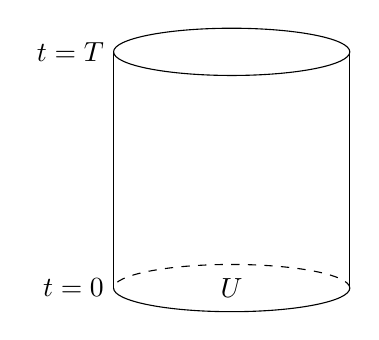
\begin{tikzpicture}
    \draw (1.5, 0) arc (0:-180:1.5 and 0.3);
    \draw [dashed] (1.5, 0) arc (0:180:1.5 and 0.3);
    \draw (1.5, 0) -- (1.5, 3);
    \draw (-1.5, 0) -- (-1.5, 3);

    \draw (0, 3) ellipse (1.5 and 0.3);

    \node [left] at (-1.5, 0) {$t = 0$};
    \node [left] at (-1.5, 3) {$t = T$};

    \node at (0, 0) {$U$};
  \end{tikzpicture}
\end{center}
We define
\begin{align*}
  U_t &= (0, t) \times U\\
  \Sigma_t &= \{t\} \times U\\
  \partial^* U_t &= [0, t] \times \partial U.
\end{align*}
Then
\[
  \partial U_T = \Sigma_0 \sqcup \Sigma_T \sqcup \partial^* U_T.
\]
The general \term{initial boundary value problem} (IVBP)\index{IBVP} is as follows: Let $L$ be a (time-dependent) uniformly elliptic operator. We want to solve
\begin{align*}
  u_{tt} + L u &= f && \text{on }U_T\\
  u &= \psi &&\text{on }\Sigma_0\\
  u_t &= \psi' && \text{on }\Sigma_0\\
  u &= 0 && \text{on } \partial^* U_T.
\end{align*}
In the case of elliptic PDEs, we saw that Laplace's equation was a canonical, motivating example. In this case, if we take $L = - \Delta$, then we obtain the \term{wave equation}. Let's see what we can do with it.

\begin{eg}
  Start with the equation $u_{tt} - \Delta u = 0$. Multiply by $u_t$ and integrate over $U_t$ to obtain
  \begin{align*}
    0 &= \int_{U_t} \Big(u_{tt} u_t - u_t \Delta u\Big) \;\d x\;\d t\\
    &= \int_{U_t} \left[\frac{1}{2}\frac{\partial}{\partial t} u_t^2 - \nabla \cdot (u_t \D u) + \D u_t \cdot \D u\right]\;\d x\;\d t\\
    &= \int_{U_t} \left[\frac{1}{2}\frac{\partial}{\partial t} \left( u_t^2 + |\D u|^2\right) - \nabla \cdot (u_t D u)\right]\;\d x\;\d t\\
    &= \frac{1}{2} \int_{\Sigma_t - \Sigma_0} \Big(u_t^2 + |\D u|^2\Big)\;\d x - \int_{\partial^* U_t} u_t \frac{\partial u}{\partial \nu}\;\d S.
  \end{align*}
  But $u$ vanishing on $\partial^* U_T$ implies $u_t$ vanishes as well. So the second term vanishes, and we obtain
  \[
    \int_{\Sigma_t} u_t^2 + |\D u|^2 \;\d x = \int_{\Sigma_0} u_t^2 + |\D u|^2 \;\d x.
  \]
  This is the conservation of energy! Thus, if a solution exists, we control $\|u\|_{H^1(\Sigma_t)}$ in terms of $\|\psi\|_{H^1(\Sigma_0)}$ and $\|\psi'\|_{L^2(\Sigma_0)}$. We also see that the solution is uniquely determined by $\psi$ and $\psi'$, since if $\psi = \psi' = 0$, then $u_t = \D u = 0$ and $u$ is zero at the boundary.
\end{eg}

Estimates like this that control a solution without needing to construct it are known as \term{a priori estimates}. These are often crucial to establish the existence of solutions (cf.\ G\r{a}rding).

%Returning to the general case, let us define
%\[
%  Lu = -\sum_{i, j = 1}^n (a^{ij}(x, t) u_{x_j})_{x_i} + \sum_{i = 1}^n b^i(x, t) u_{x_i} + c(x, t) u,
%\]
%for $a^{ij} = a^{ji}, b^i, c \in C^1(\bar{U}_T)$. We further assume the uniform ellipticity condition, i.e.\ there exists $\theta > 0$ such that
%\[
%  \sum_{i, j = 1}^n a^{ij}(x, t) \xi_i \xi_j \geq \theta |\xi|^2.
%\]
%The initial boundary value problem we are going to consider is
%\begin{align*}
%  u_{tt} + Lu &= f&\text{on }U_T\\
%  u &= \psi &\text{on }\Sigma_0\\
%  u_t &= \psi' & \text{on }\Sigma_0\\
%  u &= 0 &\text{on } \partial^* U_T
%\end{align*}

We shall first find a weak formulation of this problem that only requires $u \in H^1(U_T)$. Note that when we do so, we have to understand carefully what we mean by $u_t = \psi'$. We shall see how we will deal with that in the derivation of the weak formulation.

Assume that $u \in C^2(\bar{U}_T)$ is a classical solution. Multiply the equation by $v \in C^2(\bar{U}_T)$ which satisfies $v = 0$ on $\partial^* U_T \cup \Sigma_T$. Then we have
\begin{align*}
  \int_{U_T} \d x\;\d t\; (fv) &= \int_{U_T} \d x\;\d t\; (u_{tt}v + Luv)\\
  &= \int_{U_T} \d x\;\d t\left(-u_t v_t + \sum a^{ij} u_{x_i} v_{x_j} + \sum b^i u_{x_i v} + cu\right)\\
  &\phantomeq + \left[\int_U u_t v \;\d x\right]_0^T - \int_0^T \;\d t \left(\int_{\partial U} \sum a^{ij} u_{x_j} v\;\d S\right)\;\d t.
\end{align*}
Using the boundary conditions, we find that
\begin{multline*}
  \int_{U_T} fv\;\d x \;\d t = \int_{U_T} \left(-u_t v_t + \sum a^{ij} u_{x_i} v_{x_j} + \sum b^i u_{x_i} v + cuv \right)\;\d x\;\d t \\
  - \int_{\Sigma_0} \psi' v\;\d x.\tag{$\dagger$}
\end{multline*}
Conversely, suppose $u \in C^2(\bar{U}_T)$ satisfies $(\dagger)$ for all such $v$, and $u|_{\Sigma_0} = \psi$ and $u|_{\partial^* U_T} = 0$. Then by first testing on $v \in C_c^\infty(U_T)$, reversing the integration by parts tells us
\[
  0 = \int_{U_T} (u_{tt} + Lu - f)v\;\d x,
\]
since there is no boundary term. Hence we get
\[
  u_{tt} + Lu = f
\]
on $U_T$. To check the boundary conditions, if $v \in C^\infty(\bar{U}_T)$ vanishes on $\partial^*U_T \cup \Sigma_T$, then again reversing the integration by parts shows that
\[
  \int_{U_T} (u_{tt} + Lu - f) v\;\d x \;\d t = \int_{\Sigma_0} (\psi' - u_t) v\;\d x.
\]
Since we know that the LHS vanishes, it follows that $\psi' = u_t$ on $\Sigma_0$. So we see that our weak formulation can encapsulate the boundary condition on $\Sigma_0$.

\begin{defi}[Weak solution]\index{weak solution!hyperbolic equation}
  Suppose $f \in L^2(U_T)$, $\psi \in H_0^1(\Sigma_0)$ and $\psi' \in L^2(\Sigma_0)$. We say $u \in H^1(U_t)$ is a weak solution to the hyperbolic PDE if
  \begin{enumerate}
    \item $u|_{\Sigma_0} = \psi$ in the trace sense;
    \item $u|_{\partial^* U_T} = 0$ in the trace sense; and
    \item $(\dagger)$ holds for all $v \in H^1(U_T)$ with $v = 0$ on $\partial^* U_T \cup \Sigma_T$ in a trace sense.
  \end{enumerate}
\end{defi}

\begin{thm}[Uniqueness of weak solution]\index{uniqueness theorem!hyperbolic equation}
  A weak solution, if exists, is unique.
\end{thm}
%The non-trivial part of this theorem is that we cannot use $u_t$ as the test function.

\begin{proof}
  It suffices to consider the case $f = \psi = \psi' = 0$, and show any solution must be zero. Let
  \[
    v(x, t) = \int_t^T e^{-\lambda s} u(x, s)\;\d s,
  \]
  where $\lambda$ is a real number we will pick later. The point of introducing this $e^{-\lambda t}$ is that in general, we do not expect conservation of energy. There could be some exponential growth in the energy, so want to suppress this.

  Then this function belongs to $H^1(U_T)$, $v = 0$ on $\Sigma_T \cup \partial^* U_T$, and
  \[
    v_t = -e^{-\lambda t} u.
  \]
  Using the fact that $u$ is a weak solution, we have
  \[
    \int_{U_T} \left( u_t u e^{- \lambda t} - \sum v_{t x_j} v_{x_i} e^{\lambda t} + \sum_i b^i u_{x_i} v + (c - 1) uv - v v_t e^{\lambda t}\right)\;\d x \;\d t = 0.
  \]
  Integrating by parts, we can write this as $A = B$, where
  \begin{align*}
    A &= \int_{U_T} \left( \frac{\d}{\d t} \left(\frac{1}{2} u^2 e^{-\lambda t} - \sum a^{ij} v_{x_i} v_{x_j} e^{\lambda t} - \frac{1}{2} v^2 e^{\lambda t}\right) \right.\\
    &\phantomeq \hphantom{\int_{U_T}} \left.+ \frac{\lambda}{2} \left(u^2 e^{-\lambda t} + \sum a^{ij} v_{x_i} v_{x_j} e^{\lambda t} + v^2 e^{\lambda t}\right)\right) \;\d x\;\d t\\
    B &= - \int_{U_T} \left(e^{\lambda t} \sum a^{ij} v_{x_i} v_{x_j} - \sum b^i_{x_i} uv - \sum b^i v_{x_i} u + (c - 1) uv\right) \;\d x\;\d t.
  \end{align*}
  Here $A$ is the nice bit, which we can control, and $B$ is the junk bit, which we will show that we can absorb elsewhere.

  Integrating the time derivative in $A$, using $v = 0$ on $\Sigma_T$ and $u = 0$ on $\Sigma_0$, we have
  \begin{multline*}
    A = e^{\lambda T} \int_{\Sigma_T} \frac{1}{2} u^2 \;\d x + \int_{\Sigma_0} \sum \left(a^{ij} v_{x_i} v_{x_j} + v^2\right) \;\d x\\
    \frac{\lambda}{2} \int_{U_T}\left(u^2 e^{-\lambda t} + \sum a^{ij} v_{x_i} v_{x_j} e^{\lambda t} + v^2 e^{\lambda t}\right) \;\d x\;\d t.
  \end{multline*}
  Using the uniform ellipticity condition (and the observation that the first line is always non-negative), we can bound
  \[
    A \geq \frac{\lambda}{2} \int_{U_T} \left(u^2 e^{-\lambda t} + \theta |\D v|^2 e^{\lambda t} + v^2 e^{\lambda t}\right)\;\d x\;\d t.
  \]
  Doing some integration by parts, we can also bound
  \[
    B \leq \frac{c}{2} \int_{U_T} \left(u^2 e^{-\lambda t} + \theta |\D v|^2 e^{\lambda t} + v^2 e^{\lambda t}\right)\;\d x\;\d t,
  \]
  where the constant $c$ does not depend on $\lambda$. Taking this together, we have
  \[
    \frac{\lambda - c}{2} \int_{U_T} \left(u^2 e^{-\lambda t} + \theta |\D v|^2 e^{\lambda t} + v^2 e^{\lambda t}\right)\;\d x\;\d t \leq 0.
  \]
  Taking $\lambda > c$, this tells us the integral must vanish. In particular, the integral of $u^2 e^{\lambda t} = 0$. So $u = 0$.
\end{proof}
%For those who know GR/the vector field method, this is using
%\[
%  X = e^{-\lambda t} \partial_t
%\]
%as a multiplier.

We now want to prove the existence of weak solutions. While we didn't need to assume much regularity in the uniqueness result, since we are going to subtract the boundary conditions off anyway, we expect that we need more regularity to prove existence.
\begin{thm}[Existence of weak solution]\index{existence theorem!hyperbolic equation}
  Given $\psi \in H_0^1(U)$ and $\psi' \in L^2(U)$, $f \in L^2(U_T)$, there exists a (unique) weak solution with
  \[
    \|u\|_{H^1(U_T)} \leq C (\|\psi\|_{H^1(U)} + \|\psi'\|_{L^2(U)} + \|f\|_{L^2(U_T)}).\tag{$\dagger$}
  \]
\end{thm}
\begin{proof}
  We use \term{Galerkin's method}. The way we write our equations suggests we should think of our hyperbolic PDE as a second-order ODE taking values in the infinite-dimensional space $H^1_0(U)$. To apply the ODE theorems we know, we project our equation onto a finite-dimensional subspace, and then take the limit.

  First note that by density arguments, we may assume $\psi, \psi' \in C_c^\infty(U)$ and $f \in C_c^\infty(U_T)$, as long as we prove the estimate ($\dagger$). So let us do so.

  Let $\{\varphi_k\}_{k = 1}^\infty$ be an orthonormal basis for $L^2(U)$, with $\varphi_k \in H_0^1(U)$. For example, we can take $\varphi_k$ to be eigenfunctions of $-\Delta$ with Dirichlet boundary conditions.

  We shall consider ``solutions'' of the form
  \[
    u^N(x, t) = \sum_{k = 1}^N u_k(t) \varphi_k(x).
  \]
  We want this to be a solution after projecting to the subspace spanned by $\varphi_1, \ldots, \varphi_N$. Thus, we want $(u_{tt} + Lu - f, \varphi_k)_{L^2(\Sigma_t)} = 0$ for all $k = 1,\ldots, N$. After some integration by parts, we see that we want
  \[
    \left(\ddot{u}^N, \varphi_k\right)_{L^2(U)} + \int_{\Sigma_t} \left(\sum a^{ij} u_{x_i}^N (\varphi_k)_{x_j} + b^i u_{x_i}^N \varphi_k + c u^N \varphi_k\right) \;\d x = (f, \varphi_k)_{L^2(U)}.\tag{$*$}
  \]
  We also require
  \begin{align*}
    u_k(0) &= (\psi, \varphi_k)_{L^2(U)}\\
    \dot{u}_k(0) &= (\psi', \varphi_k)_{L^2(U)}.
  \end{align*}
  Notice that if we have a genuine solution $u$ that can be written as a finite sum of the $\varphi_k(x)$, then these must be satisfied.

  This is a system of ODEs for the functions $u_k(t)$, and the RHS is uniformly $C^1$ in $t$ and linear in the $u_k$'s. By Picard--Lindel\"of, a solution exists for $t \in [0, T]$.

  So for each $N$, we have an approximate solution that solves the equation when projected onto $\bra \varphi_1, \ldots, \varphi_N\ket$. What we need to do is to extract from this solution a genuine weak solution. To do so, we need some estimates to show that the functions $u^N$ converge.

  We multiply $(*)$ by $e^{-\lambda t} \dot{u}_k(t)$, sum over $k = 1, \ldots, N$, and integrate from $0$ to $\tau \in (0, T)$, and end up with
  \begin{multline*}
    \int_0^\tau \;\d t \int_U \;\d x \left(\ddot{u}^N \dot{u}^N e^{-\lambda t} + \sum a^{ij} u_{x_i}^N \dot{u}_{x_j}^N + \sum b^i u_{x_i}^N \dot{u}^N + c u^N \dot{u}^N\right)e^{-\lambda t}\\
    = \int_0^\tau \;\d t \int_U \;\d u (f \dot{u}_N e^{-\lambda t}).
  \end{multline*}
  As before, we can rearrange this to get $A = B$, where
  \begin{multline*}
    A = \int_{U_\tau}\d t \;\d x \left(\frac{\d}{\d t} \left(\frac{1}{2} (\dot{u}^N)^2 + \frac{1}{2} \sum a^{ij} u_{x_i}^N u_{x_j}^N + \frac{1}{2} (u^N)^2 e^{-\lambda t}\right)\right.\\
    \left.+ \frac{\lambda}{2} \left((\dot{u}^N)^2 + \sum a^{ij} u_{x_i}^N u_{x_j}^N + (u^N)^2 \right)e^{-\lambda t}\right)
  \end{multline*}
  and
  \[
    B = \int_{U_\tau} \d t\;\d x\left( \frac{1}{2} \sum \dot{a}^{ij} u_{x_i}^N u_{x_j}^N - \sum b^i u_{x_i}^N \dot{u}^N + (1 - c) u^N \dot{u}^N + f \dot{u}^N \right)e^{-\lambda t}.
  \]
  Integrating in time, and estimating as before, for $\lambda$ sufficiently large, we get
  \begin{multline*}
    \frac{1}{2} \int_{\Sigma_\tau} \Big((\dot{u}^N)^2 + |\D u^N|^2\Big) \;\d x + \int_{U_\tau} \Big((\dot{u}^N)^2 + |\D u^N|^2 + (u^N)^2\Big) \;\d x\;\d t\\
    \leq C (\|\psi\|^2_{H^1(U)} + \|\psi'\|^2_{L^2(U)} + \|f\|_{U_T}^2).
  \end{multline*}
  This, in particular, tells us $u^N$ is bounded in $H^1(U_T)$,

  Since $u^N(0) = \sum_{n = 1}^N (\psi, \varphi_k) \varphi_k$, we know this tends to $\psi$ in $H^1(U)$. So for $N$ large enough, we have
  \[
    \|u^N\|_{H^1(\Sigma_0)} \leq 2 \|\psi\|_{H^1(U)}.
  \]
  Similarly, $\|\dot{u}^N\|_{L^2(\Sigma_0)} \leq 2 \|\psi'\|_{L^2(U)}$.

  Thus, we can extract a convergent subsequence $u^{N_m} \rightharpoonup u$ in $H^1(U)$ for some $u \in H^1(U)$ such that % u \in H_0^1(U) ?
  \[
    \|u\|_{H^1(U_T)} \leq C (\|\psi\|_{H^1(U)} + \|\psi\|_{L^2(U)} + \|f\|_{L^2(U_T)}).
  \]
  For convenience, we may relabel the sequence so that in fact $u^N \rightharpoonup u$.

  To check that $u$ is a solution, suppose $v = \sum_{k = 1}^M v_k(t) \varphi_k$ for some $v_k \in H^1((0, T))$ with $v_k(T) = 0$. By definition of $u^N$, we have
  \[
    (\ddot{u}^N, v)_{L^2(U)} + \int_{\Sigma_t} \sum_{i, j} a^{ij} u_{x_i}^N v_{x_j} + \sum_i b^i u_{x_i}^N v + cuv \;\d x = (f, v)_{L^2(U)}.
  \]
  Integrating $\int_0^T \;\d t$ using $v(T) = 0$, we have
  \begin{multline*}
    \int_{U_T} \left(-u_t^N v_t + \sum{x_i}^N v_{x_j} + \sum b^i u_{x_i}^N v + cuv\right) \;\d x \;\d t - \int_{\Sigma_0} u_t^N v\;\d x \\
    = \int_{U_T} fv\;\d x\;\d t.
  \end{multline*}
  Now note that if $N > M$, then $\int_{\Sigma_0} u_t^N v\;\d x = \int_{\Sigma_0} \psi' v \;\d x$. Now, passing to the weak limit, we have
  \begin{multline*}
    \int_{U_T} \left(-u_t v_t + \sum a^{ij} u_{x_i} v_{x_j} + \sum b^i u_{x_i} v + cuv\right) \;\d x \;\d t - \int_{\Sigma_0}\psi' v\;\d x \\
    = \int_{U_T} fv\;\d x\;\d t.
  \end{multline*}
  So $u_t$ satisfies the identity required for $u$ to be a weak solution.

  Now for $k = 1, \ldots, M$, the map $w \in H^1(U_T) \mapsto \int_{\Sigma_0} w \varphi_k \;\d x$ is a bounded linear map, since the trace is bounded in $L^2$. So we conclude that
  \[
    \int_{\Sigma_0} u \varphi_k \;\d x = \lim_{N \to \infty} \int_{\Sigma_0} u^N \varphi_k \;\d x = (\psi, \varphi_k)_{L^2(H)}.
  \]
  Since this is true for all $\varphi_k$, it follows that $u|_{\Sigma_0} = \psi$, and $v$ of the form considered are dense in $H^1(U_T)$ with $v = 0$ on $\partial^*U_T \cup \Sigma_T$. So we are done.
\end{proof}

In fact, we have
\[
  \esssup_{t \in (0, T)} (\|\dot{u}\|_{L^2(\Sigma_t)} + \|u\|_{H^1(\Sigma_t)}) \leq C \cdot (\mathrm{data}).
\]
So we can say $u \in L^\infty( (0, T), H^1(U))$ and $\dot{u} \in L^\infty((0, T), L^2(U))$.

%Note that although the energy $\|\dot{u}\|_{L^2(\Sigma_t)} + \|u\|_{H^2(\Sigma_t)}$ is bounded, we cannot conclude that the energy is continuous.

We would like to improve the regularity of the solution. To motivate how we are going to do that, let's go back to the wave equation for a bit.

Suppose that in fact $u \in C^\infty(U_T)$ is a smooth solution to the wave equation with initial conditions $(\psi, \psi')$. We want a quantitative estimate for $u \in H^2(\Sigma_t)$. The idea is to differentiate the equation with respect to $t$. Writing $w = u_t$, we get
\begin{align*}
  w_{tt} - \Delta w &= 0\\
  w|_{\Sigma_0} &= \psi'\\
  w_t|_{\Sigma_0} &= \Delta \psi\\
  w|_{\partial^* U_T} &= 0.
\end{align*}
By the energy estimate we have for the wave equation, we get
\begin{align*}
  \|w_t\|_{L^2(\Sigma_t)} + \|w\|_{H^1(\Sigma_t)} &\leq C(\|\psi'\|_{H^1(U)} + \|\Delta \psi\|_{L^2(U)})\\
  &\leq C(\|\psi'\|_{H^1(U)} + \|\psi\|_{H^2(U)}).
\end{align*}
So we now have control of $u_{tt}$ and $u_{tx_i}$ in $L^2(\Sigma_t)$. But once we know that $u_{tt}$ is controlled in $L^2$, then we can use the elliptic estimate to gain control on the second-order spatial derivatives of $u$. So
\[
  \|u\|_{H^2(\Sigma_t)}\leq C(\|\Delta u\|_{L^2(\Sigma_t)}) = C \|u_{tt}\|_{L^2(\Sigma_t)}.
\]
So we control all second-derivatives of $u$ in terms of the data.

\begin{thm}
  If $a^{ij}, b^i, c \in C^2(U_T)$ and $\partial U \in C^2$, then for $\psi \in H^2(U)$ and $\psi' \in H_0^1(U)$, and $f, f_t \in L^2(U_T)$, we have
  \begin{align*}
    u &\in H^2(U_T) \cap L^\infty((0, T); H^2(U))\\
    u_t &\in L^\infty((0, T), H_0^1(U))\\
    u_{tt} &\in L^\infty((0, T); L^2(U))
  \end{align*}
\end{thm}

\begin{proof}
  We return to the Galerkin approximation. Now by assumption, we have a linear system with $C^2$ coefficients. So $u_k \in C^3((0, T))$. Differentiating with respect to $t$ (assuming as we can $f, f_t \in C^0(\bar{U}_T)$), we have
  \begin{multline*}
    (\partial_t^3 u^N, \varphi_k)_{L^2(U)} + \int_{\Sigma_t} \left(\sum a^{ij} \dot{u}_{x_i}^N (\varphi_k)_{x_j} + \sum b^i \dot{u}_{x_i}^N \varphi_k + c \dot{u}^N \varphi_k \right) \;\d x\\
    = (\dot{f}, \varphi_k)_{L^2(U)} - \int_{\Sigma_t} \left( \sum \dot{a}^{ij} u_{x_i}^N (\varphi_k)_{x_j} + \sum \dot{b}^i u_{x_i}^N \varphi_k + \dot{c} u \varphi_k \right)\;\d x.
  \end{multline*}
  Multiplying by $\ddot{u}_k e^{-\lambda t}$, summing $k = 1, \ldots, N$, integrating $\int_0^\tau \;\d t$, and recalling we already control $u \in H^1(U_T)$, we get
  \begin{multline*}
    \sup_{t \in (0, T)} (\|u_t^N\|_{H^1(\Sigma_t)} + \|u_{tt}^N\|_{L^2(\Sigma_t)} + \|u_t^N\|_{H^2(U_T)})\\
    \leq C\Big(\|u_t^N\|_{H^1(\Sigma_0)} + \|u_{tt}^N\|_{L^2(\Sigma_0)} + \|\psi\|_{H^1(\Sigma_0)} \\
    + \|\psi'\|_{L^2(\Sigma_0)} + \|f\|_{L^2(U_T)} + \|f_t\|_{L^2(U_T)}\Big).
  \end{multline*}
  We know
  \[
    u_t^N|_{t = 0} = \sum_{k = 1}^N (\psi', \varphi_k)_{L^2(U)} \varphi_k.
  \]
  Since $\varphi_k$ are a basis for $H^1$, we have
  \[
    \|u_t^N\|_{H^1(\Sigma_0)} \leq \|\psi'\|_{H^1(\Sigma_0)}.
  \]
  To control $u^N_{tt}$, let us assume for convenience that in fact $\varphi_k$ are the eigenfunctions $-\Delta$. From the fact that
  \[
    (\ddot{u}^N, \varphi_k)_{L^2(U)} + \int_{\Sigma_t} \sum_{i, j} a^{ij} u_{x_i}^N (\varphi_k)_{x_j} + \sum_i b^i u_{x_i}^N \varphi_k + c u^N \varphi_k\;\d x\;\d t = (f, \varphi_k)_{L^2(U)},
  \]
  integrate the first term in the integral by parts, multiply by $\ddot{u}_n$, and sum to get
  \[
    \|u_{tt}^N\|_{\Sigma_0} \leq C(\|u^N\|_{H^2(\Sigma_0)} + \|f\|_{L^2(U_T)} + \|f_t\|_{L^2(U_T)}).
  \]
  We need to control $\|u^N\|_{H^2(\Sigma_0)}$ by $\|\psi\|_{H^2(\Sigma_0)}$. Then, using that $\Delta\varphi_k|_{\partial U} = 0$ and $u^N$ is a finite sum of these $\varphi_k$'s,
  \[
    (\Delta u^N, \Delta u^N)_{L^2\!(\Sigma_0)} = (u^N, \Delta^2 u^N)_{L^2\!(\Sigma_0)} = (\psi, \Delta^2 u^N)_{L^2\!(\Sigma_0)} = (\Delta \psi, \Delta u^N)_{L^2\!(\Sigma_0)}.
  \]
  So
  \[
    \|u^N\|_{H^2(\Sigma_0)} \leq \|\Delta u^N\|_{L^2(\Sigma_0)} \leq C \|\psi\|_H^2(U).
  \]
  Passing to the weak limit, we conclude that
  \begin{align*}
    u_t &\in H^1(U_T)\\
    u_t &\in L^\infty((0, T), H_0^1(U))\\
    u_{tt} &\in L^\infty((0, T), L^2(U)).
  \end{align*}
  Since $u_{tt} + Lu = f$, by an elliptic estimate on (almost) every constant $t$, we obtain $u \in L^\infty((0, T), H^2(U))$.
\end{proof}

We can now understand the equation as holding pointwise almost everywhere by undoing the integration by parts that gave us the definition of the weak solution. The initial conditions can also be understood in a trace sense.

Returning to the case $\psi \in H^1_0(U)$ and $\psi' \in L^2(U)$, by approximating in $H^2(U)$, by approximating in $H^2(U)$, $H_0^1(U)$ respectively, we can show that a weak solution can be constructed as a \emph{strong} limit in $H^1(U_T)$. This implies the energy identity, so that in fact weak solutions satisfy
\begin{align*}
  u &\in C^0((0, T); H_0^1(U))\\
  u_t &\in C^0((0, T); L^2(U))
\end{align*}
This requires slightly stronger regularity assumptions on $a^{ij}$, $b^i$ and $c$. Such solutions are said to be in the \term{energy class}.

Finally, note that we can iterate the argument to get higher regularity.
\begin{thm}
  If $a^{ij}, b^i, c \in C^{k + 1}(\bar{U}_T)$ and $\partial U$ is $C^{k + 1}$, and
  \begin{align*}
    \partial^i_t u|_{\Sigma_0} &\in H_0^1 (U)&i &= 0, \ldots, k\\
    \partial_t^{k + 1}u |_{\Sigma_0} &\in L^2(U)\\
    \partial_t^i f &\in L^2((0, T); H^{k - i}(U)) & i &= 0, \ldots, k
  \end{align*}
  then $u \in H^{k + 1}(U)$ and
  \[
    \partial_t^i u \in L^\infty((0, T); H^{k + 1 - i}(U))
  \]
  for $i = 0, \ldots, k + 1$.

  In particular, if everything is smooth, then we get a smooth solution.
\end{thm}
The first two conditions should be understood as conditions on $\psi$ and $\psi'$, using the fact that the equation allows us to express higher time derivatives of $u$ in terms of lower time derivatives and spatial derivatives. One can check that these condition imply $\psi \in H^{k + 1}(U)$ and $\psi' \in H^k(U)$, but the condition we wrote down also encodes some compatibility conditions, since we know $u$ ought to vanish at the boundary, hence all time derivatives should.

%For example, consider the wave equation
%\[
%  u_{tt} - \Delta u = 0.
%\]
%with $u = \psi, u_t = \psi'$ at $\Sigma_0$ and $u = 0$ on $\partial^* U_t$. If we have a smooth solution, then $u_{tt} = 0$ on $\partial^* U_T$. So $\Delta u = 0$ on $\partial^* U_T$. So $\Delta \psi$ on $\partial^* U_T$.

Those were the standard existence and regularity theorems for hyperbolic PDEs. However, there are more things to say about hyperbolic equations. The ``physicist's version'' of the wave equation involves a constant $c$, and says
\[
  \ddot{u} - c^2 \Delta x = 0.
\]
This constant $c$ is the speed of propagation. This tells us in the wave equation, information propagates at a speed of at most $c$. We can see this very concretely in the $1$-dimensional wave equation, where d'Alembert wrote down an explicit solution to the wave equation given by
\[
  u(x, t) = \frac{1}{2} (\psi(x - ct) + \psi(x + ct)) + \frac{1}{2c} \int_{x - ct}^{x + ct} \psi'(y) \;\d y.
\]
Thus, we see that the value of $\phi$ at any point $(x, t)$ is \emph{completely} determined by the values of $\psi$ and $\psi'$ in the interval $[x - ct, x + ct]$.
\begin{center}
  \begin{tikzpicture}
    \node at (-1.5, 2) [circ] {};
    \node at (-1.5, 2) [above] {$(x, t)$};
    \fill [mgreen, opacity=0.5] (-3.5, 0) -- (-1.5, 2) -- (0.5, 0) -- cycle;
    \draw (-3.5, 0) -- (-1.5, 2) -- (0.5, 0);

    \draw [mred] (-4, 0) -- (1, 0) node [right] {$t = 0$};
  \end{tikzpicture}
\end{center}

This is true for a general hyperbolic PDE. In this case, the speed of propagation should be measured by the principal symbol $Q(\xi) = \sum a^{ij}(y) \xi_i \xi_j$. The correct way to formulate this result is as follows:

Let $S_0 \subseteq U$ be an open set with (say) smooth boundary. Let $\tau: S_0 \to [0, T]$ be a smooth function vanishing on $\partial S_0$, and define
\begin{align*}
  D &= \{(t, x) \in U_T : x \in S_0, 0 < t < \tau(x)\}\\
  S' &= \{(\tau(x), x): x \in S_0\}.
\end{align*}
We say $S'$ is \term{spacelike} if
\[
  \sum_{i, j = 1}^n a^{ij} \tau_{x_i} \tau_{x_j} < 1
\]
for all $x \in S_0$.

\begin{thm}
  If $u$ is a weak solution of the usual thing, and $S'$ is spacelike, then $u|_D$ depends only on $\psi|_{S_0}, \psi'|_{S_0}$ and $f|_{D}$.
\end{thm}
The proof is rather similar to the proof of uniqueness of solutions.

\begin{proof}
  Returning to the definition of a weak solution, we have
  \[
    \int_{U_T} - u_t v_t + \sum_{i, j = 1}^{n} a^{ij} u_{x_j} v_{x_i} + \sum_{i = 1}^n b^i u_{x_i} + cuv \;\d x \;\d t - \int_{\Sigma_0} \psi' v \;\d x = \int_{U_T} fv \;\d x\;\d t.
  \]
  By linearity it suffices to show that if $u|_{\Sigma_0} = 0$ if $\psi|_{S_0} = \psi' |_{S_0} = 0$ and $f|_D = 0$. We take as test function
  \[
    v(t, x) =
    \begin{cases}
      \int_t^{\tau(x)} e^{-\lambda s} u(s, x)\;\d s & (t, x) \in D\\
      0 & (t, x) \not \in D
    \end{cases}.
  \]
  One checks that this is in $H^1(U_T)$, and $v = 0$ on $\Sigma_T \cup \partial^* U_T$ with
  \begin{align*}
    v_{x_i} &= \tau_{x_i} e^{-\lambda \tau} u(x, \tau) + \int_t^{\tau(x)} e^{-\lambda s} u_{x_i} (x, s) \;\d s\\
    v_t &= -e^{-\lambda t} u(x, t).
  \end{align*}
  Plugging these into the definition of a weak solution, we argue as in the previous uniqueness proof. Then
  \begin{multline*}
    \int_D \frac{\d}{\d t} \left(\frac{1}{2} u^2 e^{-\lambda t} - \frac{1}{2} \sum a^{ij} v_{x_i} v_{x_j} e^{\lambda t} - \frac{1}{2} v^2 e^{\lambda t}\right)\\
    + \frac{\lambda}{2} \left(u^2 e^{-\lambda t} + \sum a^{ij} v_{x_i} v_{x_j} e^{\lambda t}+ v^2 e^{\lambda t}\right)\;\d x\;\d t\\
    = \int_D \left(\frac{1}{2} \sum a^{ij} v_{x_i} v_{x_j} e^{\lambda t} - \sum b^i v_{x_i} v - (c - 1) uv\right)\;\d x\;\d t
  \end{multline*}
  Noting that $\int_D \;\d x \;\d t = \int_{S_0} \;\d x \int_0^{\tau(x)}\;\d t$, we can perform the $t$ integral of the $\frac{\d}{\d t}$ term, and we get contribution from $S'$ which is given by
  \[
    I_{S'} =\int_{S_0}\left(\frac{1}{2} u^2 (\tau(x), x) e^{-\lambda \tau(x)} - \frac{1}{2} \sum_{i, j} a^{ij} \tau_{x_i} \tau_{x_j} u^2 e^{-\lambda \tau}\right)\;\d x
  \]
  We have used $v = 0$ on $S'$ and $v_{x_i} = \tau_{x_i} u e^{-\lambda \tau}$. Using the definition of a spacelike surface, we have $I_{S'} > 0$. The rest of the argument of the uniqueness of solutions goes through to conclude that $u = 0$ on $D$.
\end{proof}
This implies no signal can travel faster than a certain speed. In particular, if
\[
  \sum_{i, j} a^{ij} \xi_i \xi_j \leq \mu |\xi|^k
\]
for some $\mu$, then no signal can travel faster than $\sqrt{\mu}$. This allows us to solve hyperbolic equations on unbounded domains by restricting to bounded domains.
\printindex
\end{document}
